% -*- root: ../Thesis.tex -*-
\chapter{Wyniki i ich analiza}
\label{chap:wyniki}


\section{Istnienie rozwiązań}

Podstawowym pytaniem matematycznym, na jakie należy odpowiedzieć przy rozpatrywaniu układu (\ref{eq:1})-(\ref{eq:5}) jest pytanie o istnienie rozwiązań. Ponieważ zainteresowani jesteśmy rozwiązaniami periodycznymi w czasie, istnienie rozwiązań musi mieć charakter globalny w czasie. Ze względu na interpretację biologiczną musimy również pokazać, że składowe rozwiązania są funkcjami nieujemnymi. Zagadnienie nieujemności rozwiązań może być rozważone w oparciu o następujące twierdzenie. 

\medskip 

\begin{thm} \label{th:chepyzov} 

(Propozycja 1.1 z \cite{Chepyzhov2002}) Podzbiór $\mathbb{R}^N$ (zbiór punktów o nieujemnych składowych przestrzeni $\mathbb{R}^N$) jest niezmienniczy względem przepływu opisanego równaniem

\[
\frac{du}{dt} = F(u), 
\]
 wtedy i tylko wtedy, gdy dla każdego  \mbox{$i=1,\ldots,N$} funkcja 
$F(u):\mathbb{R}^N_+ \to \mathbb{R}^N_+$, $N \ge 1$, $u:=(u_1,\ldots,u_N)$, spełnia warunek:  
\begin{equation} \label{warch} 
F_i(u_1,\ldots,0,\ldots,u_N) \geq 0,
\end{equation} 
\noindent gdzie $0$ przypisane jest składowej $u_i$ a $u_j \geq 0$ dla $j \neq i$.
\end{thm}

\noindent Używając powyższego twierdzenia oraz prawa zachowania danego równaniem (\ref{eq:cons:Ca}) udowodnimy istnienie nieujemnych rozwiązań dla układów niezredukowanych (\ref{eq:1})--(\ref{eq:5}) i (\ref{eq:1aa})--(\ref{eq:5aa}), a co za tym idzie układów zredukowanych (\ref{eq:1a})--(\ref{eq:3a}) oraz (\ref{eq:11})--(\ref{eq:33}). 

\begin{thm} \label{ist1}
Załóżmy, że warunki początkowe $Ca_{Cyt}(0)$, $Ca_{ER}(0)$, $Ca_{Mit}(0)$, $CaPr(0)$ oraz $Pr(0)$ są nieujemne. Wtedy rozwiązania równań (\ref{eq:1})--(\ref{eq:5}) istnieją globalnie w~czasie, są jednoznacznie określone i nieujemne. 
\end{thm}

\begin{proof}
Wykażemy najpierw, że prawe strony układu (\ref{eq:1})--(\ref{eq:5}) spełniają warunki (\ref{warch}). Mamy zatem: 

\begin{eqnarray*}
F_1(0,Ca_{ER},Ca_{Mit}, CaPr, Pr)  &=& k_{leak} Ca_{ER} + k_m Ca_{Mit} 
							+ K_- CaPr, \\
F_2(Ca_{Cyt},0,Ca_{Mit}, CaPr, Pr) &=& 
							\frac{\beta_{ER}}{\rho_{ER}}\Bigg(k_{pump}Ca_{Cyt} 
							+ k_{ch} \frac{Ca_{Cyt}^3}{K_1^2+Ca_{Cyt}^2} 
							+ k_{leak}Ca_{Cyt} \Bigg), \\
F_3(Ca_{Cyt},Ca_{ER},0, CaPr, Pr)	 &=& \frac{\beta_{Mit}}{\rho_{Mit}} 
							\left(k_{in}\frac{Ca_{Cyt}^8}{K_2^8+Ca_{Cyt}^8} 
							+k_{MAM}\frac{Ca_{ER}^8}{K_4^8+Ca_{ER}^8} \right), \\
F_4(Ca_{Cyt},Ca_{ER},Ca_{Mit}, 0, Pr) &=& k_+ Ca_{Cyt}Pr, \\
F_5(Ca_{Cyt},Ca_{ER},Ca_{Mit}, CaPr, 0) &=& k_- CaPr.							
\end{eqnarray*}

\noindent Prawe strony powyższych równości są nieujemne dla $Ca_{Cyt}$, $Ca_{Mit}$, $Ca_{ER}$, $CaPr$ oraz $Pr$ nieujemnych. Tak więc, rozwiązania, o ile istnieją, są nieujemne. Stąd i z równania (\ref{eq:cons:Ca}) wynika, że $Ca_{Cyt}$, $Ca_{Mit}$, $Ca_{ER}$ i $CaPr$ ograniczone są z góry przez całkowitą ilość wapnia w układzie $Ca_{tot}$, natomiast $Pr$ przez całkowitą ilość buforów Pr$_{tot}$. Funkcje $F_1, \ldots,F_5$ są funkcjami wymiernymi, w których mianownik jest oddzielony od $0$,  spełniają więc lokalnie warunek Lipschitza. Z tego wynika, że rozwiązania dla układu równań (\ref{eq:1})--(\ref{eq:5}) są globalne w~czasie i jednoznaczne. \end{proof}

\medskip 

Dokładnie w ten sam sposób możemy udowodnić istnienie globalnych rozwiązań układu (\ref{eq:1aa})--(\ref{eq:5aa}).

\medskip 

\begin{thm} \label{ist2} 
Załóżmy, że warunki początkowe $Ca_{Cyt}(0)$, $Ca_{ER}(0)$, $Ca_{Mit}(0)$, $CaPr(0)$ oraz $Pr(0)$ są nieujemne. Wtedy rozwiązania równań (\ref{eq:1aa})--(\ref{eq:5aa}) istnieją globalnie w~czasie, są jednoznacznie określone i nieujemne. 
\end{thm}


%\FloatBarrier
Ponieważ teoretyczna analiza rozpatrywanych układów w kontekście istnienia i własności rozwiązań oscylacyjnych i quasi-oscylacyjnych jest praktycznie niemożliwa, skoncentrowaliśmy się głównie na ich analizie numerycznej.  Z uwagi na fakt, że naszym zasadniczym celem było uwzględnienie istnienia struktur typu MAM i ich wpływ na czasoprzestrzenny rozkład stężenia wapnia w komórce interesowały nas przede wszystkim następujące zagadnienia:

\begin{itemize}
\item wpływ struktur typu MAM na profile czasowe rozwiązań periodycznych i quasi-periodycznych
\item wpływ struktur MAM na okres rozwiązań oscylacyjnych
\item wpływ struktur MAM na średnią zawartość wapnia w poszczególnych kompartmentach
\item istnienie i własności punktów stacjonarnych układów w zależności od efektywności transferu wapnia przez struktury typu MAM 
\item możliwe scenariusze apoptozy wywołane powstawaniem struktur MAM ,,\textit{de novo}'' wywołanych czynnikami stresogennymi
\end{itemize}
\smallskip 

\noindent Mówiąc o wpływie struktur MAM, mamy oczywiście na myśli zależność rozwiązań od wielkości współczynnika $k_{MAM}$. 

\medskip 

Jak już stwierdziliśmy oscylacje wapniowe w komórkach spełniają istotną, choć w~wielu przypadkach nie do końca wyjaśnioną, rolę fizjologiczną. Ich jakościowy i~ilościowy charakter związany jest zarówno z rodzajem komórek, ich stanem i historią, warunkami zewnętrznymi, jak również rodzajem bodźca, który je zapoczątkował. 

\medskip 

Wspomniana różnorodność oscylacji wapniowych obserwowanych doświadczalnie znajduje swoje odpowiedniki w różnorodności rozwiązaniach oscylacyjnych otrzymywanych w modelach matematycznych ewolucji stężeń wapnia w poszczególnych kompartmentach komórki. Istnieją modele, w których w zależności od parametrów, mogą występować różne typy rozwiązań oscylacyjnych: od prostych  (o stosunkowo regularnych profile czasowe), do bardziej złożonych, określanych literaturze mianem ,,bursting oscilations''. Możliwe są również rozwiązania chaotyczne. 

\medskip 

Wszystkie wyróżnione powyżej typy oscylacji zostały zaobserwowane w zaproponowanym przez nas Modelu \#1 dla odpowiednio dobranych kombinacji parametrów. Model \#2 okazał się pod tym względem bardziej jednoznaczny, gdyż nie zaobserwowaliśmy żeby generował on rozwiązania chaotyczne. Własność ta sugeruje, że warunkiem ,,sine qua non'' istnienia rozwiązań chaotycznych w analizowanych przez nas równaniach jest zależność intensywności wpływu jonów wapniowych do mitochondriów od ich stężenia w cytozolu. 

\smallskip

Oczywiście różnice w zachowaniu się rozwiązań układów równań w obydwu rozpatrywanych przez nas modelach nie ograniczają się jedynie jakościowych (i ilościowych) charakterystyk rozwiązań periodycznych, ale uwidaczniają się również w innych aspektach. Dlatego też poniżej, dla większej jasności, opiszemy najpierw rezultaty uzyskane dla Modelu \#1, następnie zaś rezultaty uzyskane dla Modelu \#2 .

\medskip 

\section{Analiza Modelu \#1}
\label{AnMo1}

Jak już wspomniano powyżej w modelu tym, w zależności od wybranych parametrów pojawiają się wszystkie wspomniane rozwiązania oscylacyjne i quasioscylacyjne. Stabilne rozwiązania oscylacyjne, odpowiadające stabilnym cyklom granicznym, mają dla większości rozpatrywanych kombinacji parametrów stosunkowo duży basen przyciągania, jednak, wraz ze wzrostem współczynnika $k_{MAM}$, dla prawie wszystkich przypadków trajektorie analizowanego układu są przyciągane przez stabilny punkt stacjonarny układu równań, charakteryzujący się wysokim stężeniem jonów wapnia w przedziale mitochondrialnym. Przejście układu biologicznego do stanu odpowiadającego takiej sytuacji matematycznej może być utożsamiane z wejściem komórki na ścieżkę apoptotyczną, kiedy to dochodzi do sekwestracji dużych ilości jonów wapnia w mitochondrium i uruchomienia wewnętrznego szlaku apoptozy \cite{Desagher2000,Galluzzi2012,Hajnoczky2006}. Symulacje numeryczne, których wyniki zostały przedstawione w  Rozdz.~\ref{AnMo1} w większości przypadków zostały wykonane dla parametrów w Tab.~\ref{tab:constantsMo1}. Jeśli wartości któregoś z parametrów były inne niż w Tab.~\ref{tab:constantsMo1}, zostało to explicite zaznaczone.

%Zestaw parametrów przedstawiony w~Tab.~\ref{tab:constantsMo1} został użyty do obliczeń w większości przypadków przedstawionych w tej sekcji pracy. Jeżeli stałe użyte do konstrukcji modelu były zmieniane, zostało to wyszczególnione w~opisie danego przypadku.

\FloatBarrier
\subsection{Analiza przebiegów czasowych}


\subsubsection*{Oscylacje typu ,,bursting''}

Oscylacje stężeń wolnych jonów wapnia w poszczególnych kompartmentach oraz czasowy przebieg stężenia uwapniowanych buforów w cytozolu ($CaPr$) zostały przedstawione na Ryc.~\ref{fig:complexoscillationsMo1}. Odpowiadający tym oscylacjom portret fazowy w przestrzeni $Ca_{Cyt}$, $Ca_{Mit}$, $Ca_{ER}$ pokazany jest na Ryc.~\ref{fig:phaseportraitcomplexMo1}.

%Na Rycinie numer~\ref{fig:complexoscillationsMo1} obrazują zmiany stężenia jonów wapnia w specyficznych kompartmentach dla zestawu parametrów przedstawionych w  Tab.~\ref{tab:constantsMo1}. Trójwymiarowy portret fazowy w przestrzeni $Ca_{Cyt}$, $Ca_{Mit}$, $Ca_{ER}$ zobrazowany jest na Ryc.~\ref{fig:phaseportraitcomplexMo1}.


\begin{figure}[ht]
	\centering
	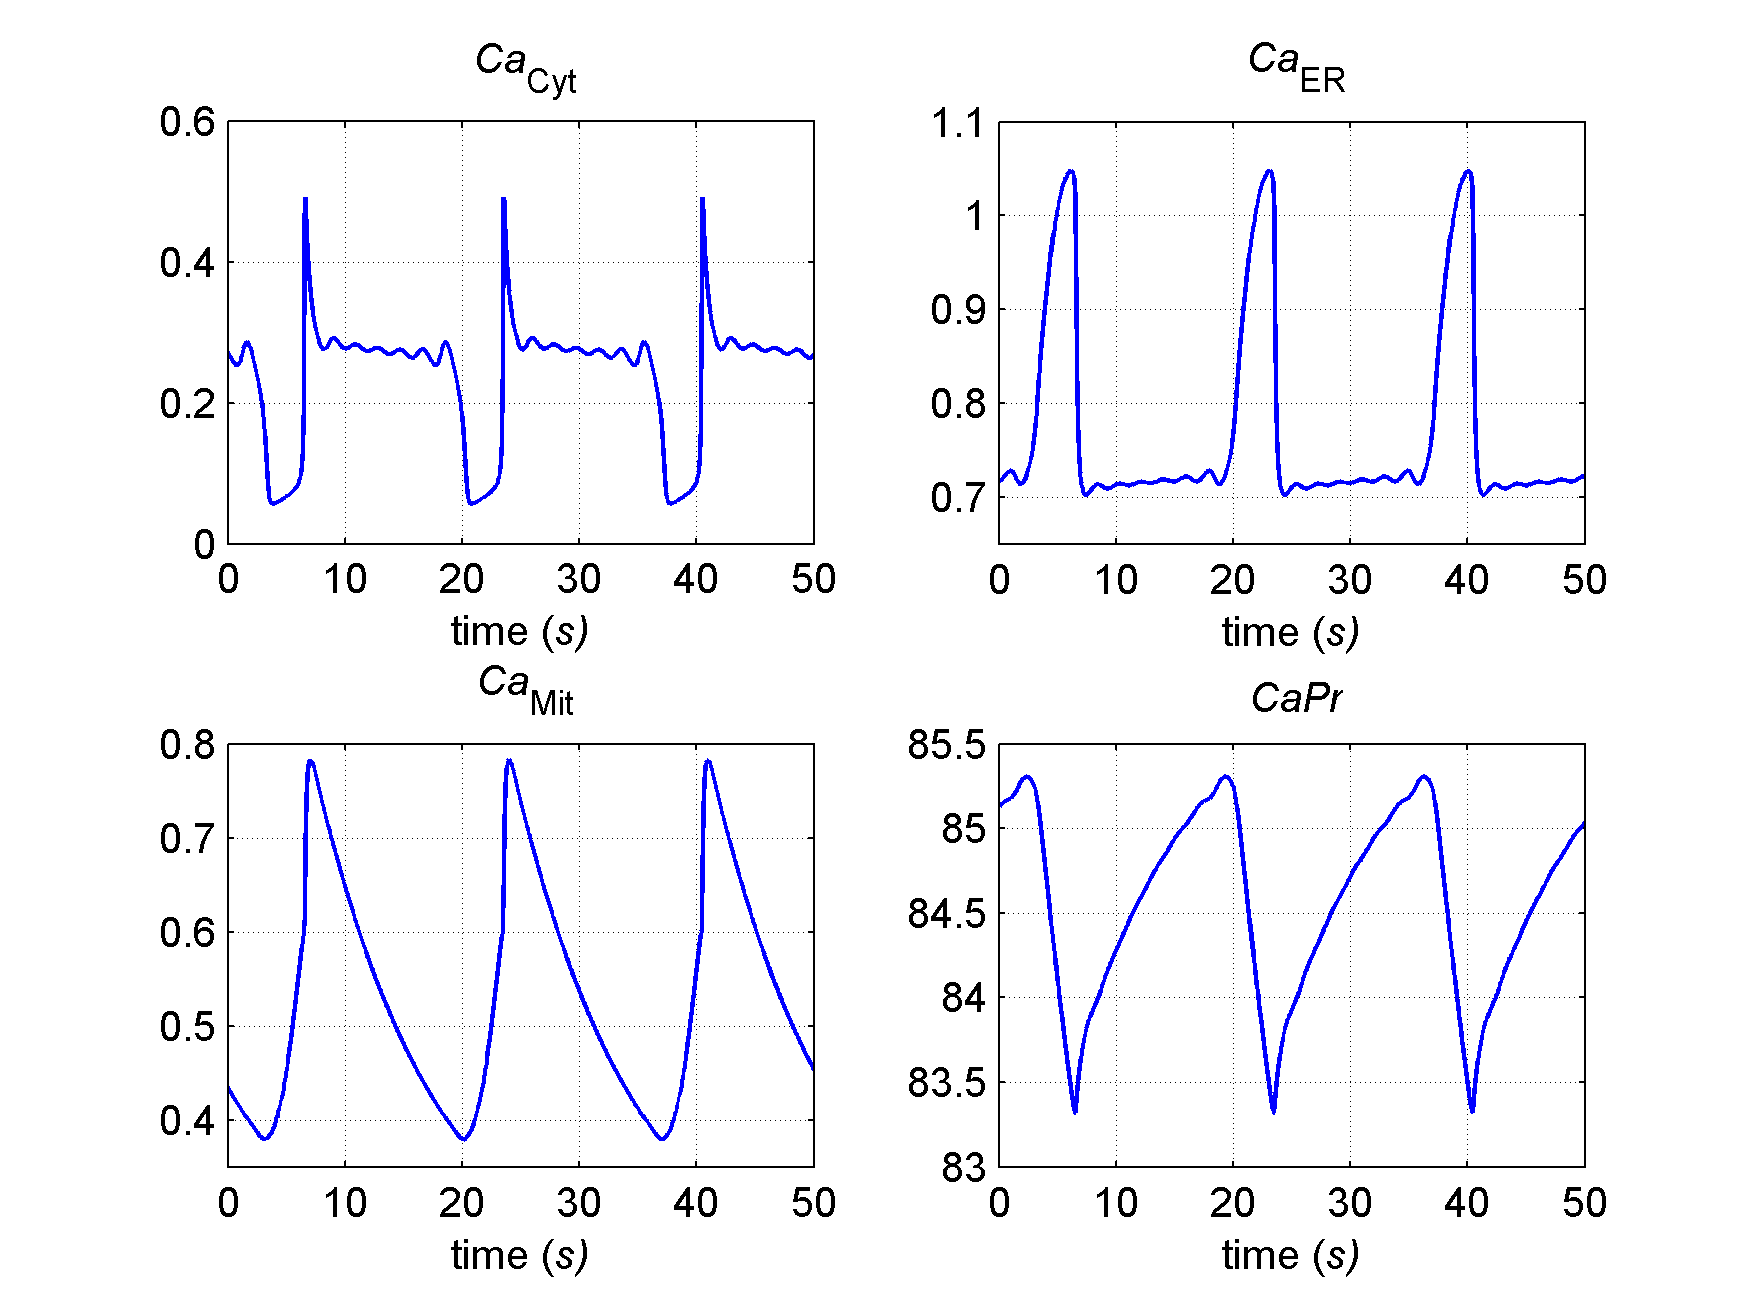
\includegraphics[width=1\textwidth]{rysunki/rozdzial_5/bursting_timecourseMo1}
	\caption[Oscylacje wapniowe typu bursting w Modelu \#1]{Przebiegi czasowe stężeń wolnych jonów  wapnia w poszczególnych kompartmentach  dla  parametrów tak jak w Tab.~\ref{tab:constantsMo1}.}
	\label{fig:complexoscillationsMo1}
\end{figure}

\begin{figure}[ht]
	\centering
	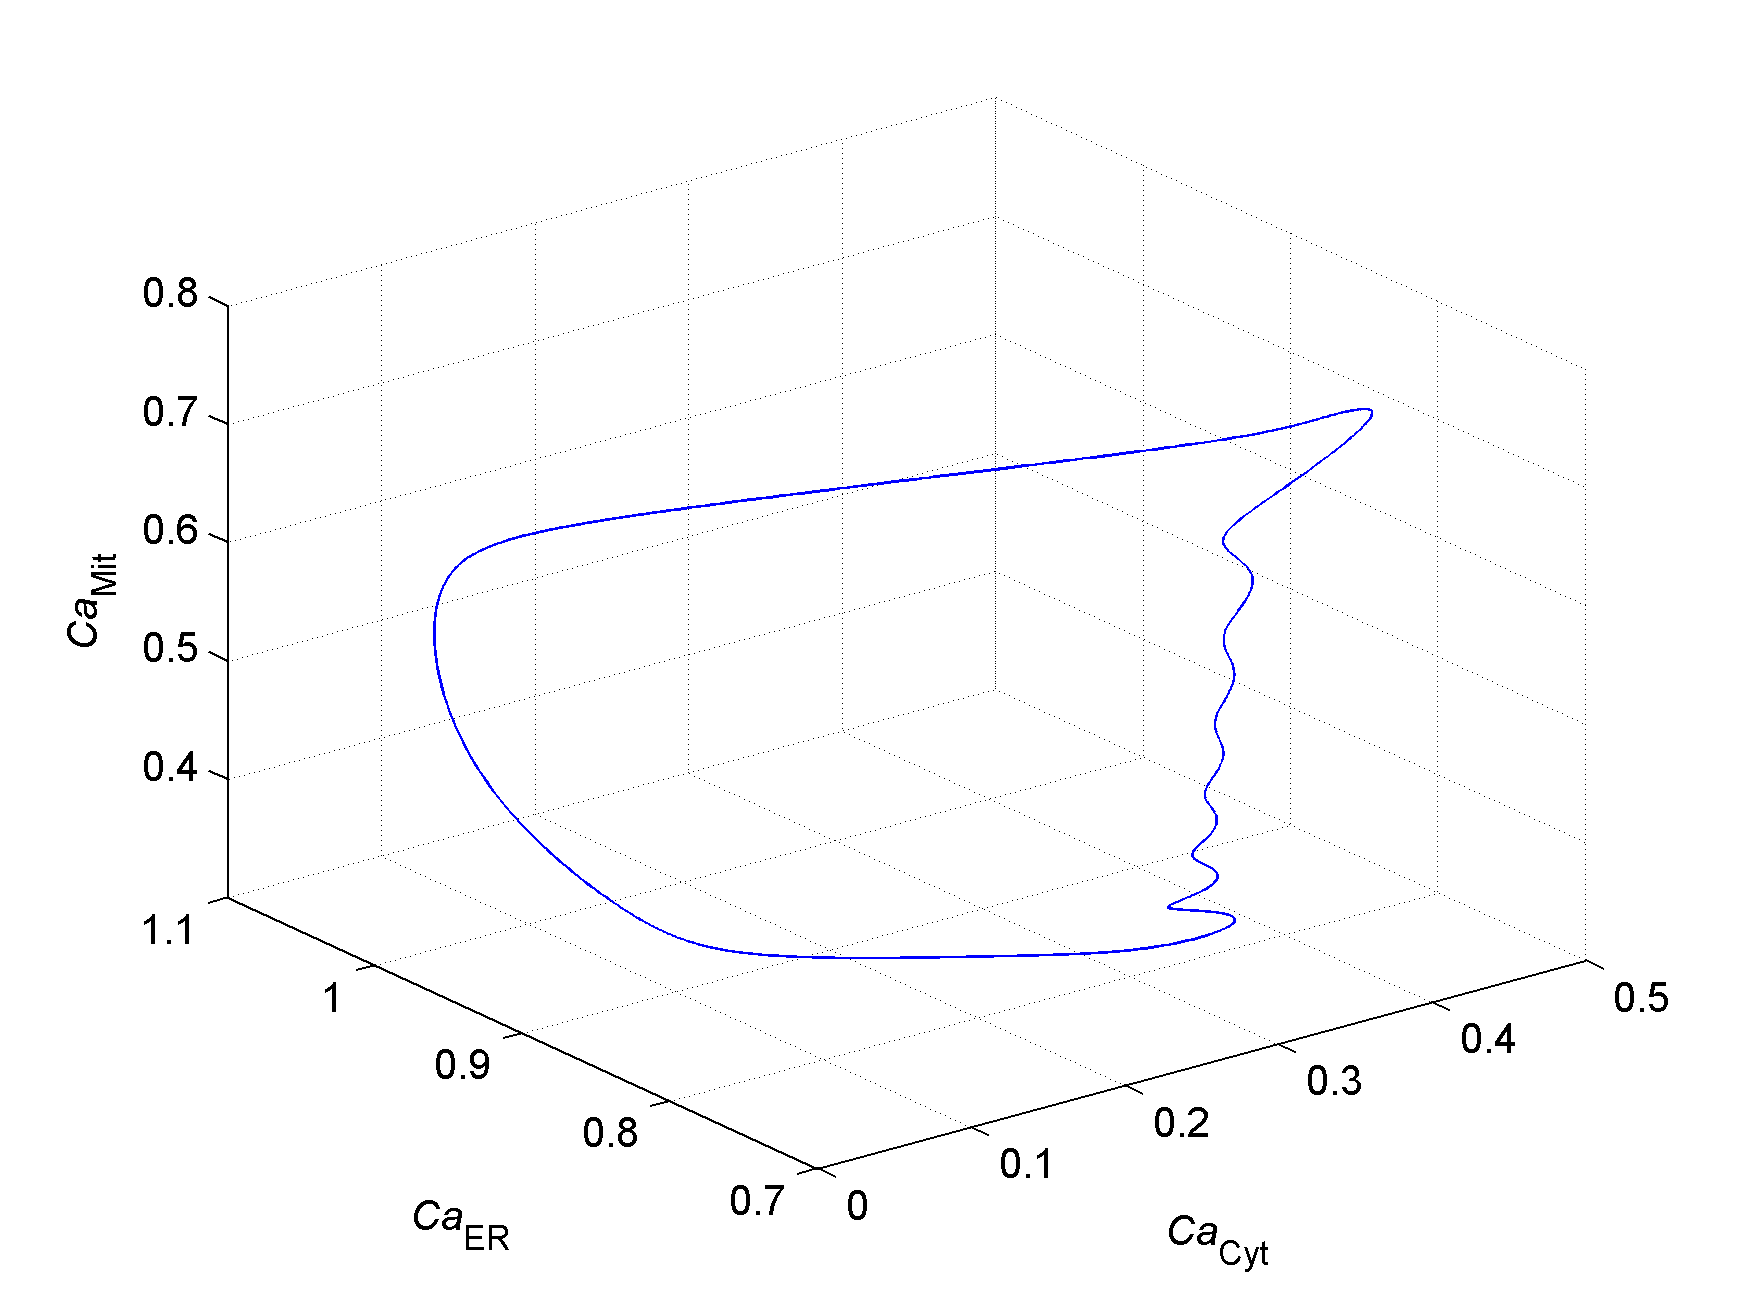
\includegraphics[width=1\textwidth]{rysunki/rozdzial_5/bursting_cycleMo1}
	\caption[Portret fazowy 3-D w Modelu \#1- oscylacje bursting]{Portret fazowy oscylacji typu ,,bursting''. Wszystkie parametry tak jak w~Tab.~\ref{tab:constantsMo1}}
	\label{fig:phaseportraitcomplexMo1}
\end{figure}

Jak widać na Ryc.~\ref{fig:complexoscillationsMo1} oscylacje te mają nieregularny charakter. Dla tego typu oscylacji charakterystyczna jest obecność dwóch składowych w ramach jednego okresu: nagły skok stężenia jonów wapnia (tzw. pik) oraz następujący po nim szereg oscylacji o~wyższej częstotliwości i znacznie mniejszej amplitudzie, niż poprzedzający je wyrzut jonów wapnia. Całkowity okres powyższych oscylacji wynosi $T= 17.1$ s. Stężenia jonów wapnia (w $\mu$M)  w poszczególnych kompartmentach zawierają się w przedziałach: (0.057, 0.49) dla $Ca_{Cyt}$, (0.38, 0.78) dla $Ca_{Mit}$ oraz (0.7, 1.05) dla $Ca_{ER}$. Stężenie wapnia zbuforowanego $CaPr$ zawiera się w przedziale (83.3, 85.3). Przebiegi czasowe stężeń wolnych jonów wapnia w kompartmentach (pierwsze 3 panele na Ryc.~\ref{fig:complexoscillationsMo1}) mogą być odzwierciedlone w zwarty sposób w postaci zamkniętej krzywej w przestrzeni fazowej. Krzywa ta sparametryzowana jest czasem i nosi nazwę stabilnego cyklu granicznego. Cykl graniczny widoczny na Ryc.~\ref{fig:phaseportraitcomplexMo1} posiada wyraźny element o helikalnym kształcie obrazujący, wspomnianą powyżej, drugą składową oscylacji typu ,,bursting''. Składowa ta (o wysokiej częstotliwości i niskiej amplitudzie) jest wynikiem powolnego wypływu jonów wapnia z przedziału mitochondrialnego oraz szybkich procesów wymiany jonów wapnia pomiędzy cytozolem i ER wraz z reakcjami buforowania jonów wapnia przez białka cytozoliczne i retikularne. Okazuje się jednak, że dla innych wartości  parametrów (w~szczególności dla innych wielkości współczynnika $k_{MAM}$ określającego wielkość prądu przez interfejs MaM) oscylacje opisywane układem równań (\ref{eq:1a})--(\ref{eq:3a}) mogą zmienić swój charakter.

\FloatBarrier
\subsubsection*{Oscylacje regularne}

Na Rycinach \ref{fig:regularoscillationsMo1}~i~\ref{fig:phaseportraitregularMo1} przedstawiono \emph{regularne} oscylacje stężenia jonów wapnia w~poszczególnych  kompartmentach oraz obraz cyklu granicznego w przestrzeni fazowej $Ca_{Cyt}$, $Ca_{Mit}$, $Ca_{ER}$.

 
%\noindent Wykresy te pokrywają się z danymi eksperymentalnymi \cite{Berridge1988,Gray1988,Jacob1988}. 

Rycina~\ref{fig:regularoscillationsMo1} przedstawia przebiegi czasowe stężenia jonów wapnia przy zmienionych w stosunku do Tab.~\ref{tab:constantsMo1} współczynnikach $K_2=1.37$ oraz $k_{MAM}=1600$. Oscylacje te maja charakter regularny. Okres oscylacji $T$ wynosi 10.9 s, natomiast stężenia jonów wapnia  w poszczególnych kompartmentach zawierały się w przedziałach: (0.056, 0.56) dla $Ca_{Cyt}$, (0.4, 0.95) dla $Ca_{Mit}$, (0.7, 1.03) dla $Ca_{ER}$, natomiast ilość wapnia zbuforowanego $CaPr$ zawierała się w przedziale (82, 85.25). Jak łatwo zauważyć brak jest tutaj komponenty o podwyższonej ,,częstotliwości'', która występuje w przypadku oscylacji typu ,,bursting'' (Ryc.~\ref{fig:complexoscillationsMo1}). Zwiększenie  przepływu $J_{MAM}$ (poprzez podwyższenie wartości współczynnika $k_{MAM}$ od wartości 1200, jak na Ryc.~\ref{fig:complexoscillationsMo1}, do wartości 1600) spowodowało regularyzację oscylacji stężenia jonów wapnia. Dokładniej wpływ współczynnika $k_{MAM}$ na charakter oscylacji stężeń jonów wapnia oraz istnienie rozwiązań chaotycznych opisany został w podrozdziale~\ref{ss:oscChaotyczne}.

\begin{figure}[ht]
	\centering
	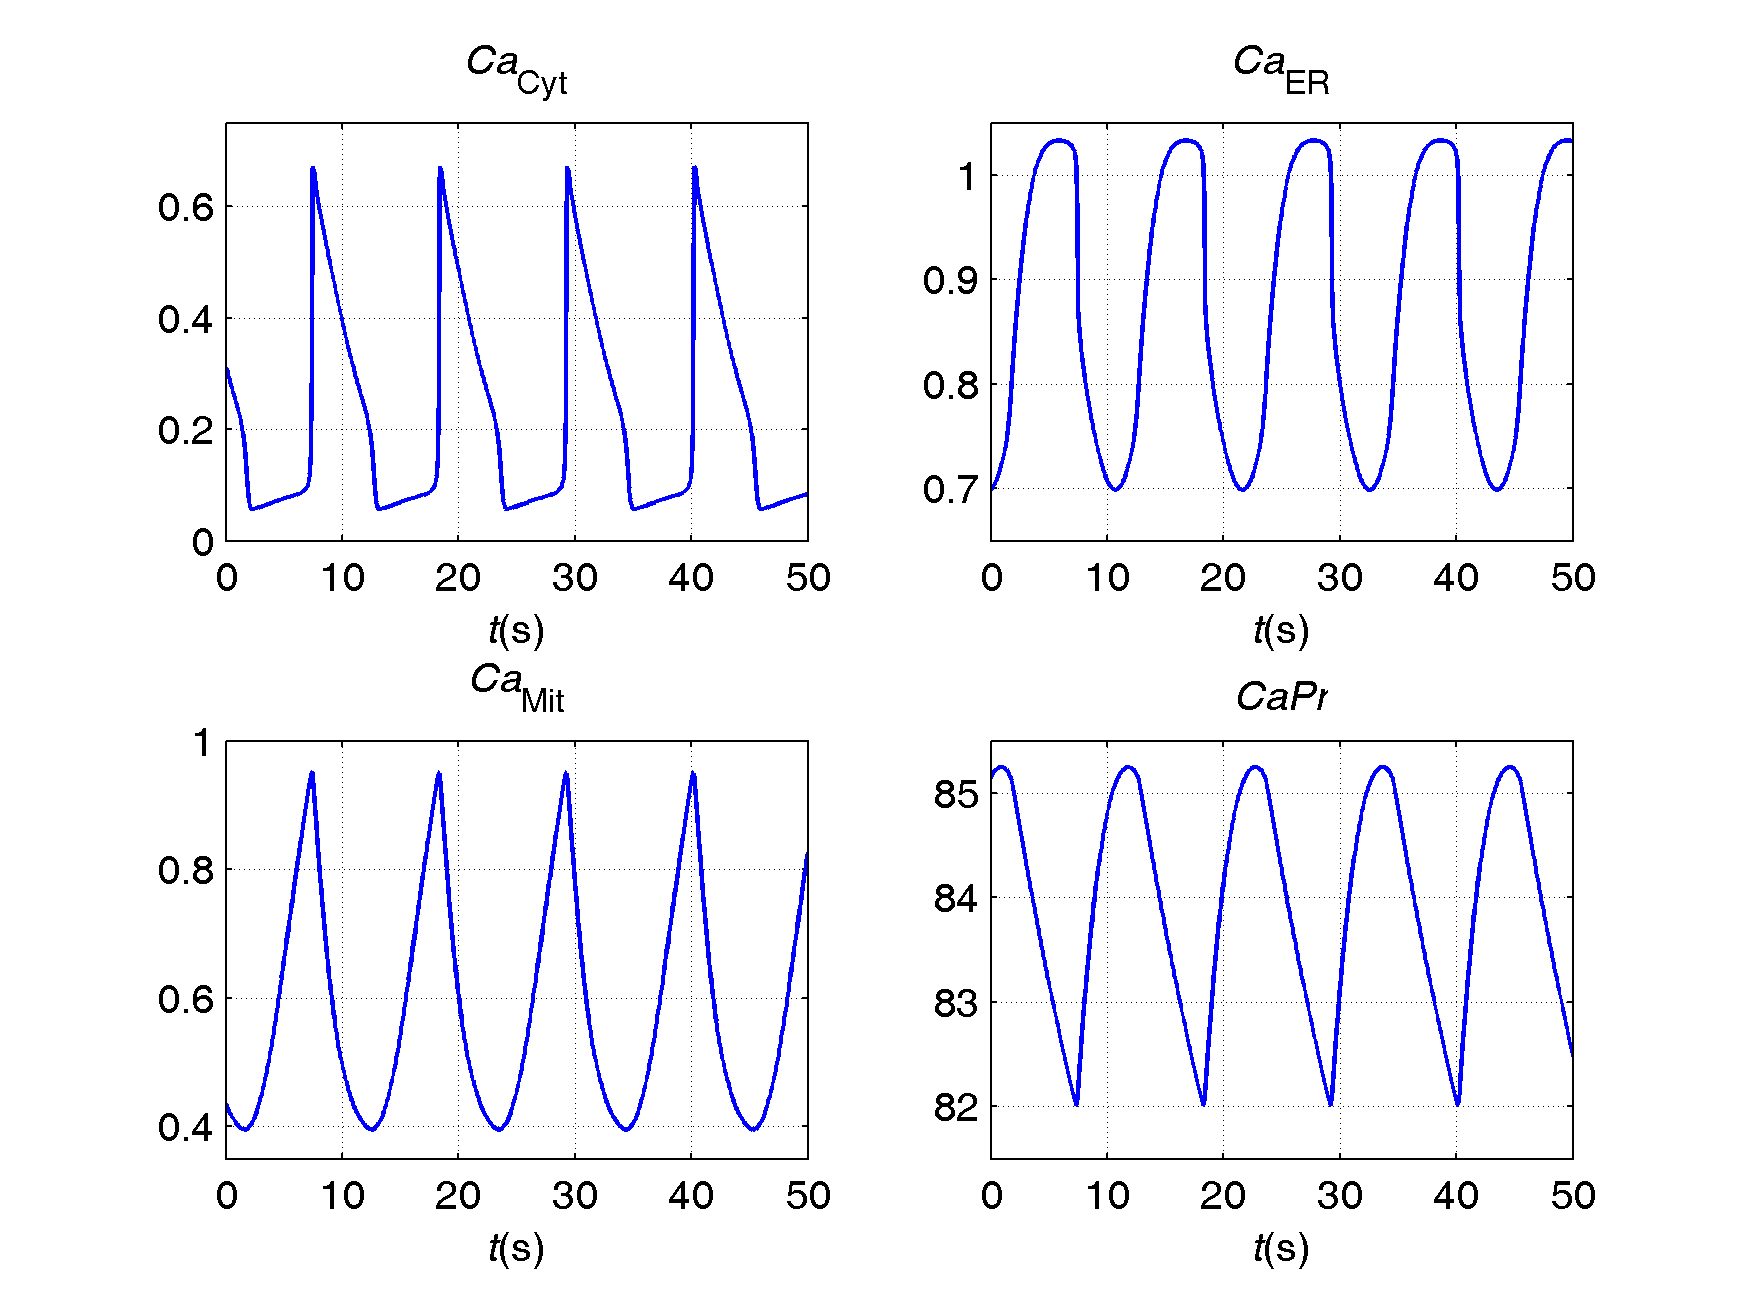
\includegraphics[width=1\textwidth]{rysunki/rozdzial_5/regular_timecourseMo1}
	\caption[Regularne oscylacje wapniowe w Modelu \#1]{Regularne oscylacje wapniowe dla układu równań (\ref{eq:1a})--(\ref{eq:3a}). Parametry: $k_{MAM} = 1600$, $K_{2} = 1.37$ pozostałe parametry jak w Tab.~\ref{tab:constantsMo1}. Wartości stężeń jonów  na  osi pionowej wyrażone w~$\mu$M.}
	\label{fig:regularoscillationsMo1}
\end{figure}

\begin{figure}[ht]
	\centering
	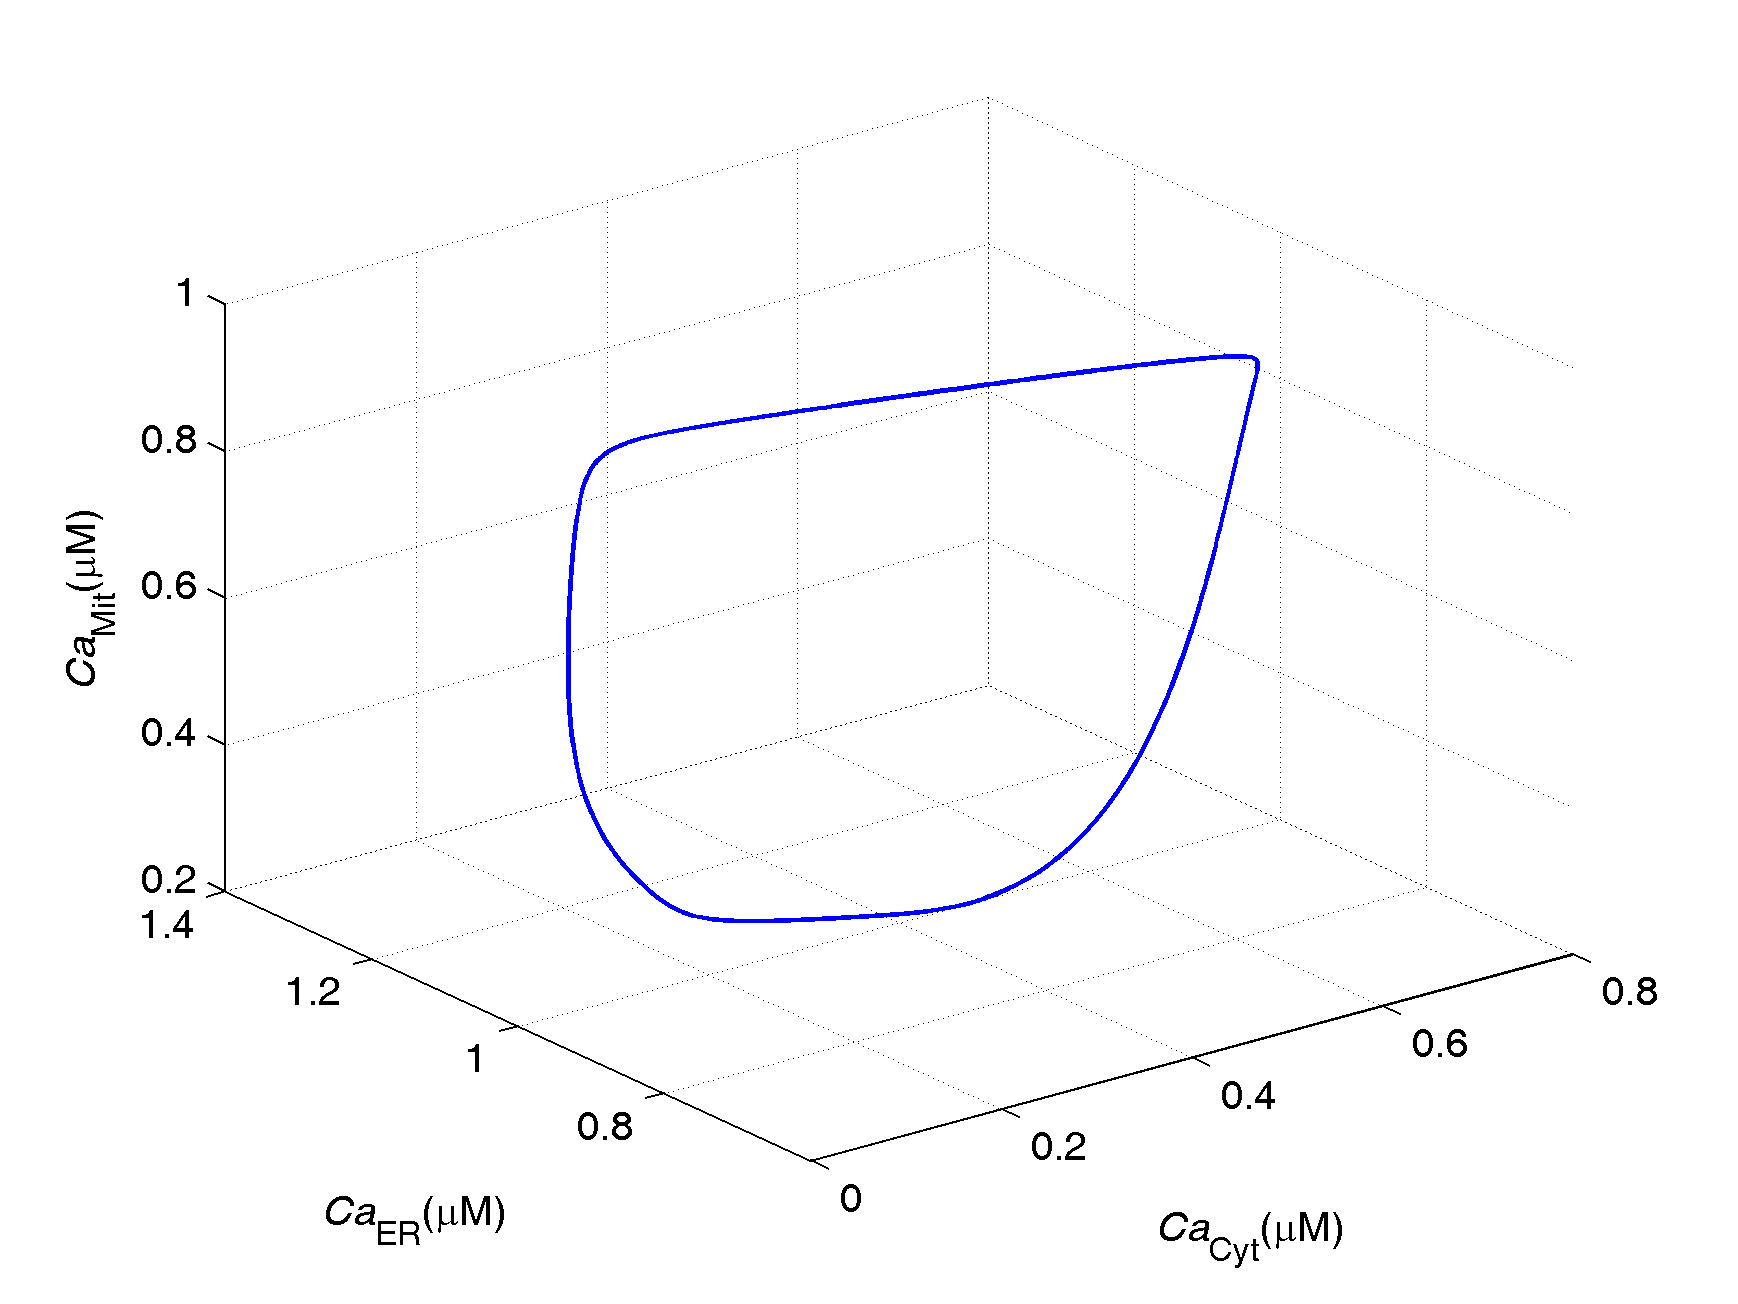
\includegraphics[width=1\textwidth]{rysunki/rozdzial_5/regular_cycleMo1}
	\caption[Portret fazowy w Modelu \#1 - oscylacje regularne]{Portret fazowy oscylacji regularnych oscylacji wapniowych dla układu równań (\ref{eq:1a})--(\ref{eq:3a}) dla następującego zestawu parametrów $k_{MAM} = 1600$, $K_{2} = 1.37$ pozostałe parametry jak w~Tab.~\ref{tab:constantsMo1}.}
	\label{fig:phaseportraitregularMo1}
\end{figure}

\FloatBarrier
\subsubsection*{Analiza pojedynczego cyklu oscylacji typu ,,bursting''}

Pojedynczy okres oscylacji nieregularnych typu ,,bursting'', odpowiadający panelom z Ryc.~\ref{fig:complexoscillationsMo1}, dla zestawu parametrów jak w Tab.~\ref{tab:constantsMo1}, widoczny jest na Ryc.~\ref{fig:jedenOkres}. (Na rycinie przedstawiającej jeden okres druga składowa o niskiej amplitudzie i wysokiej częstotliwości jest słabo widoczna, z uwagi na rozciągniecie osi czasu.) Każdy cykl może być podzielony na trzy fazy. Faza I - zaczyna się gdy poziom wapnia w cytozolu (Ca$_{Cyt}$) osiąga wartość maksymalną ($t = 7.6$~s) i trwa do czasu aż poziom wapnia w mitochondriach (Ca$_{Mit}$) osiągnie wartość maksymalną ($t = 8.1$ s). W tej fazie wiodącymi procesami są: uwalnianie wolnych jonów wapnia z~retikulum oraz znaczny pobór Ca$^{2+}$ przez mitochondria i buforowanie poprzez białka cytozolu. 

\begin{figure}[ht]
	\centering
	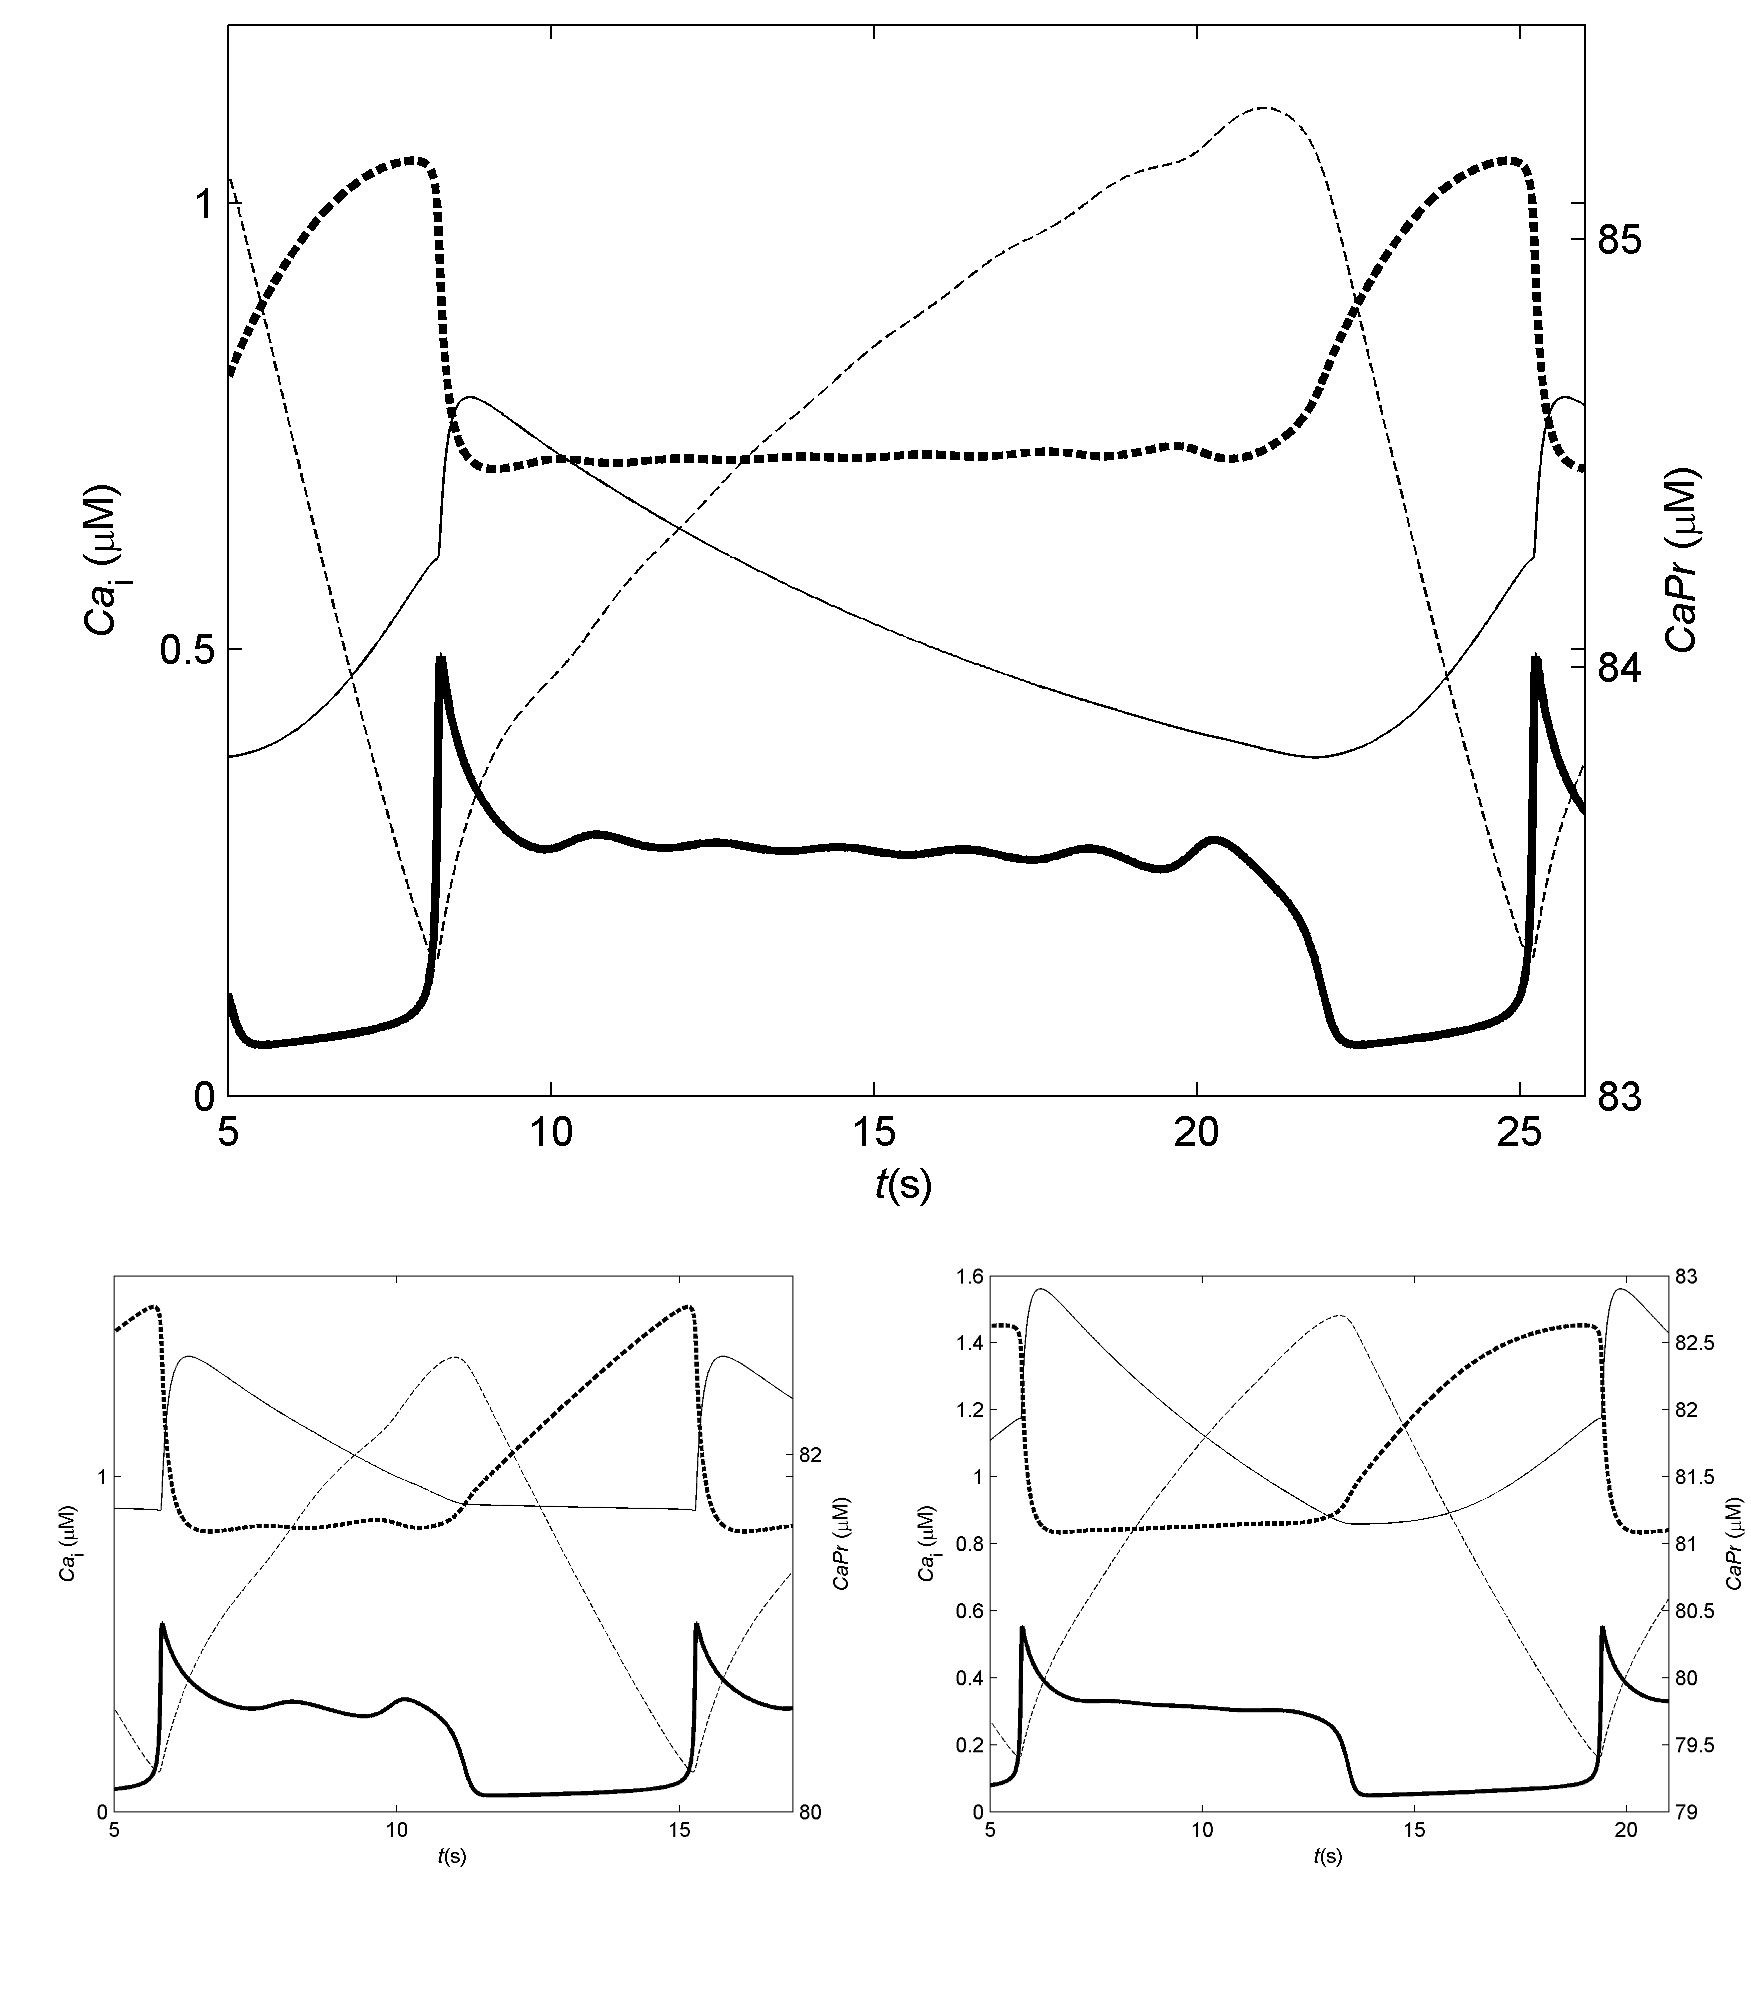
\includegraphics[width=0.9\textwidth]{rysunki/rozdzial_5/one_periodMo1}
	\caption[Analiza pojedynczego okresu w modelu \#1]{Analiza pojedynczego okresu oscylacji stężenia jonów wapnia. $Ca_i$ - oznacza stężenie jonów wapnia w i-tym kompartmencie. $CaCyt$ - pogrubiona, pełna linia; $CaMit$ - cienka, pełna linia; $CaER$ - pogrubiona, przerywana linia; $CaPr$ - cienka, przerywana linia. Stężenie buforów wapniowych $Pr$ do $CaPr$ wynika z równania \ref{eq:cons:Ca} i nie zostało ujęte na powyższym wykresie. Parametry dla górnego panelu tak jak w~Tab.~\ref{tab:constantsMo1}; dolny lewy panel: $k_{ch} = 2950$, $k_{MAM} = 3$; dolny prawy panel:  $k_{ch} = 2950$, $k_{MAM} = 87$.}
	\label{fig:jedenOkres}
\end{figure}

W fazie drugiej aktywowany jest powolny strumień wapnia z mitochondriów do cytozolu. Większość uwolnionych jonów wapnia związana jest z cytozolicznymi białkami buforującymi. Ważnym procesem, zachodzącym w tej fazie jest szybka wymiana wapnia pomiędzy cytozolem i ER, co prowadzi do małych, szybkich drgań stężenia wapnia w~tych kompartmentach (wspomniana powyżej druga składowa oscylacji). Ten etap kończy się, gdy poziom wapnia buforowanego ($CaPr$) osiąga wartość maksymalną (tj. dla $t = 20.7$ s).

W fazie III, wiodącym procesem jest dysocjacja kompleksów białkowo-wapniowych. Mitochondria i ER są "ładowane", podczas gdy poziom wapnia w cytozolu najpierw zmniejsza się, a następnie wzrasta, aby osiągnąć maksymalną wartość, którą jest koniec III fazy ($t = 24.7$ s). 

\FloatBarrier
\subsection{Wpływ $k_{MAM}$ na charakter oscylacji stężenia jonów wapnia}
\label{ss:oscChaotyczne}

Na Ryc.~\ref{fig:chaos_fazowyMo1} widoczne są zmiany stężenia jonów wapnia w cytozolu i w mitochondriach dla $k_{ch} = 2950$ i $k_{MAM} = 0$, co odpowiada sytuacji, w której przepływ jonów wapnia przez te struktury został w tym przypadku całkowicie pominięty. 

\begin{figure}[ht!]
\centering
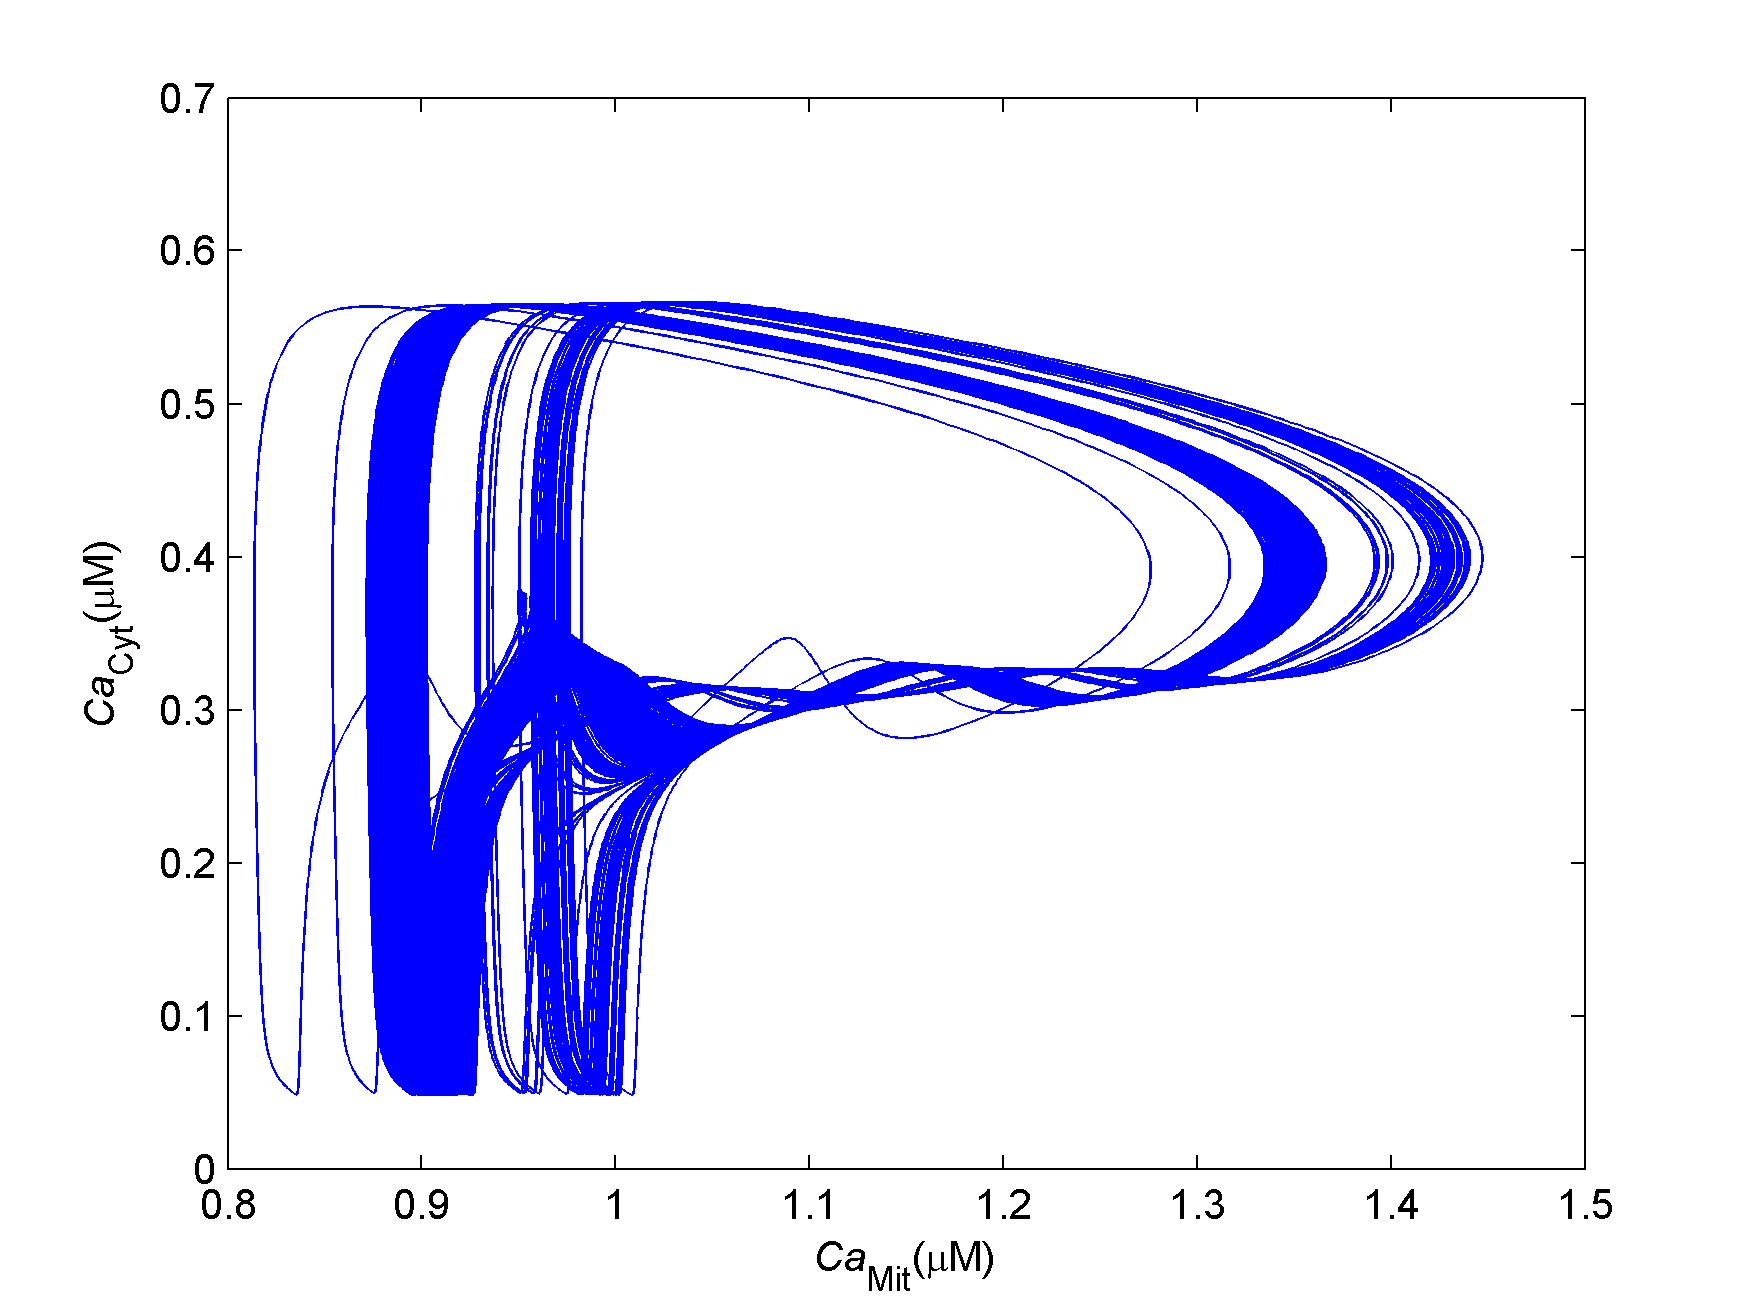
\includegraphics[width=0.9\textwidth]{rysunki/rozdzial_5/marhl_chaos}
\caption[Oscylacje chaotyczne w Modelu \#1 - portret fazowy]{Portret fazowy oscylacji o charakterze chaotycznym dla parametrów $k_{ch} = 2950$ i $k_{MAM}=0$.}
\label{fig:chaos_fazowyMo1}
\end{figure}


\begin{figure}[ht!]
	\centering
	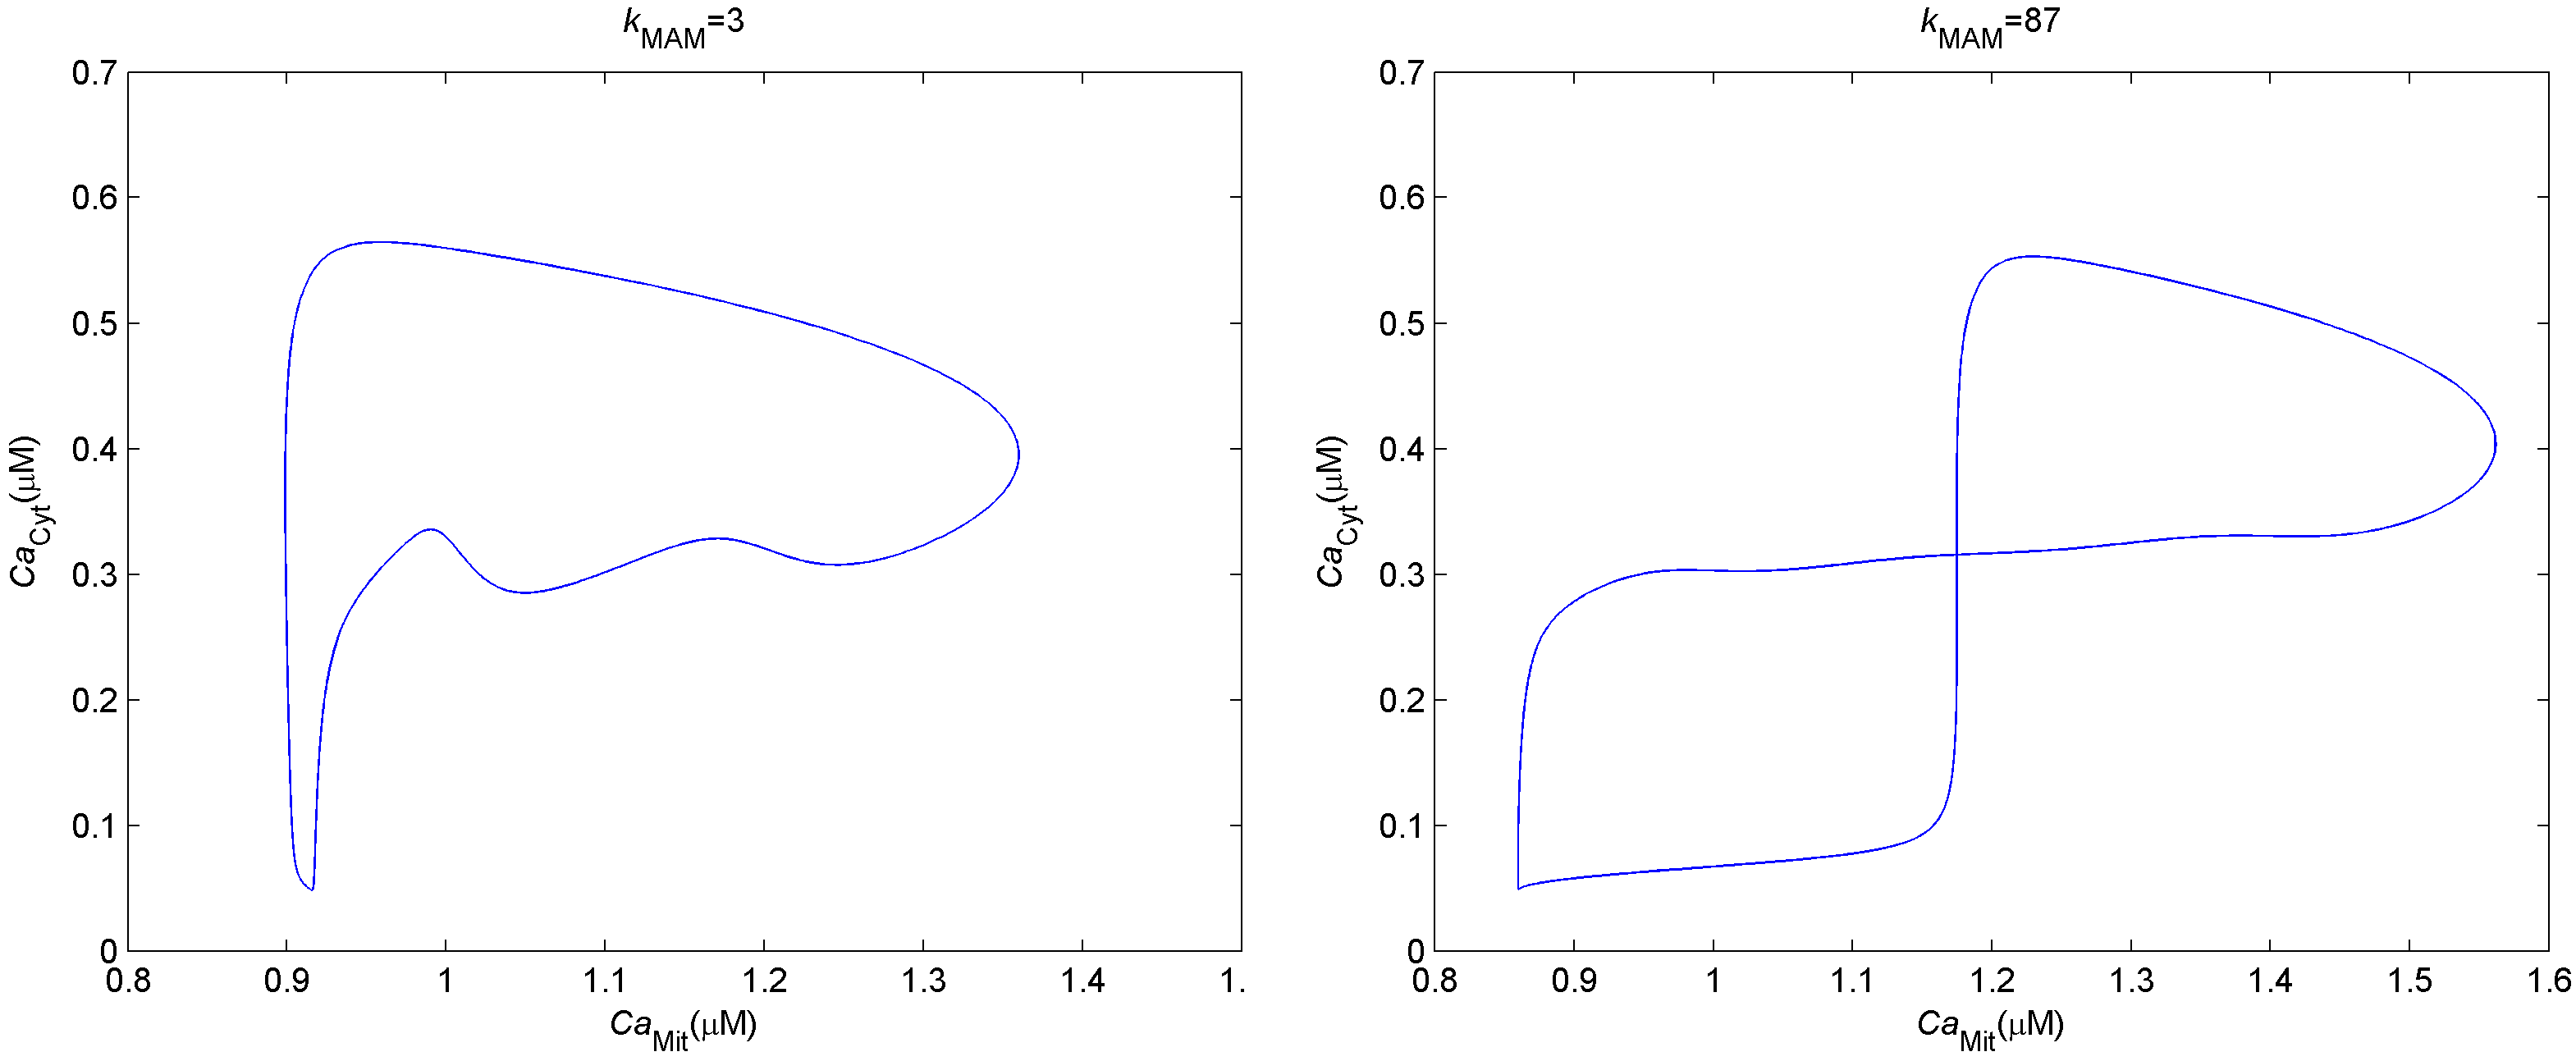
\includegraphics[width=0.9\textwidth]{rysunki/rozdzial_5/marhl_chaos_Kmam-3}
	\caption[Rzut trajektorii rozwiązania periodycznego]{Rzut trajektorii rozwiązania periodycznego (cyklu granicznego) na płaszczyznę $Ca_{Cyt}$ -- $Ca_{Mit}$, $Ca_{ER}$ dla $k_{ch}=2950$. Lewy panel $k_{MAM}=3$, prawy panel $k_{MAM}=87$.}
	\label{fig:marhlregularyzacja}
\end{figure}


Jak sugeruje Ryc.~\ref{fig:marhlregularyzacja} wprowadzenie nawet niewielkiego przepływu jonów wapniowych przez struktury MAM (przez zadanie niezerowej stałej $k_{MAM}$) powoduje, że oscylacje chaotyczne zanikają. Wprowadzenie przepływu  przez struktury MAM nie tylko regularyzuje przepływy wapniowe w komórce, ma również duży wpływ na kształt profili oscylacji wapniowych. W obu przypadkach, przedstawionych na Ryc.~\ref{fig:marhlregularyzacja} ($k_{MAM} = 3$ oraz $k_{MAM} = 87$) mamy do czynienia z dobrze określonym cyklem granicznym. Dla $k_{MAM} = 3$  rzut cyklu na płaszczyznę $Ca_{Cyt}$ -- $Ca_{Mit}$ składa się z jednej pętli, natomiast dla wartości $k_{MAM} = 87$ rzut cyklu granicznego tworzy krzywą o~ósemkowym kształcie. 

Wzrost współczynnika $k_{MAM}$ powoduje, że pionowa cześć trajektorii z Ryc.~\ref{fig:marhlregularyzacja} (odpowiadająca mechanizmowi szybkiego ładowania cyzolu pod koniec fazy III) przechodzi do obszaru o wyższym stężeniu jonów wapnia w mitochondrium ($\approx$ 1.3 -- 1.6 $\mu$M). Zmienia się zatem mechanizm ładowania mitochondriów. Dla $k_{MAM} = 3$ mamy szybkie ładowanie mitochondriów wraz z szybkim ładowaniem cytozolu. Dla $k_{MAM} = 87$, oprócz szybkiego mechanizmu ładowania cytozolu i mitochondriów, występuje także wolne ładowanie kompartmentu mitochondrialnego, przy bardzo niskim, niemal stałym, poziomie jonów wapnia w cytozolu. Warto zauważyć, że w tej fazie niemal cała pula jonów wapnia, która jest sekwestrowana przez mitochondria i ER, pochodzi z~dysocjacji  kompleksów buforujących wapń.

Jednak wpływ struktur MAM na oscylacje stężenia jonów wapnia jest o wiele bardziej złożony, niż prosta regularyzacja trajektorii. Przeanalizowaliśmy wpływ współczynnika $k_{MAM}$ na trajektorie dla dwóch wartości $k_{ch}$: 2950 oraz 4100, dla których asymptotyczne  zachowanie systemu ($k_{MAM} = 0$) rozwiązań oscylacyjnych  jest odpowiednio chaotyczne lub odpowiada stabilnym rozwiązaniom periodycznym (znaleziono stabilny cykl graniczny). Zaobserwowano szereg rozwiązań stabilnych dla szerokiego zakresu wartości parametru $k_{MAM}$. Dla $k_{ch}$ równego 2950 wartości $k_{MAM}$ były brane z~przedziału (0,101), natomiast dla $k_{ch}$ równego 4100 wartości $k_{MAM}$ były brane z~przedziału (0,1600). W zależności od wartości parametru $k_{MAM}$ uzyskaliśmy różne rodzaje rozwiązań periodycznych (cykli granicznych o różnej ,,krotności'' - Ryc.~\ref{fig:jakosciowy}) oraz oscylacyjne rozwiązania o charakterze chaotycznym. Rozwiązanie uznawaliśmy za stabilne jeśli najwyższy wykładnik Lapunowa wynosił 0, a pozostałe dwa były ujemne. Rozwiązanie uznawaliśmy za chaotyczne jeśli jeden z wykładników przyjmował wartość 0, natomiast pozostałe dwa były niezerowe i miały rózny znak. Np. dla $k_{ch}=2950$ i~$k_{MAM}=30$ wykładniki Lapunowa wynoszą odpowiednio: $\lambda_1=8.9 \times 10^{-6}$ (odpowiadająca wykładnikowi zerowemu), $\lambda_2=-0.07$ oraz $\lambda_3=-4.54$. Zakres czasowy dla analizowanych trajektorii wynosił 5000 s, z kolei krok czasowy dla ortonormalizacji  Gramma-Schmidta wybrano na 2~s. Wykładniki Lapunowa zostały obliczone za pomocą pakietu MATDS dla systemu MATLAB do badań systemów dynamicznych \cite{Govorukhin2009}. Numeryczne wyznaczenie wykładników Lapunowa obarczone jest często relatywnie dużym błędem, który spowodowany jest trudnym doborem odpowiedniego kroku czasowego ortonormalizacji Gramma-Schmidta. Dlatego też dość często mieliśmy do czynienia z sytuacją, w której niezerowe wykładniki Lapunowa miały różny znak, lecz bardzo małą wartość (rzędu $10^{-5}$), co uniemożliwiało prawidłową klasyfikację trajektorii. W takich przypadkach, aby zdecydować, czy trajektoria jest chaotyczna, czy też jest cyklem granicznym (jedno- lub wielokrotnym), wyznaczane były przekroje Poincar\'ego i szacowany wymiar korelacji $D_2$ atraktora. Do obliczeń używaliśmy pakietu Tisean \cite{Hegger1999,Kantz2004}. Przekroje  Poincar\'ego w płaszczyźnie Ca$_{Mit}=1.2$ (lewy panel) i~szacowany wymiar korelacji dla trajektorii chaotycznej dla parametrów $k_{ch}=2950$, $k_{MAM}=73$ (prawy panel) są przedstawione na Ryc.~\ref{fig:returnmap}. Ponieważ punkty przecięcia trajektorii z płaszczyzną przekroju tworzą rozmyty łuk, sugeruje to, że badana trajektoria jest chaotyczna \cite{Ozer2005}. W przypadku cyklu granicznego zbiór punktów skupienia w jego przekroju Poincar\'ego byłby jednym lub kilkoma punktami, w zależności od stopnia jego komplikacji. Przekrój Poincar\'ego znacznie upraszcza analizę skomplikowanych trajektorii okresowych lub quaziokresowych, zachowując jednocześnie istotne informacje na temat jego dynamiki.

\begin{figure}[!ht]
	\centering
	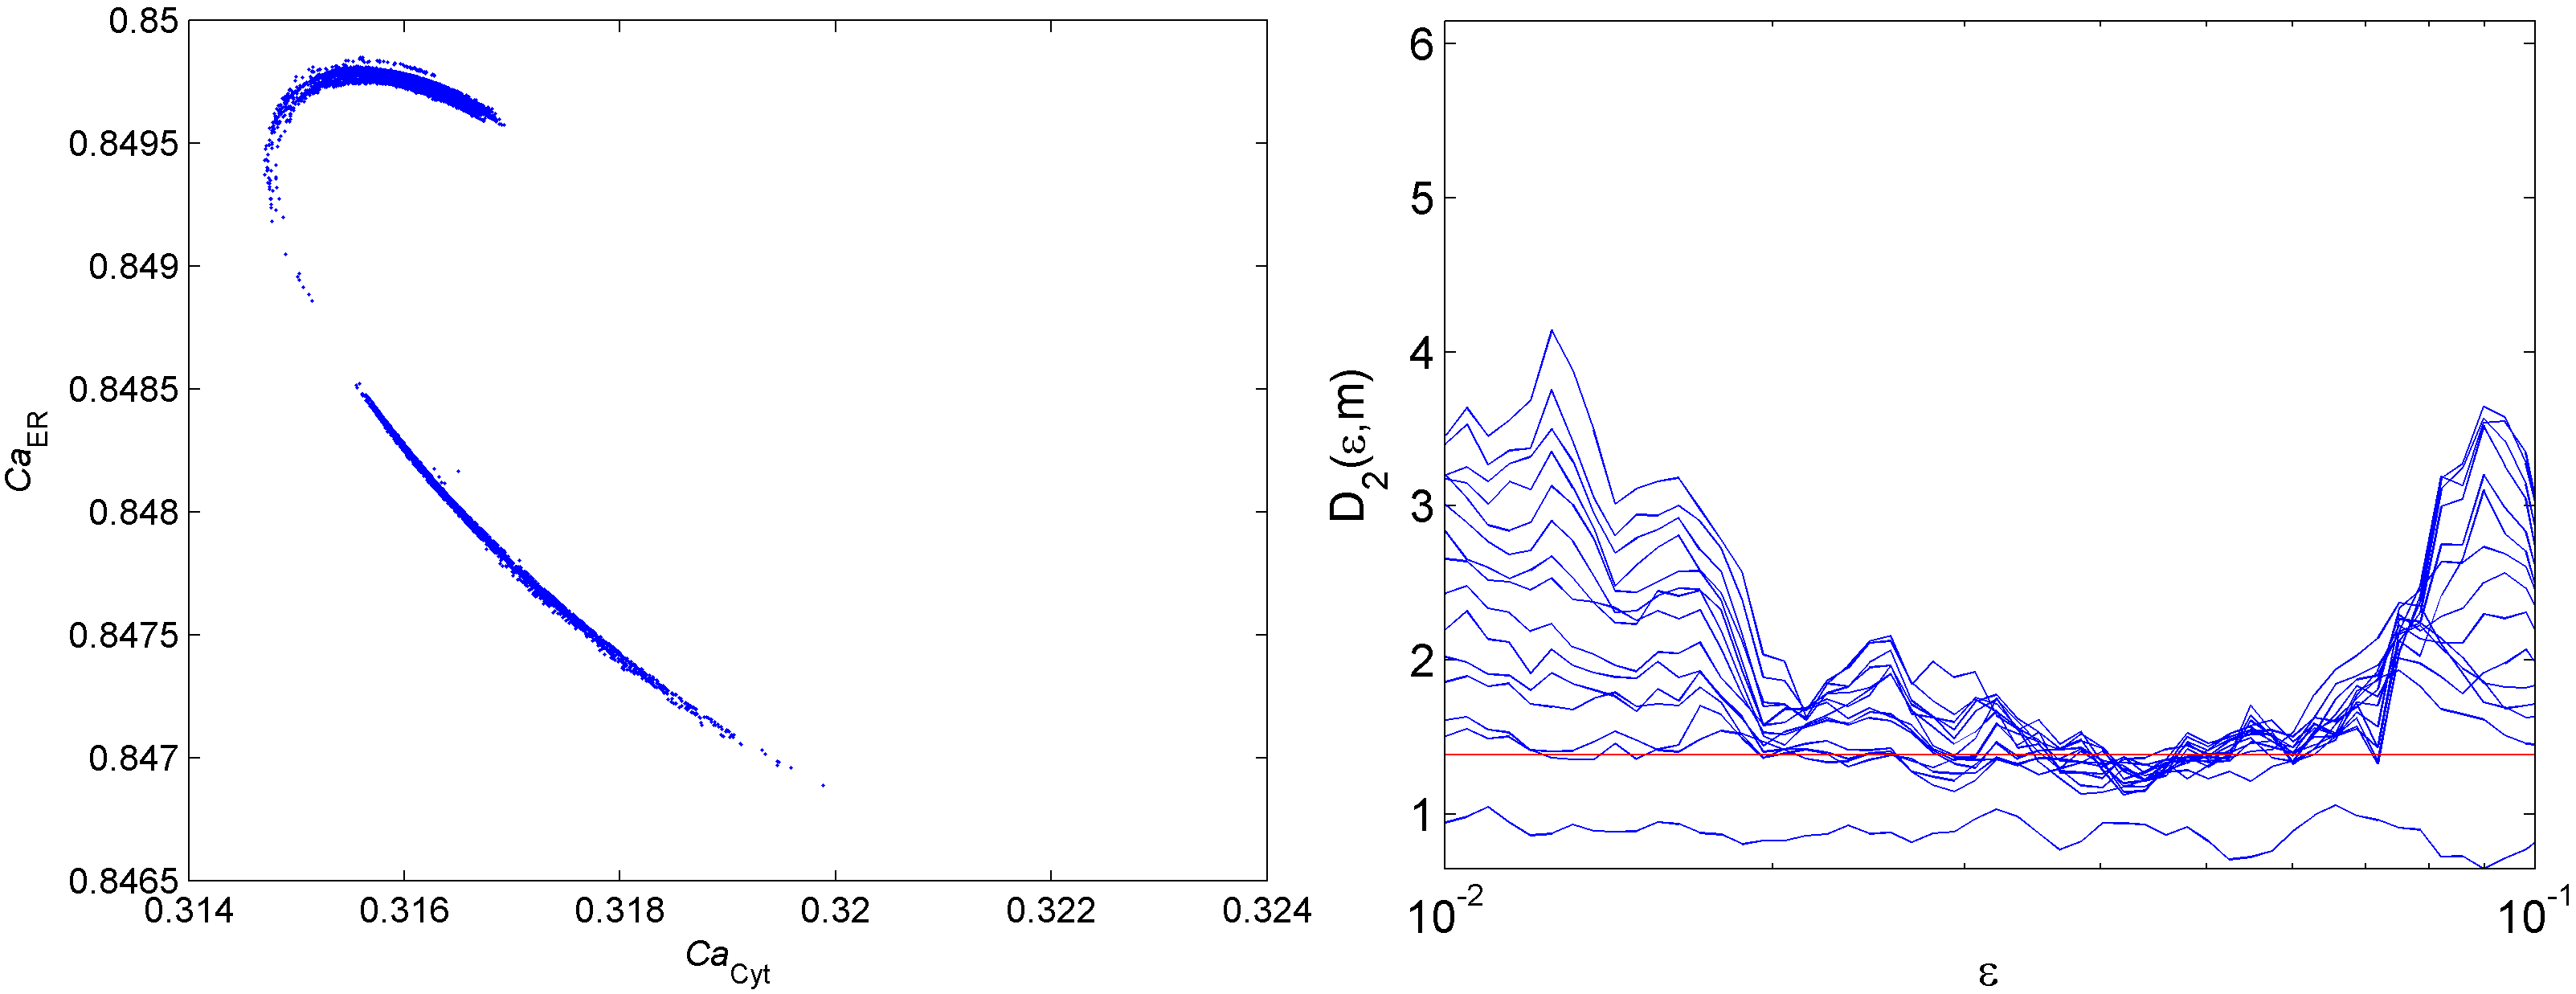
\includegraphics[width=1\textwidth]{rysunki/rozdzial_5/kmam73_all}
	\caption[Przekroje Poincar\'ego w Modelu \#1]{Lewy panel: przekroje Poincar\'ego  w płaszczyźnie $\textrm{Ca}_{Mit}=1.2$. Parametry jak w Tab.~\ref{tab:constantsMo1} za wyjątkiem $k_{ch}=2950$ oraz $k_{MAM} = 73$. Prawy panel: lokalne nachylenia sum korelacyjnych dla różnych wymiarów włożenia $m$ (przyporządkowanych poszczególnym krzywym) w zależności od   wymiaru pudełek $\varepsilon$ - niebieskie linie. Oszacowany wymiar korelacji $D_2=1.34$ - czerwona linia (parametry jak w Tab.~\ref{tab:constantsMo1}).}
	\label{fig:returnmap}
\end{figure}

\bigskip

Szacunkowy wymiar korelacji $D_2$ (w notacji stosowanej przez \cite{Hegger1999}) dla różnych wartości parametru $k_{MAM} $ i parametru $k_{ch} = 2950$ przedstawiono w Tab.~\ref{tab:dimensions}.

\bigskip

\begin{table}[!h]
	\centering
	\begin{tabular}{|l|c|c|c|c|c|c|c|c|c|} \hline
		\rule{0pt}{4ex}$k_{MAM}$	&0	&	41		&	42		&	43		&  46	& 68	& 72	& 73	& 89	\\[1.8ex] \hline
		\rule{0pt}{4ex}$D_2$		 & 1.84	&1.02	&	1.05	&	1.12	& 1.64	& 1.1	& 1.02	& 1.34	& 1.09	\\[2ex] \hline
	\end{tabular}
	\caption [Korelacja wymiaru atraktorów]{Korelacja wymiarów atraktorów dla $k_{ch} = 2950$.} 
	\label{tab:dimensions}
\end{table} 

	Dokładniejsza  analiza zachowań rozwiązań modelu wykonana dla parametru  $k_{ch} = 2950$ oraz parametru $k_{MAM}$ w przedziale 0--200, z krokiem równym 1 wykazała, że zmiana wartości $k_{MAM}$ w znacznym stopniu zmieniała rodzaj uzyskanych oscylacji stężeń jonów wapnia (Ryc.~\ref{fig:jakosciowy}). Dla $k_{MAM}$ z powyższego przedziału zaobserwowaliśmy 1-, 2-, 3-, a nawet 7-krotne cykle graniczne oraz oscylacje o charakterze chaotycznym. Pojedyncze cykle graniczne zostały zaobserwowane dla $k_{MAM}$ z zakresów 1--39, 74--75 i 86--88. Podwójne cykle graniczne istnieją dla $k_{MAM}$ z zakresów 47--67, 76--85, 90--94, 96--98, 100--101 oraz $k_{MAM}$=40. Potrójne cykle graniczne występują dla $k_{MAM}$ równego 69 i 70. Ponadto zaobserwowano siedmiokrotny cykl graniczny dla $k_{MAM}=71$. Analiza wykładników Lapunowa i przecięć Poincar\'ego sugerują istnienie występowania chaosu deterministycznego dla  $k_{MAM}$ z przedziałów 41--46, 72--73 i dla $k_{MAM}$ równego 0, 68, 89, 95, 99. Ryc.~\ref{fig:jakosciowy} przedstawia schematycznie uzyskane wyniki dla $k_{MAM}$ z~przedziału od 0--101. Co więcej dla parametru $k_{MAM} \geq 102$ nie uzyskaliśmy stabilnego cyklu granicznego. Dla tych wartości większość trajektorii przyciągana była do stabilnego punktu stacjonarnego z wysokim poziomem jonów wapnia w przedziale mitochondrialnym ($Ca_{Mit}>18 \mu$M) - Ryc.~\ref{fig:steadystatesMo1} - co może zostać uznane za początkową fazę apoptozy, której wewnętrzny szlak inicjuje proces akumulacji jonów wapnia w~mitochondrium \cite{Hajnoczky2006,Joseph2007,Roy2008}.

\begin{sidewaysfigure}[p]
	\centering
	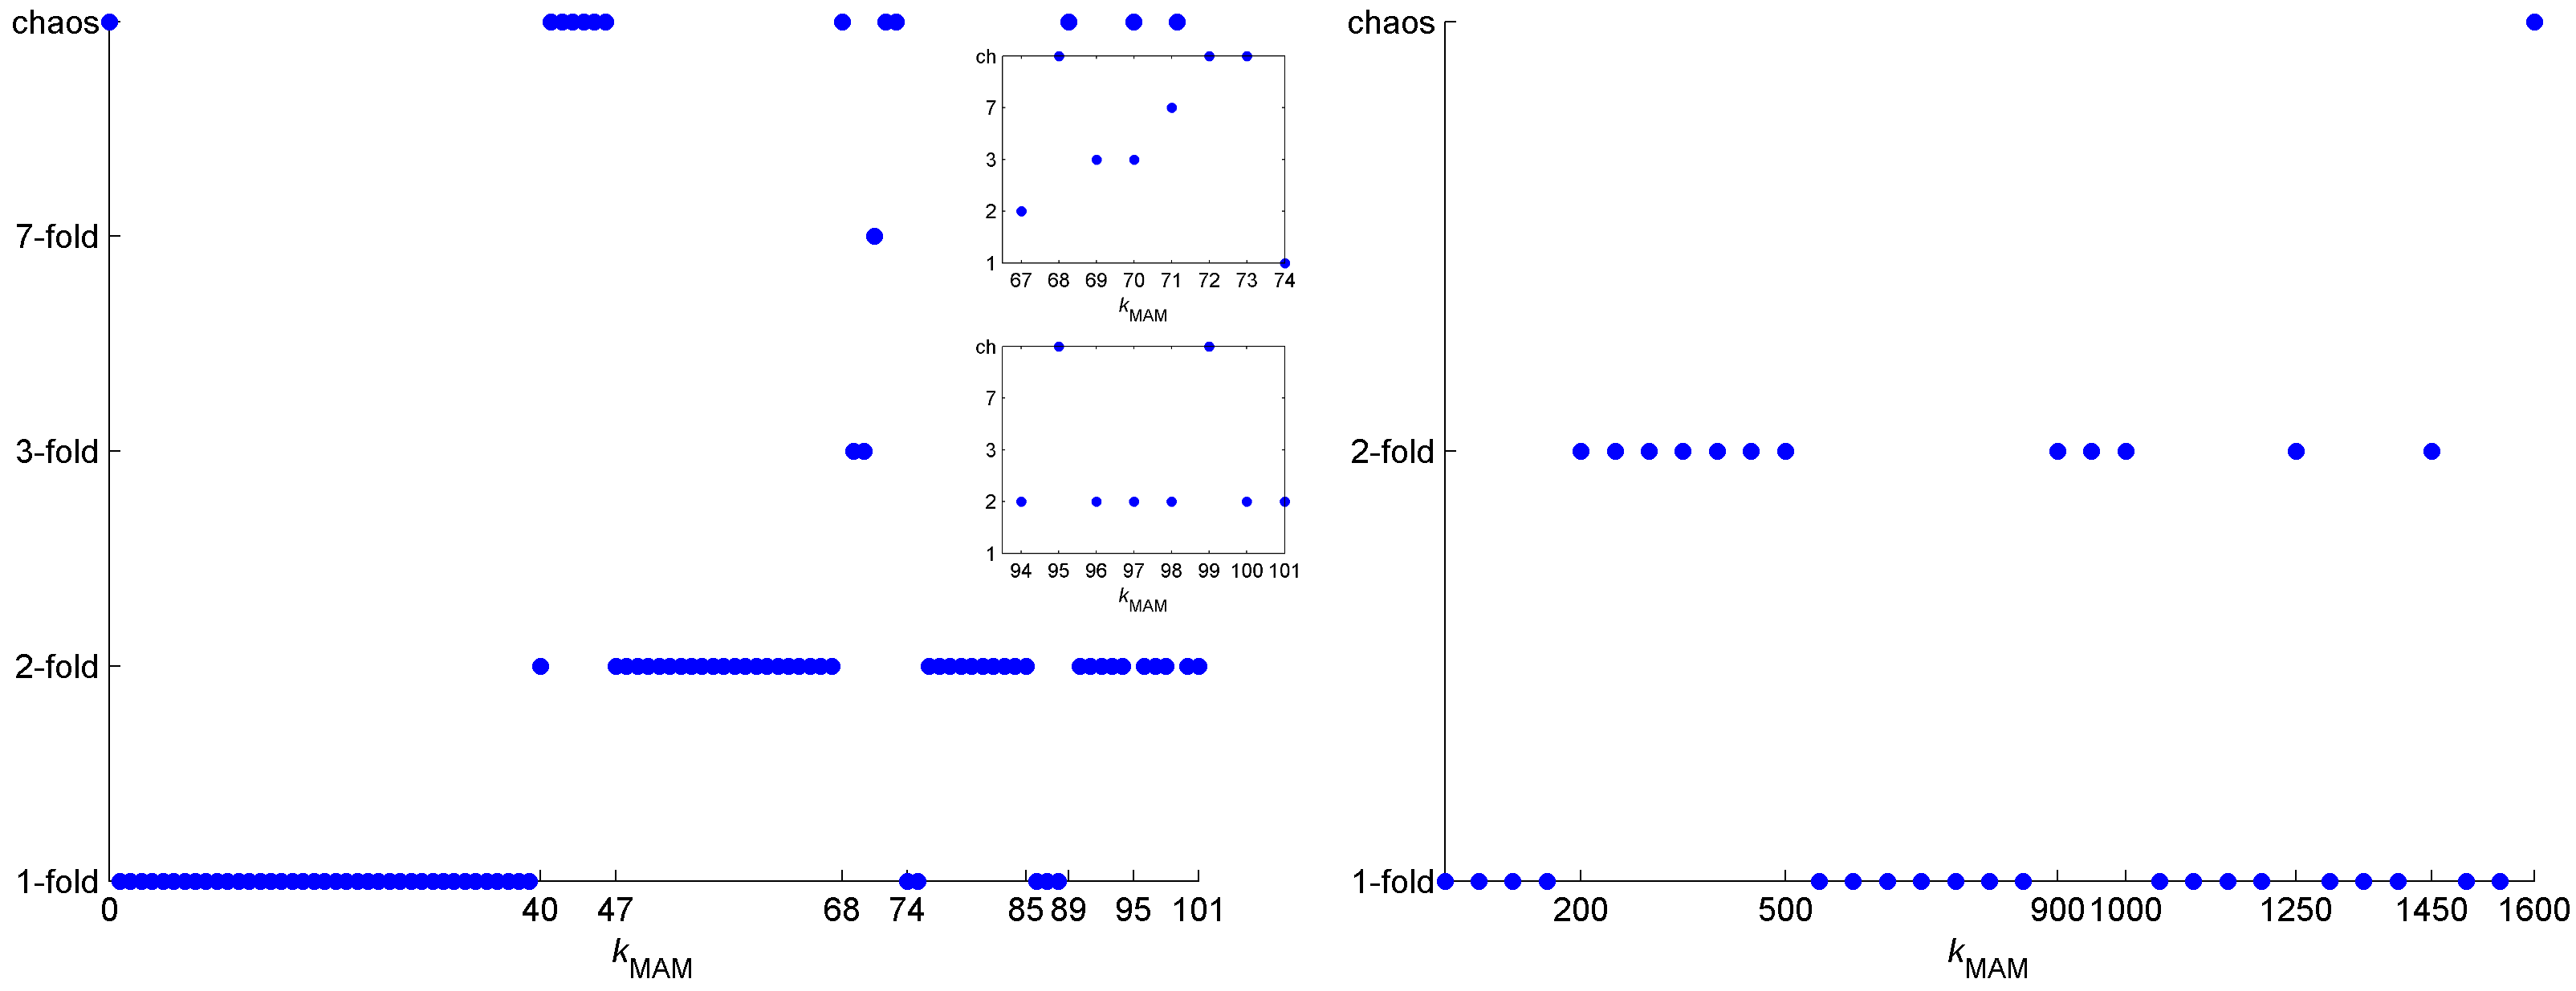
\includegraphics[width=1\textheight]{rysunki/rozdzial_5/jakosciowy}
	\caption[Jakościowa analiza rozwiązań Modelu \#1]{Jakościowy obraz zachowania się rozwiązań przedstawiony w funkcji parametru $k_{MAM}$ dla  $k_{ch}= 2950$ (lewy panel) oraz $k_{ch} = 4100$ (prawy panel). Dla różnych wartości $k_{MAM}$  mamy do czynienia z atraktorem w postaci  1, 2, 3, 7-krotny cyklu granicznego lub trajektorią chaotyczną.}
	\label{fig:jakosciowy}
\end{sidewaysfigure}

Dla parametru $k_{ch}$=4100 dokonaliśmy podobnej analizy zmieniając  parametr $k_{MAM}$ od 0 do 1600 z krokiem równym 50. Stabilne pojedyncze cykle graniczne obecne były dla $k_{MAM}$ z zakresów 0--150, 550--850, 1050--1200, 1300--1400, 1500--1550.  Stabilne podwójne cykle graniczne obecne były dla $k_{MAM}$ z zakresów 200--500, 900--1000 oraz  $k_{MAM}$ równego 1250 i 1450. Zachowania chaotyczne obserwowano dla $k_{MAM}$ równego 1600 (Ryc.~\ref{fig:jakosciowy}, prawy panel). Dla $k_{MAM}\geq 1650$ trajektoria chaotyczna traci stabilność i~większość trajektorii z tego obszaru dąży do punku stacjonarnego, który charakteryzuje się wysokim stężeniem jonów wapnia w przedziale mitochondrialnym. Efekt ten można interpretować jako wczesną fazę procesu apoptozy. Ryc.~\ref{fig:jakosciowy} przedstawia schematycznie uzyskane wyniki dla $k_{MAM}$ z przedziału od 0 -- 1600.

Na Ryc.~\ref{fig:oscylacjeMo1} przedstawiona została mapa zależności okresu oscylacji stężeń jonów wapnia od dwóch parametrów $K_4$ oraz $k_{MAM}$. Okres oscylacji wahał się w przedziale od 11 do 22 sekund. Dla parametru  $K_4 > 3.6$ okres oscylacji praktycznie nie zmieniał się i niezależnie od wartości parametru $k_{MAM}$ wynosił około 12 s. Natomiast dla ustalonej wartości parametru $K_4$ z przedziału (0--3.6) okres oscylacji zwiększał się wraz ze wzrostem wartości parametru $k_{MAM}$

\begin{figure}[ht]
    \centering
    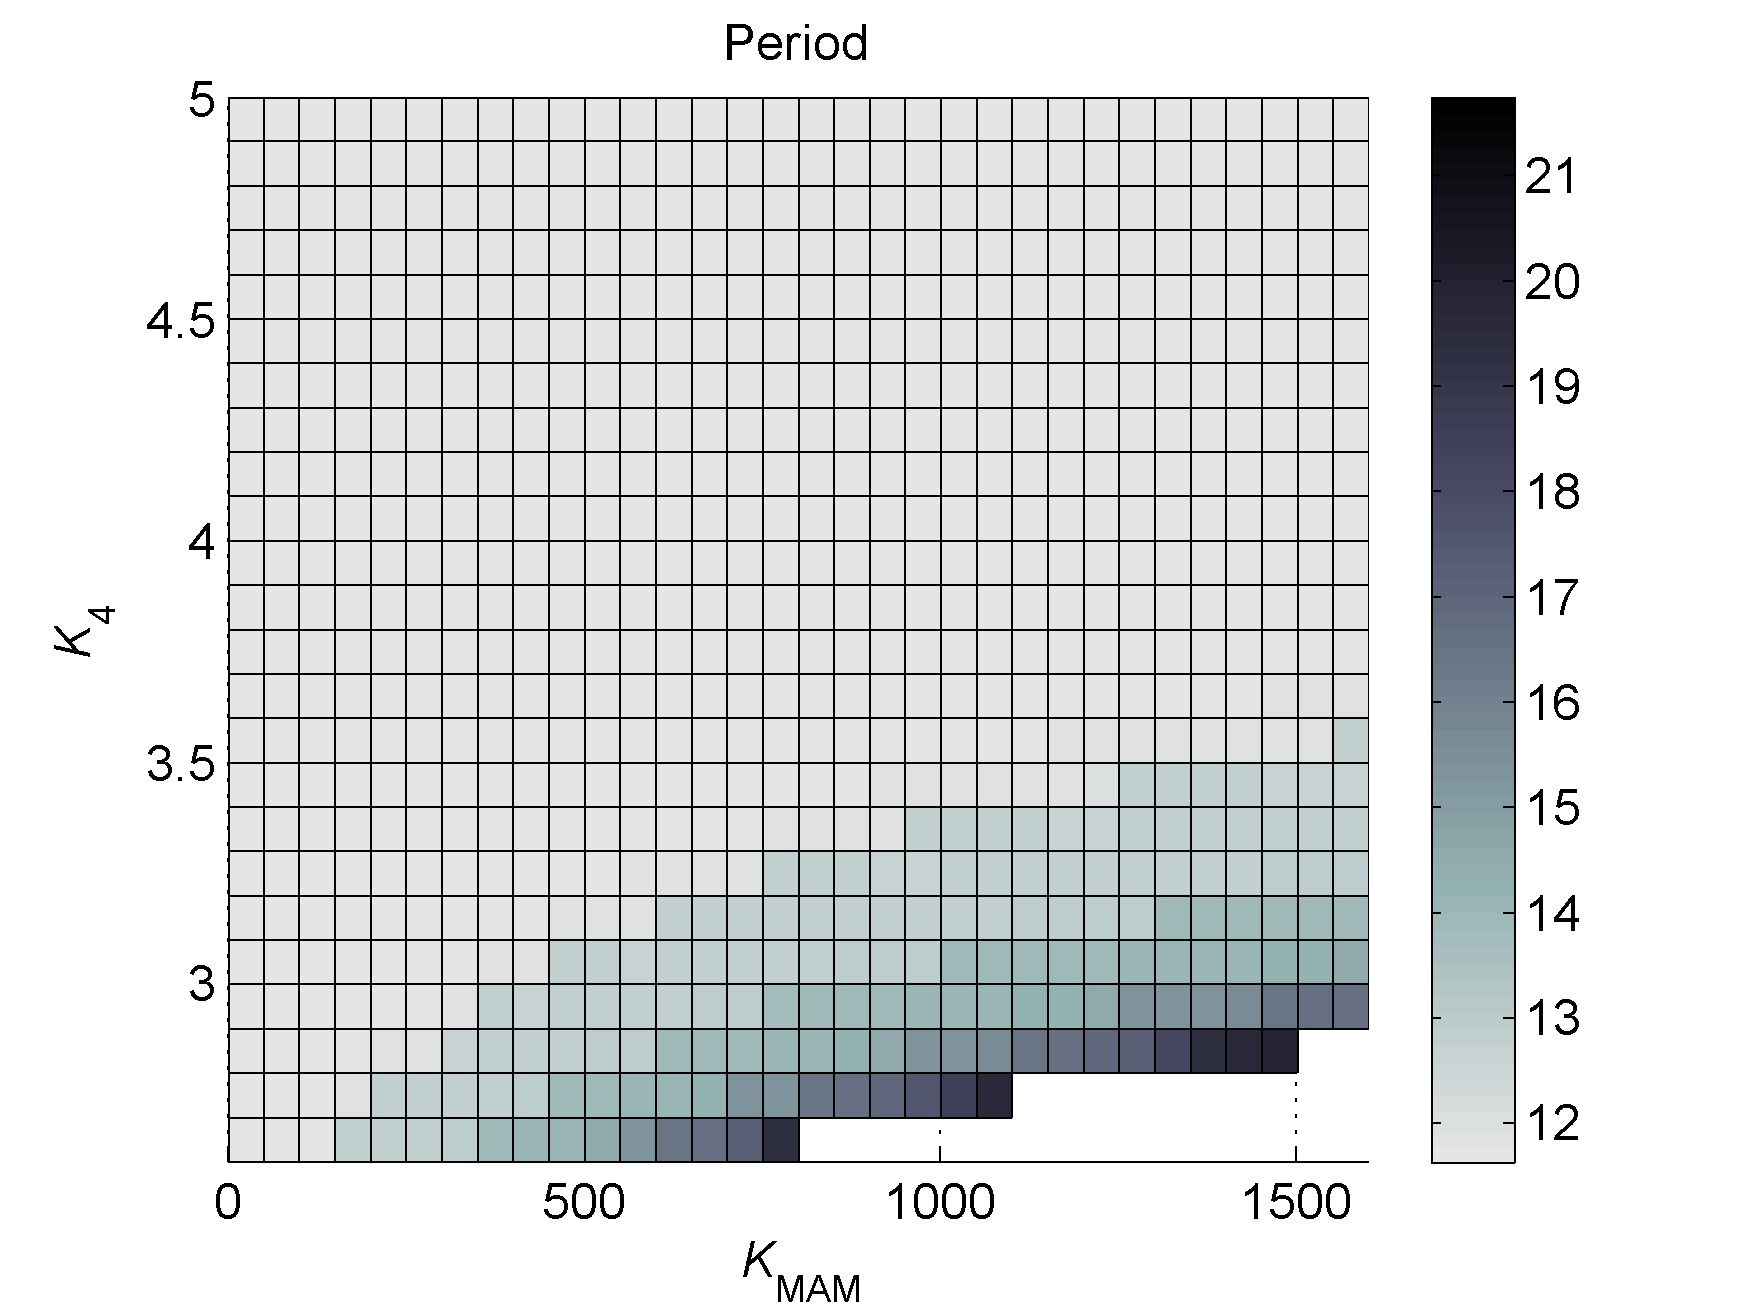
\includegraphics[width=1\textwidth]{rysunki/rozdzial_5/period}
    \caption[Zależność okresu oscylacji od parametrów $k_{MAM}$ i $K_4$]{Zależność okresu oscylacji (w sekundach) od parametrów $k_{MAM}$ i $K_4$ . Biały obszar odpowiada zbiorowi parametrów, dla których rozwiązania periodyczne nie występowały.}
    \label{fig:oscylacjeMo1}
\end{figure}

\FloatBarrier
\subsection{Wpływ $k_{MAM}$ na poziom stężeń jonów wapnia}

Wykresy przedstawiające zmiany minimalnych i maksymalnych wartości stężeń jonów wapnia w Ca$_{Cyt}$ oraz Ca$_{Mit}$ w reżimie stabilnych cykli granicznych, w zależności od współczynnika $k_{MAM}$, znajdują się na Ryc.~\ref{fig:minmaxMo1}. Dla lepszej wizualizacji punkty maksimum i minimum dla wartości $k_{MAM}$ z Ryc.~\ref{fig:jakosciowy} połączone zostały liniami ciągłymi. Minimalne i maksymalne wartości stężeń jonów wapniowych w cytozolu (Ca$_{Cyt}$) pozostają niemal stałe dla obu wartości $k_{ch}$ (2950 i 4100) (prawe panele Ryc.~\ref{fig:minmaxMo1}). Dla $k_{ch} = 2950$ maksymalne Ca$_{Mit}$ charakteryzuje się tendencją wzrostową (pomijając niewielkie perturbacje, wynikające ze zmiany charakteru rozwiązań oscylacyjnych), a~minimalna wartość Ca$_{Mit}$ zmniejsza się. Podobnie dla $k_{ch} = 4100$ obserwujemy istotny wzrost maksymalnych stężeń jonów wapnia w mitochondriach, natomiast minimalne wartości pozostają stabilne nieznacznie maleją. Z tego powodu amplituda oscylacji stężeń jonów wapnia w mitochondrium rośnie wraz z $k_{MAM}$.


\begin{figure}[!ht]
	\centering
	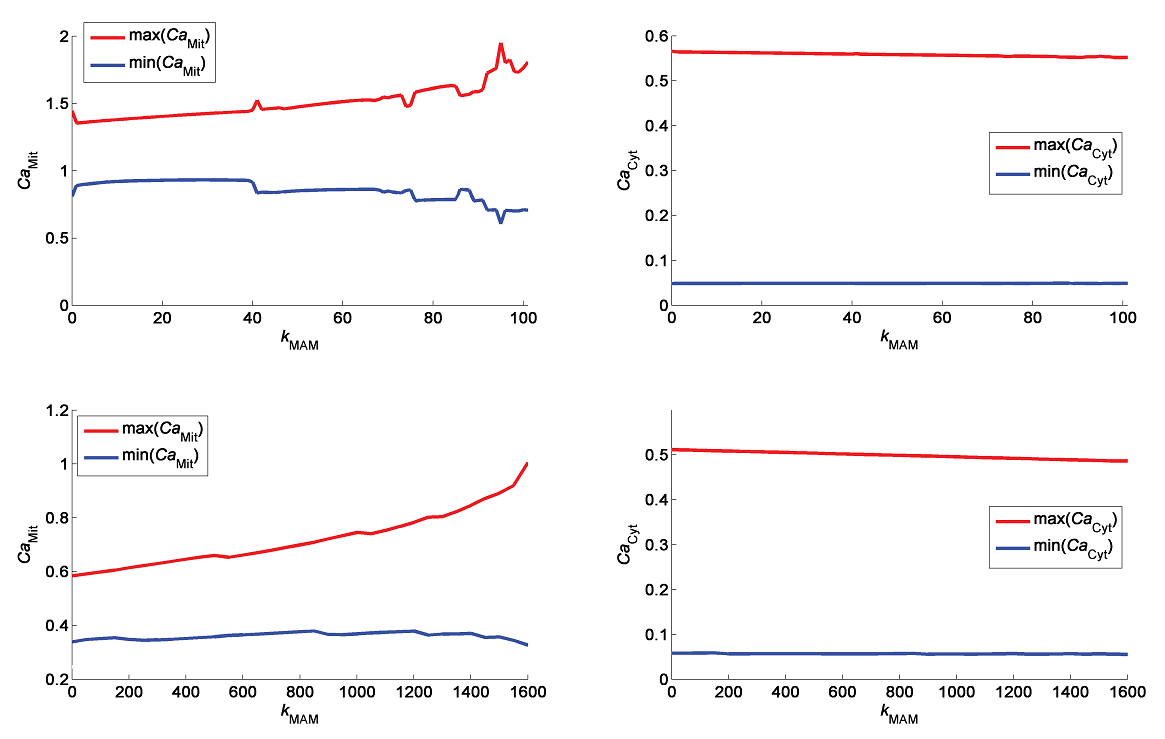
\includegraphics[width=1\textwidth]{rysunki/rozdzial_5/minmaxMo1}
	\caption[Minimalne i maksymalne wartości Ca$_{Mit}$ i Ca$_{Cyt}$]{Minimalne i maksymalne wartości Ca$_{Mit}$ (lewy panel) oraz Ca$_{Cyt}$ (prawy panel) dla rozwiązań periodycznych. Górne panele -  $k_{ch}=2950$, dolne panele - $k_{ch}=4100$. Dla lepszej wizualizacji punkty maksimum i minimum dla wartości $k_{MAM}$ z~Ryc.~\ref{fig:jakosciowy} połączone zostały liniami ciągłymi.}
	\label{fig:minmaxMo1}
\end{figure}




\FloatBarrier
\subsection{Punkty stacjonarne}
\label{ss:steadystatesMo1}

Punkty stacjonarne wyznaczono za pomocą ,,MATLAB - Optimisation Toolbox'', dla zestawu parametrów takich jak przedstawione w Tab.~\ref{tab:constantsMo1}. Na Ryc.~\ref{fig:bifurcationMo1} pokazano zależność stanów stacjonarnych od wartości parametru $k_{MAM}$ w~przedziale 0--10000 (pozostałe parametry tak jak w Tab.~\ref{tab:constantsMo1}). Dla $k_{MAM}=0$ (tak jak ma to miejsce w przypadku modelu Marhla, opisanego w~\cite{Marhl2000}) istnieje tylko jeden dodatni punkt stacjonarny

\[P_{3M} = (Ca_{Cyt} = 0.257, Ca_{ER} = 0.730, Ca_{Mit} = 0.102,  CaPr = 86.41)\]

\noindent (oznaczony na rysunku na niebiesko), który jest niestabilny. Wraz ze wzrostem $k_{MAM}$ zachodzi bifurkacja typu siodło-węzeł już dla wartości $k_{MAM} \approx 0.5$ i pojawiają się dwa nowe stany stacjonarne: stabilny $P_1$ (oznaczony na zielono) oraz niestabilny $P_2$ (oznaczony kolorem czerwonym). Charakterystycznym jest fakt, że dwa pierwsze stany $P_1$ i $P_2$ znacząco zmieniają się wraz ze zmianą wartości $k_{MAM}$, podczas gdy koordynaty punktu $P_3$ prawie wcale się nie zmieniają. Przykładowe punkty stacjonarne dla  $k_{MAM} = 1200$: 

\begin{eqnarray*}
	P_1 &=& (Ca_{Cyt} = 9.18 \times 10^{-3}, Ca_{ER} = 0.892, Ca_{Mit} = 19.1, CaPr = 10.1) \quad \textrm{(stabilny)}\\
	P_2 &=& (Ca_{Cyt} = 0.107, Ca_{ER} = 1.02, Ca_{Mit} = 5.94, CaPr = 62.0) \quad \textrm{(niestabilny)}\\
	P_3 &=& (Ca_{Cyt} = 0.254, Ca_{ER} = 0.730, Ca_{Mit} = 0.173, CaPr = 86.1) \quad \textrm{(niestabilny)}
\end{eqnarray*}



\begin{figure}[ht]
	\centering
	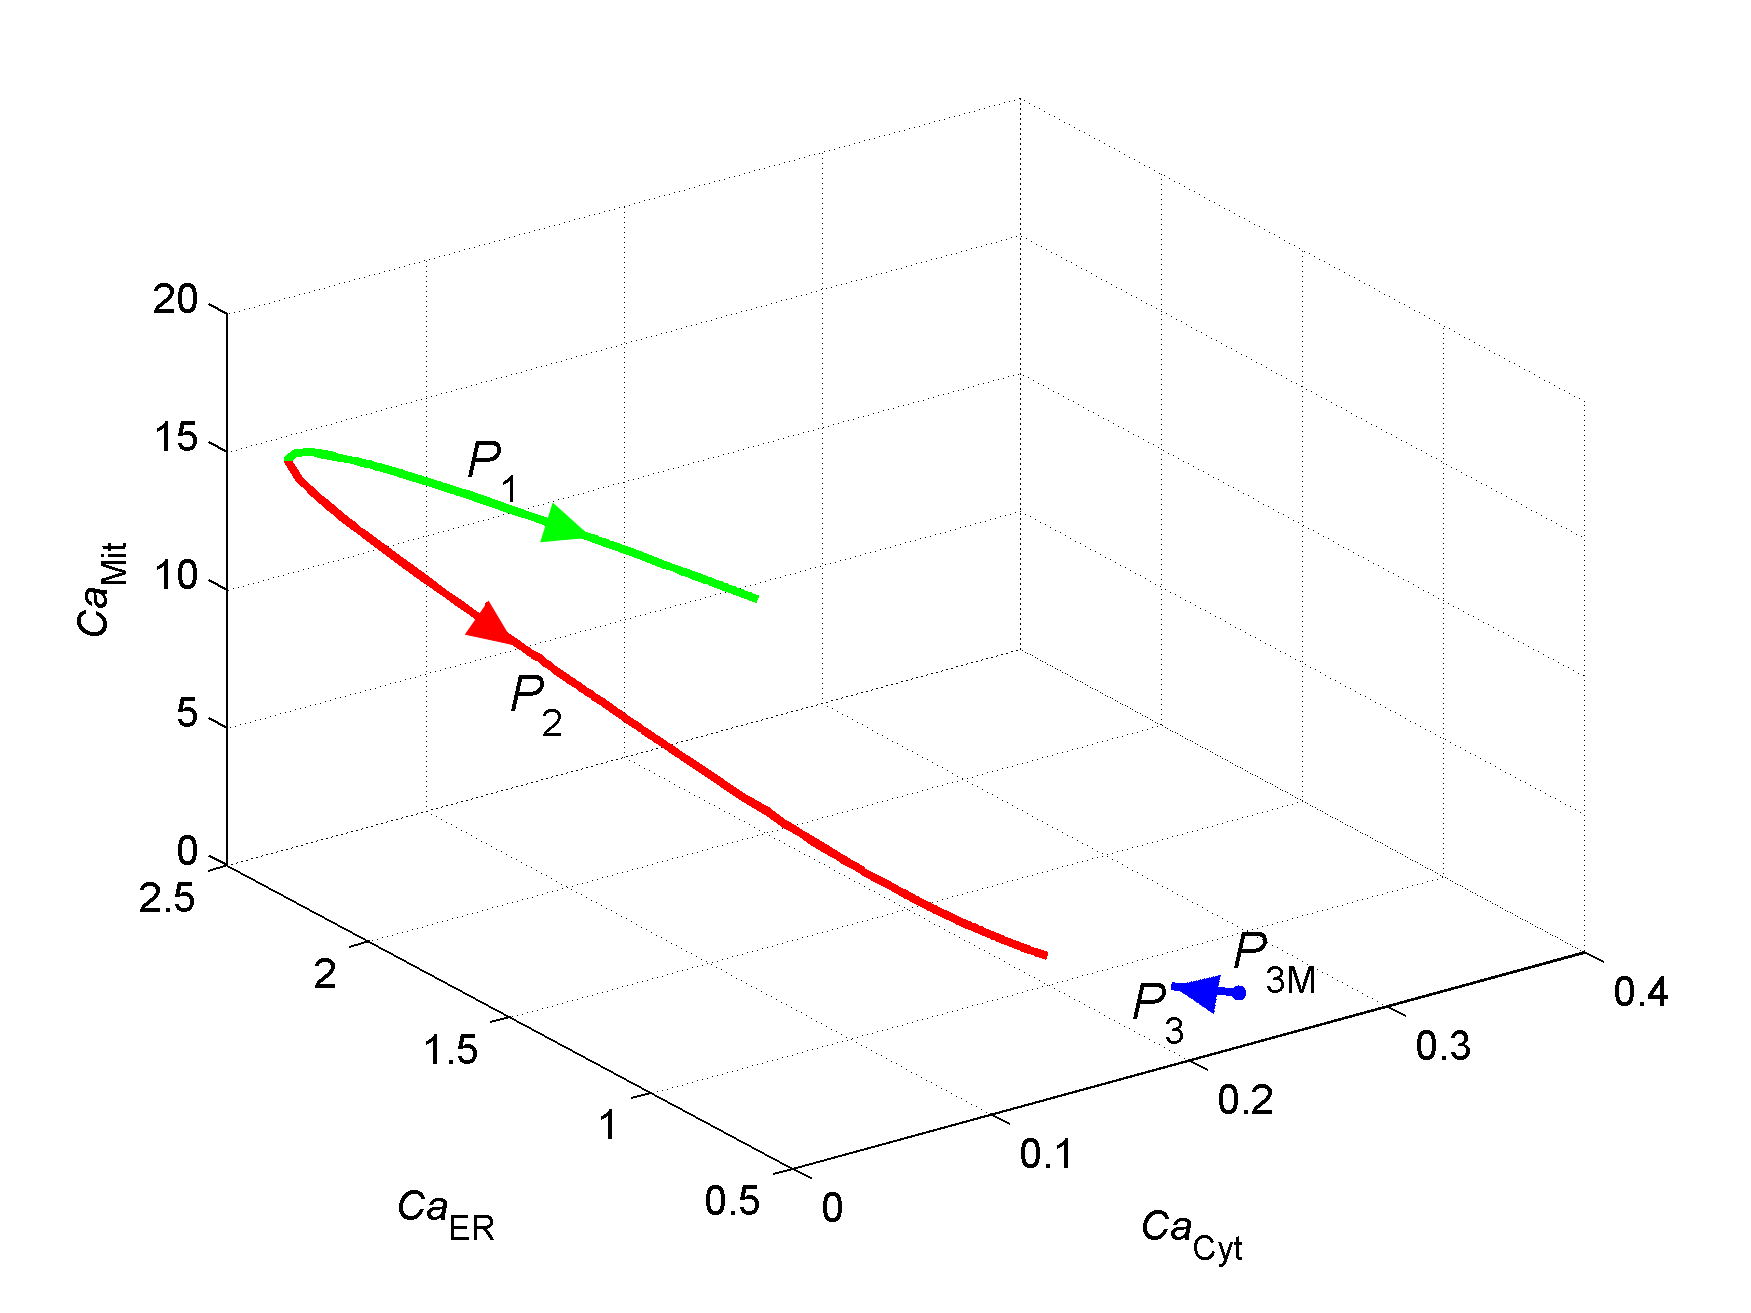
\includegraphics[width=1\textwidth]{rysunki/rozdzial_5/bifurcation}
	\caption[Zachowanie punktów stacjonarnych w Modelu \#1]{Zachowanie punktów stacjonarnych w  $k_{MAM} \in [0, 10000]$: $P_1$ - zielony (stabilny), $P_2$ - czerwony (niestabilny) oraz $P_3$ - niebieski (niestabilny). $P_1$ i $P_2$ powstają w wyniku bifurkacji typu siodło-węzeł przy $k_{MAM}=0.5$. Strzałki wskazują wzrost wartości parametru $k_{MAM}$.}
	\label{fig:bifurcationMo1}
\end{figure}

Ze względu na orientację Ryc.~\ref{fig:bifurcationMo1} nie oddaje dobrze wartości stężeń jonów wapnia w stanach stacjonarnych, w szczególności w kompartmencie mitochondrialnym.
Punkty te wraz z niektórymi trajektoriami do nich dążącymi oraz oraz stabilnym cyklem granicznym  pokazane zostały na Ryc.~\ref{fig:steadystatesMo1}. Jak widać na wykresie istnieje separatrysa łącząca punkty $P_1$ i $P_2$. 

Dla szerokiego zakresu wartości parametru $k_{MAM}$ (np. $k_{MAM} \in (0.5, 1649]$) system zachowuje się jak układ bistabilny, w którym współistnieją dwa atraktory: stabilny punkt stacjonarny $P_1$ oraz stabilny cykl graniczny/przyciągająca trajektoria chaotyczna. jednoczesne istnienie powyższych atraktorów, charakteryzujących się dużymi basenami przyciągania ma istotne znaczenie biologiczne. Oscylacje wapniowe stanowią istotny czynnik będący częścią sieci sygnałowej, sprawdzający czy komórka jest w dobrej kondycji. Natomiast podwyższony napływ jonów wapnia do mitochondriów (realizujący się na trajektoriach przyciąganych do punktu $P_1$) i ich sekwestracja w tym kompartmencie może skierować komórkę na szlak programowanej śmierci (scenariusz apoptozy Rozdz.~\ref{s:scenariusz}). Na Ryc.~\ref{fig:basinofattractionMo1} przedstawiono rzut basenu przyciągania punktu $P_1$ dla parametrów przedstawionych w Tab.~\ref{tab:constantsMo1} na płaszczyzny Ca$_{Cyt}$-Ca$_{ER}$, Ca$_{Cyt}$-Ca$_{Mit}$ i Ca$_{ER}$-Ca$_{Mit}$. Jak widać większość trajektorii układu przyciągana jest przez stabilny cykl graniczny, co oznacza, że oscylacje są odporne na zaburzenia (układ homeostatyczny). Jednakże dla dużych wartości $k_{MAM}$ (np. $k_{MAM} \geq 1649$) to punkt $P_1$ przyciąga znakomita większość trajektorii. Takie zachowanie może być zinterpretowana jako akumulacja wapnia w mitochondriach (pęcznienie mitochondriów), który występują w początkowej fazie apoptozy (podrozdział \ref{s:scenariusz}).


\begin{figure}[ht!]
	\centering
	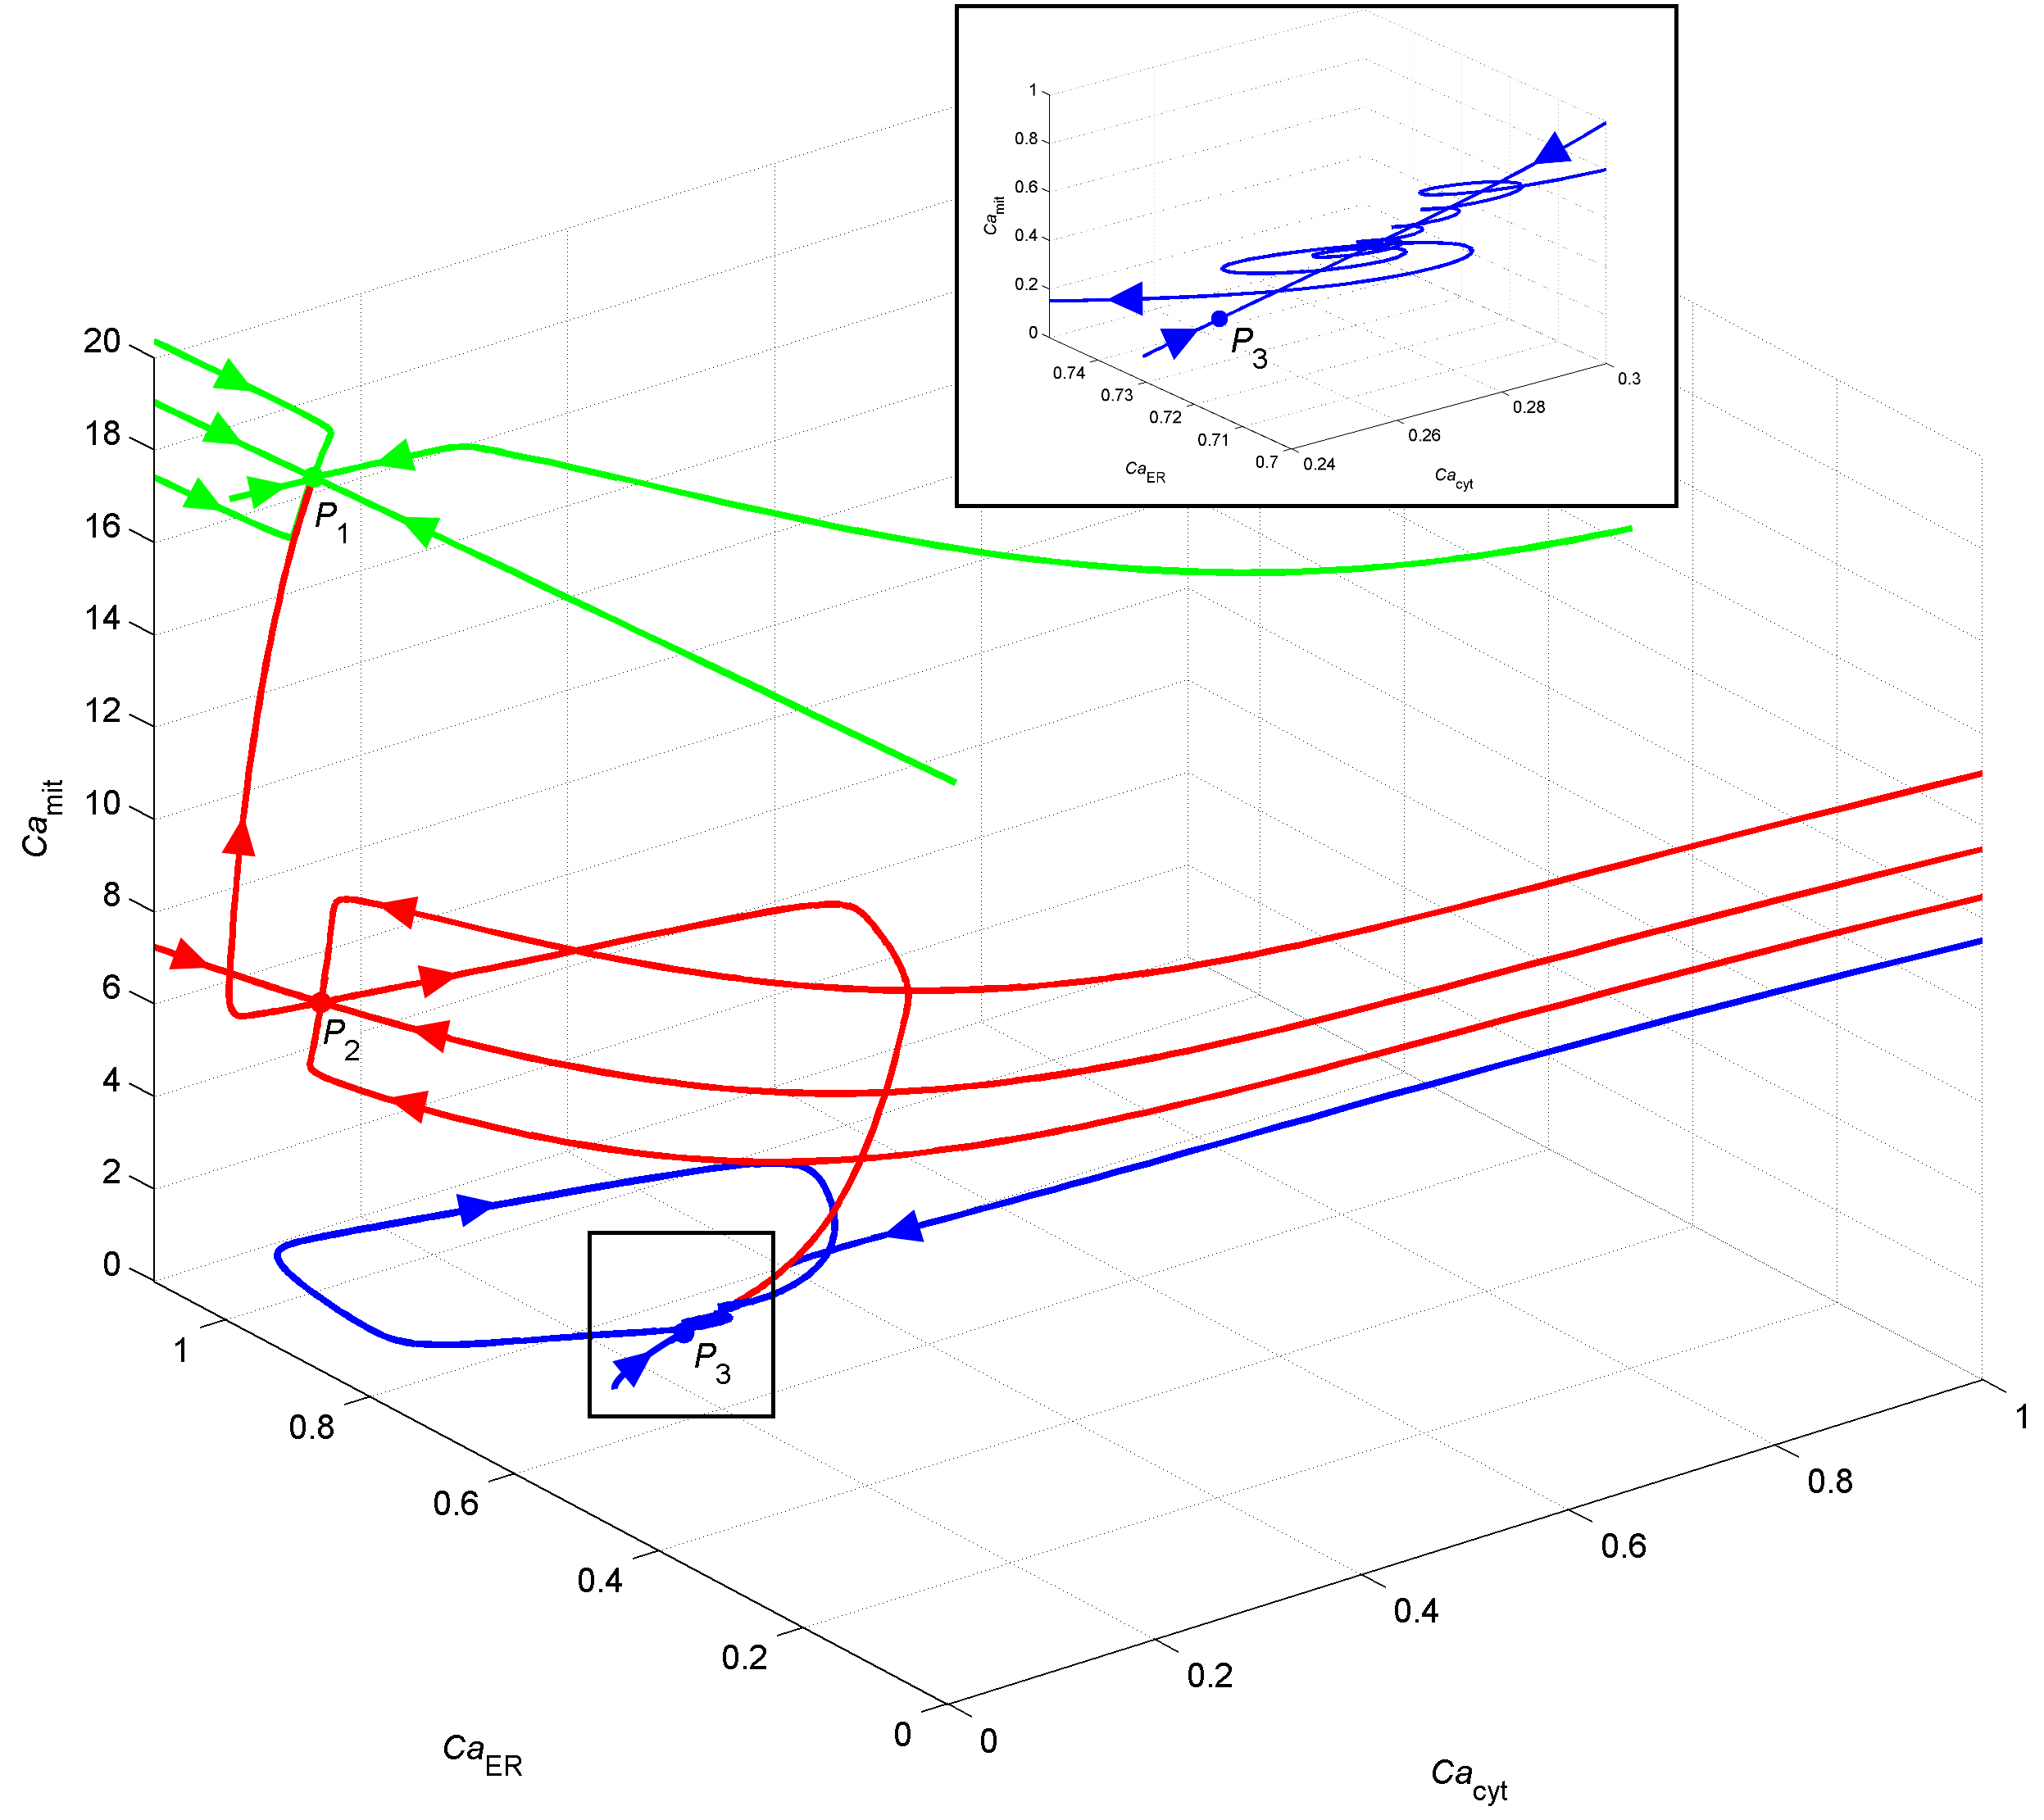
\includegraphics[width=1\textwidth]{rysunki/rozdzial_5/steadystatesMo1}
	\caption[Punkty stacjonarne systemu w Modelu \#1]{Stany stacjonarne $P_1$, $P_2$, $P_3$ systemu (\ref{eq:1}) - (\ref{eq:3}) i stabilny cykl graniczny dla parametrów przedstawionych w Tab.~\ref{tab:constantsMo1}. Punkt $P_3$ pozostaje schowany pod wykresem cyklu granicznego. W powiększeniu widoczny jest złożony charakter oscylacji w pobliżu punktu $P_3$. Kolorami oznaczone są trajektorie przyciągane przez punkty $P_1$, $P_2$, $P_3$.}
	\label{fig:steadystatesMo1}
\end{figure}

\begin{figure}[ht]
	\centering
	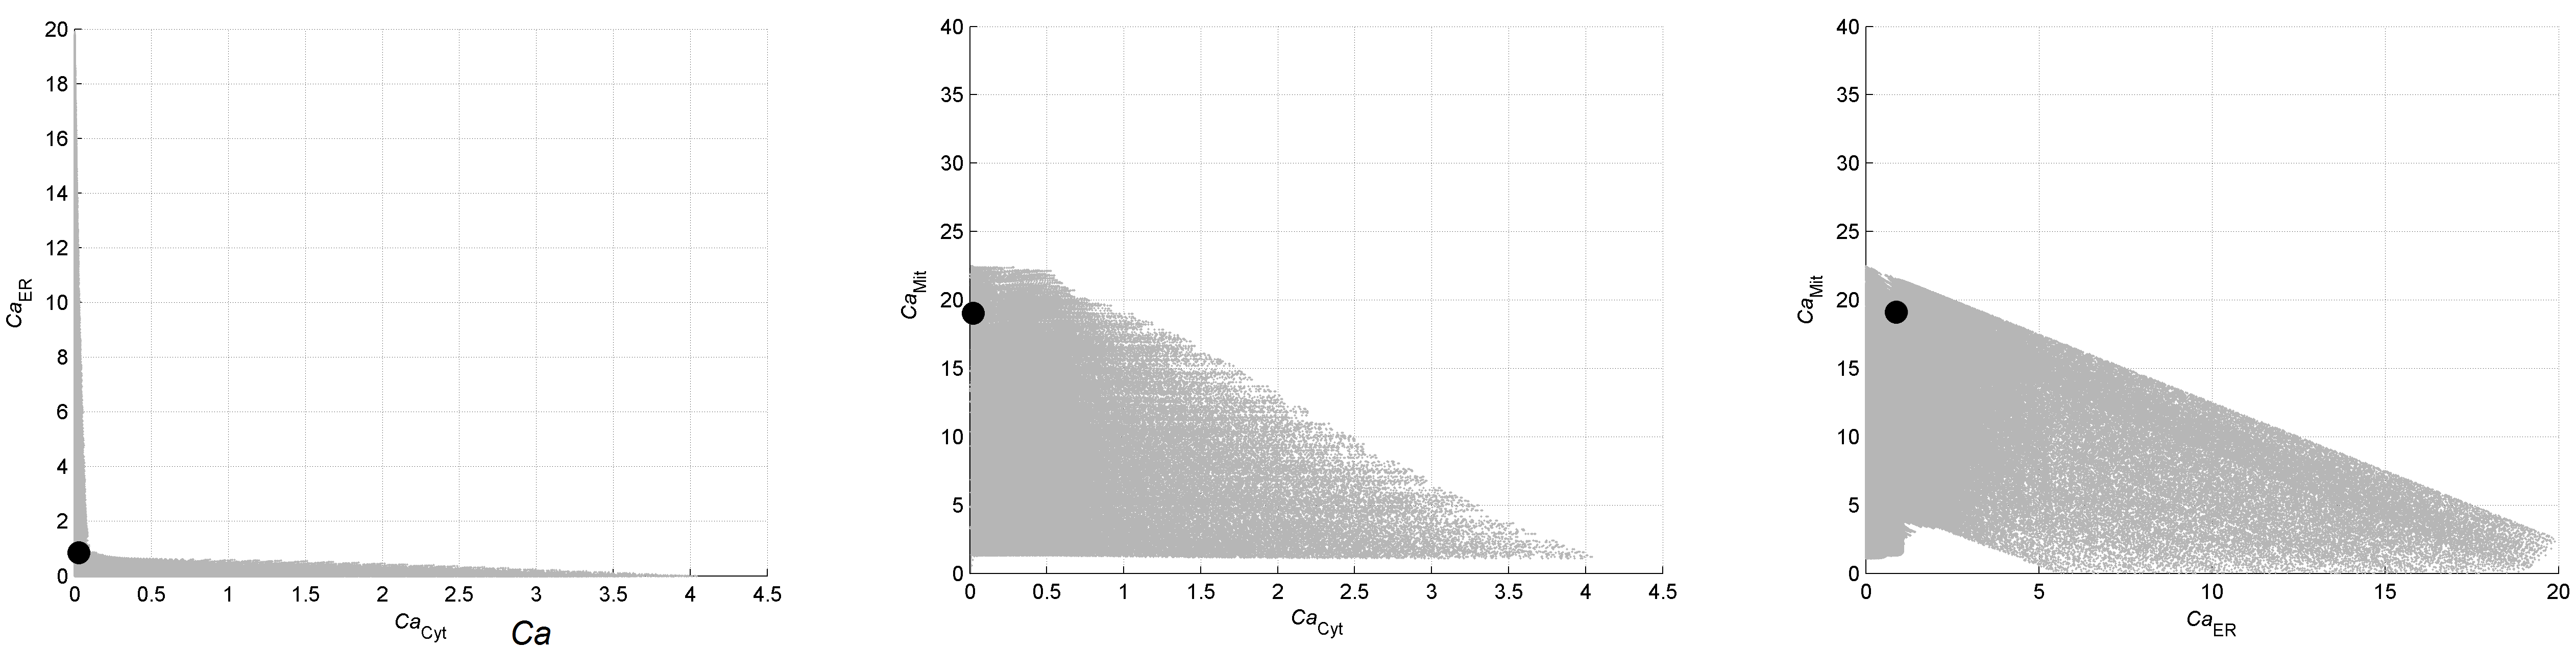
\includegraphics[width=0.85\textwidth]{rysunki/rozdzial_5/basenMo1}
	\caption[Baseny przyciągania punktu $P_1$ w Modelu \#1]{Baseny przyciągania punktu $P_1$: rzutowanie na przestrzeń $Ca_{Cyt} - Ca_{ER}$, $Ca_{Cyt} - Ca_{Mit}$ oraz $Ca_{ER} - Ca_{Mit}$. Czarny punkt odpowiada stabilnemu punktowi stacjonarnemu $P_1 = (9.18 \times 10^{-3}, 0.892, 19.1)$, szare punkty odpowiadają wartościom punktów początkowych trajektorii przyciąganych przez punkt $P_1$. Trajektorie startujące z białego obszaru przyciągane są przez stabilny cykl graniczny.}
	\label{fig:basinofattractionMo1}
\end{figure}



\FloatBarrier
\subsection{Podsumowanie dotyczące Modelu \#1}

Zaproponowany przez nas model (oznaczony jako Model \#1) oscylacji stężeń jonów wapnia (Rozdz.~\ref{ss:Mo1}) uwzględnia jawnie miejsca bliskiego kontaktu mitochondriów i~ER - tzw. struktury MAM. Badania numeryczne wykazały, że   powyższe struktury mają istotny wpływ na rodzaj i kształt profili przebiegów czasowych oscylacji stężeń jonów wapniowych. W modelu tym uzyskano szereg typów oscylacyjnych, od prostych oscylacji stężeń jonów wapnia, przez złożone oscylacje typu ,,bursting'', po quasi-periodyczne rozwiązania chaotyczne. Zmiany parametru $k_{MAM}$ (czyli maksymalnej przepustowości interfejsu MAM) zmienia typ oscylacji. Wzrost $k_{MAM}$ powoduje zazwyczaj regularyzację trajektorii. Np. dla parametrów $k_{ch} = 2950$ i $k_{MAM} = 0$ istnieją rozwiązania chaotyczne, natomiast nawet dla bardzo małych wartości $k_{MAM}$, trajektorie startujące z tych samych warunków początkowych tworzą stabilny cykl graniczny (Ryc.~\ref{fig:jakosciowy}). Wpływ bezpośredniego przepływu wolnych jonów wapnia przez interfejs MAM  nie ogranicza się jedynie do regularyzacji trajektorii. Wraz ze wzrostem przepływu jonów wapnia przez miejsca kontaktu widoczne są bardziej złożone wzorce oscylacji  - reprezentowane przez proste, złożone cykle graniczne i quasi-periodyczne rozwiązania chaotyczne. Ponadto, dla dużych wartości $k_{MAM}$ basen przyciągania rozwiązań oscylacyjnych zmniejsza się znacząco i większość trajektorii zbiega do stabilnego punktu stacjonarnego $P_1$ (Ryc.~\ref{fig:basinofattractionMo1}, charakteryzującego się wysokim poziomem stężenia jonów wapnia w~mitochondriach. Np. dla $k_{MAM} = 1200$ stężenie jonów wapnia w~mitochondriach w punkcie stacjonarnym $P_1$ wynosi $Ca_{Mit} = 19.1 \mu$M. Z biologicznego punktu widzenia tego typu sytuacja może być interpretowana jako początkowa faza procesu apoptozy (tzw. ,,puchnięcie mitochondriów''). Zaobserwowaliśmy również, że wzrost współczynnika $k_{MAM}$ wpływa na kształt profili przebiegów czasowych, tak że dla wysokich wartości $k_{MAM}$ ładowanie mitochondriów wapniem zaczyna się o wiele szybciej, niż w przypadku niskich wartości $k_{MAM}$. Ponadto, amplituda i okres oscylacji oraz średnie stężenie jonów wapnia w~mitochondriach ($Ca_{Mit}$) rośnie z wielkością parametru $k_{MAM}$. Zaproponowany powyżej początkowy etap scenariusza apoptozy jest ściśle związany z~kompleksami błonowymi MAM.


\FloatBarrier
\section{Analiza Modelu \#2}
\label{AnMo2}

Jak już wspomnieliśmy w Rozdz.~\ref{ss:roznice}, w Modelu~\#2  uwzględniono również specyficzne właściwości białka transportującego wapń do wnętrza mitochondrium – uniportera mitochondrialnego (MICU). Białko to przy stosunkowo niskich stężeniach Ca$^{2+}$ przenosi jony wapnia w tzw. szybkim modzie RaM-owym, który jest bardziej efektywny niż mod standardowy. Przepływ wapnia do mitochondriów w tym modelu składa się zatem z~dwóch składowych: pierwsza uwzględnia wspomniany powyżej szybki tryb RaM-owy, druga opisuje pracę uniportera mitochondrialnego w trybie standardowym. Z tego powodu wyrażenia opisujące strumień jonów wapnia wpływających do mitochondriów w obszarze struktur MAM ($J_{MAM})$ i poza nimi ($J_{in}$) składają się z dwóch części, odpowiadających powyższym modom pracy uniportera. Zatem

\begin{align*}
	J_{MAM} &= J_{MAM2} + J_{MAM8} := k_{MAM2} \frac{Ca_{ER}^2}{K_{4,2}^2 + Ca_{ER}^2}% \\[3ex]
	+ k_{MAM8} \frac{Ca_{ER}^8}{K_{4,8}^8 + Ca_{ER}^8},\\
J_{in} &= J_{in2} + J_{in8}:=k_{in2}\frac{Ca_{Cyt}^2}{K_{2,2}^2+Ca_{Cyt}^2} 
				+ k_{in8}\frac{Ca_{Cyt}^8}{K_{2,8}^8+Ca_{Cyt}^8}.
\end{align*}

\noindent gdzie $J_{MAM2}$ i $J_{in2}$ opisują mod RaMowy pracy uniportera, natomiast $J_{MAM8}$ i $J_{in8}$ tryb standardowy.


%W Modelu  \#2 w zależności od wybranych parametrów pojawiają się różne rozwiązania oscylacyjne, oprócz oscylacji chaotycznych, które w tym modelu nie występują. Podobnie również jak w poprzednim modelu stabilne rozwiązania oscylacyjne, odpowiadające stabilnym cyklom granicznym, mają dla większości rozpatrywanych kombinacji parametrów stosunkowo duży basen przyciągania, jednak, wraz ze wzrostem współczynnika $k_{MAM}$, dla prawie wszystkich przypadków trajektorie analizowanego układu są przyciągane przez stabilny punkt stacjonarny układu równań (\ref{eq:1aa})--(\ref{eq:5aa}). Punkt ten charakteryzuje się wysokim stężeniem jonów wapnia w przedziale mitochondrialnym, co jak już wspomniano, z biologicznego punktu widzenia może być utożsamiane z wejściem komórki na ścieżkę apoptotyczną, kiedy to dochodzi do sekwestracji dużych ilości jonów wapnia w mitochondrium i uruchomienia wewnętrznego szlaku apoptozy \cite{Desagher2000,Galluzzi2012,Hajnoczky2006}.

Symulacje numeryczne, których wyniki zostały przedstawione w tym rozdziale w~większości przypadków zostały wykonane dla parametrów przedstawionych w Tab.~\ref{tab:constantsMo2} i~jest to przypadek referencyjny. Jeśli wartości któregoś z parametrów były inne niż w~Tab.~\ref{tab:constantsMo2}, zostało to explicite zaznaczone.

W celu ułatwienia analizy wpływu współczynników $k_{MAM2}$ i $k_{MAM8}$ na zachowanie modelu zdefiniowano dodatkowy parametr $k_{MAM}$:

\begin{equation}\label{suMo2}
k_{MAM} = k_{MAM2} + k_{MAM8}
\end{equation}


\noindent z ustalonym stosunkiem:

\begin{equation}\label{stosunekMo2}
k_{MAM8}/k_{MAM2} = 4
\end{equation}


\noindent W rozdziale tym skoncentrujemy się na:

\begin{itemize}
    \item istnieniu oscylacji stężeń jonów wapnia
    \item stanach stacjonarnych oraz wpływie $k_{MAM}$ na poziom jonów wapniowych
    \item wpływie $k_{MAM}$ na okres oscylacji
    \item możliwym scenariuszu apoptozy wywołanego akumulacją jonów wapnia w mitochondriach
\end{itemize}

Punkty stacjonarne układu (\ref{eq:1aa})--(\ref{eq:5aa}) określone zostały za pomocą programu ,,MATLAB Optimization Toolbox'' dla zestawu parametrów przedstawionych w Tab.~\ref{tab:constantsMo2} i analizowane dalej w odniesieniu do parametru $k_{MAM}$ z użyciem programu MatCont (Matlab Continuation Toolbox) \cite{Dhooge2003}.

\FloatBarrier
\subsection{Analiza przebiegów czasowych}

Przeprowadzone symulacje numeryczne wykazały istnienie   nieregularnych rozwiązań periodycznych dla szerokiego zakresu parametru $k_{MAM}$ (i innych parametrów jak w Tab.~\ref{tab:constantsMo2}). Zauważmy, że ze względu na (\ref{suMo2}) i (\ref{stosunekMo2}) zadając wartość parametr $k_{MAM}$ jesteśmy w stanie wyznaczyć wartości parametrów $k_{MAM2}$ i $k_{MAM8}$. Parametr $k_{MAM}$ w~dalszych rozważaniach będzie parametrem bifurkacyjnym. Jak już wspominaliśmy, w~odróżnieniu od Modelu \#1, w Modelu \#2 nie występują quasi-periodyczne rozwiązania chaotyczne. Wydaje się, że przyczyną tego stanu rzeczy jest inna postać przepływu $J_{out}$ danego przez (\ref{eq:joutMo2}), który w tym przypadku nie zależy od stężenia jonów wapnia w~cytozolu. Oscylacje nieregularne mają dla większości rozpatrywanych zestawów parametrów stosunkowo duży basen przyciągania, jednak, wraz ze wzrostem współczynnika $k_{MAM}$, większość trajektorii układu (\ref{eq:1aa})--(\ref{eq:5aa}) przyciągana jest przez stabilny punkt stacjonarny $P$.

\FloatBarrier
\subsubsection*{Oscylacje stężeń jonów wapnia}

Oscylacje stężeń wolnych jonów wapnia typu ,,bursting'' w poszczególnych kompartmentach oraz czasowy przebieg stężenia uwapniowanych buforów w cytozolu ($CaPr$) zostały przedstawione na Ryc.~\ref{fig:complexoscillationsMo2}. Odpowiadający tym oscylacjom portret fazowy w~przestrzeni $Ca_{Cyt}$, $Ca_{Mit}$, $Ca_{ER}$ pokazany jest na Ryc.~\ref{fig:phaseportraitcomplexMo2}. Parametry, dla których istnieją tego typu rozwiązania oscylacyjne przedstawiono w Tab.~\ref{tab:constantsMo2}. Oscylacje te charakteryzują się powolnym wypływem jonów wapnia z kompartmentu mitochondrialnego oraz szybką wymianą jonów wapnia pomiędzy cytozolem i ER.



\begin{figure}[ht]
	\centering
	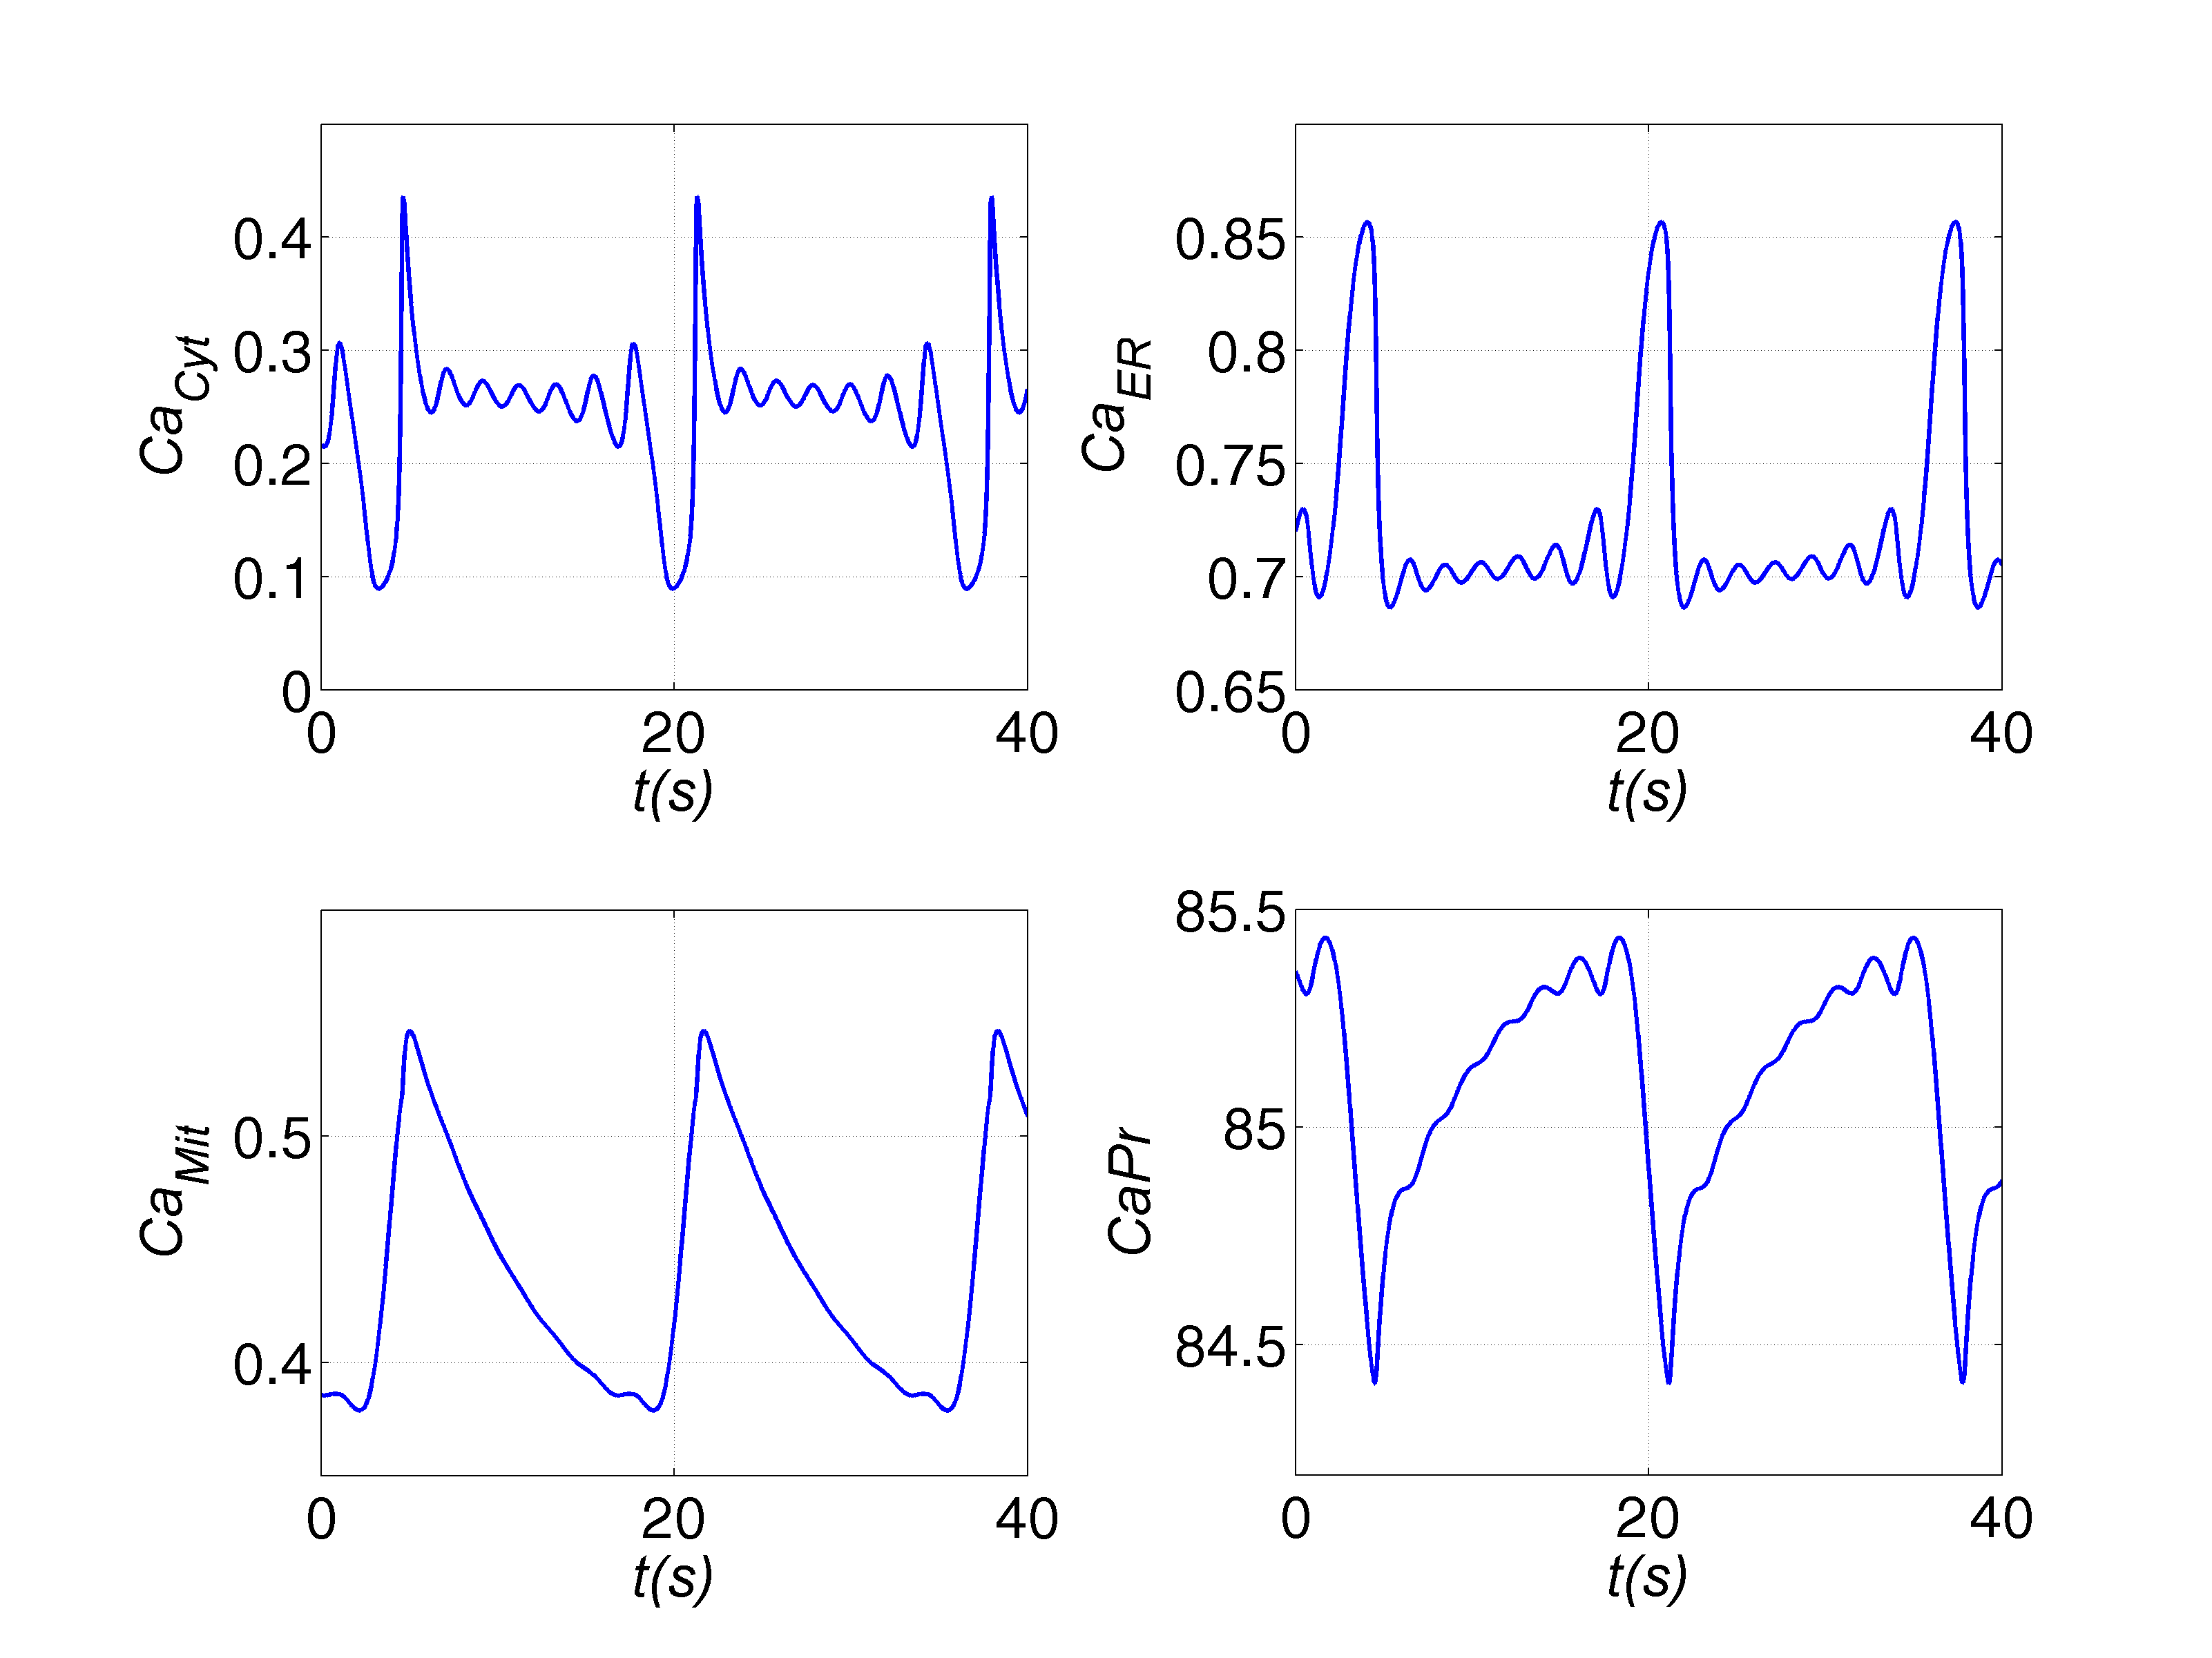
\includegraphics[width=0.95\textwidth]{rysunki/rozdzial_5/bursting_timecourseMo2}
	\caption[Oscylacje wapniowe typu ,,bursting'' w Modelu \#2]{Trajektorie oscylacji wapniowych, zmiany stężenia wapnia w poszczególnych kompartmentach: gwałtowne oscylacje typu ,,bursting''}
	\label{fig:complexoscillationsMo2}
\end{figure}

\begin{figure}[ht]
	\centering
	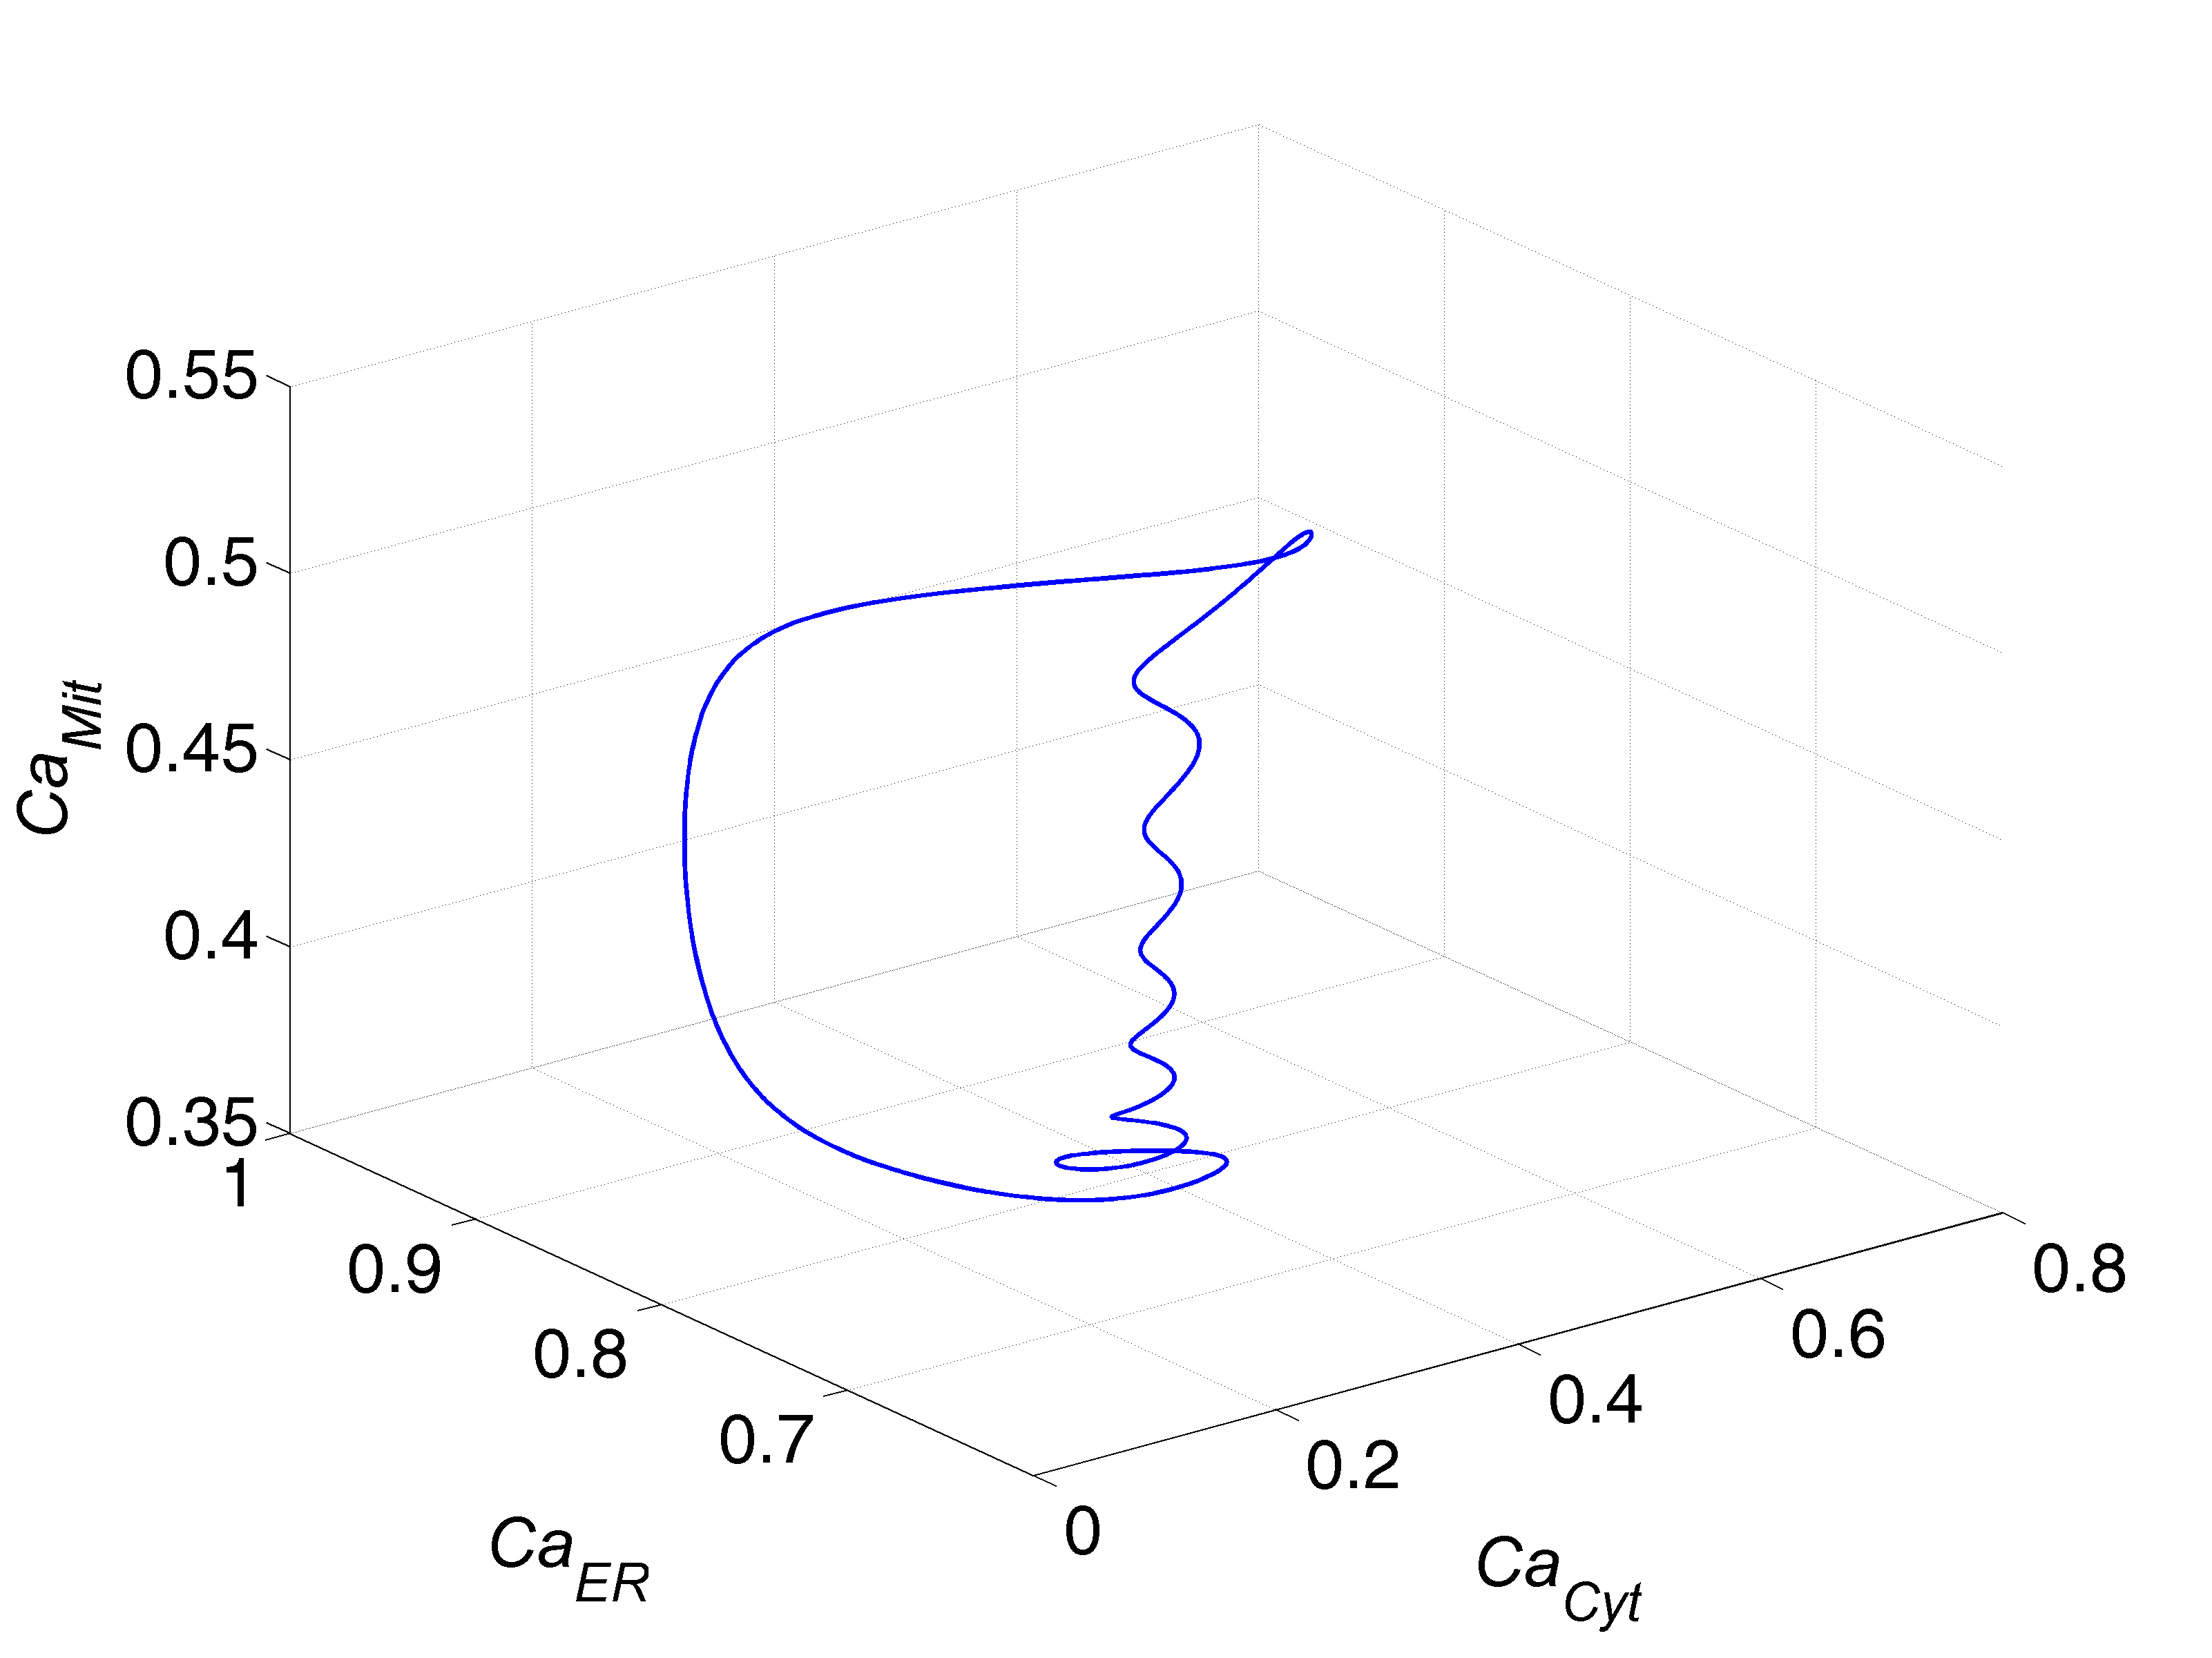
\includegraphics[width=0.95\textwidth]{rysunki/rozdzial_5/bursting_cycleMo2}
	\caption[Portret fazowy 3-D - oscylacje ,,bursting'' w Modelu \#2]{Trójwymiarowy portret fazowy oscylacji typu ,,bursting''. Wszystkie parametry tak jak w Tab.~\ref{tab:constantsMo2}}
	\label{fig:phaseportraitcomplexMo2}
\end{figure}

%\FloatBarrier
%\subsubsection*{Oscylacje regularne}
%
%Na Rycinach \ref{fig:regularoscillationsMo2}~i~\ref{fig:phaseportraitregularMo2} przedstawiono \emph{regularne} oscylacje stężenia jonów wapnia w~poszczególnych  kompartmentach oraz obraz cyklu granicznego w przestrzeni  fazowej $Ca_{Cyt}$, $Ca_{Mit}$, $Ca_{ER}$ dla parametrów jak w Tab.~\ref{tab:constantsMo2}. Oscylacje te maja charakter regularny. Okres oscylacji $T$ wynosi 10.8 s, natomiast stężenia jonów wapnia  w poszczególnych kompartmentach zawierały się w przedziałach: (0.054, 0.65) dla $Ca_{Cyt}$, (0.41, 0.96) dla $Ca_{Mit}$, (0.72, 1.11) dla $Ca_{ER}$, natomiast ilość wapnia zbuforowanego $CaPr$ zawierała się w przedziale (81.9, 85.11). Podobnie jak w przypadku z Modelu \#1 brak jest tutaj komponenty o podwyższonej ,,częstotliwości'', która występuje w~przypadku oscylacji typu ,,bursting'' (Ryc.~\ref{fig:complexoscillationsMo2}).
%
%\begin{figure}[ht]
%	\centering
%	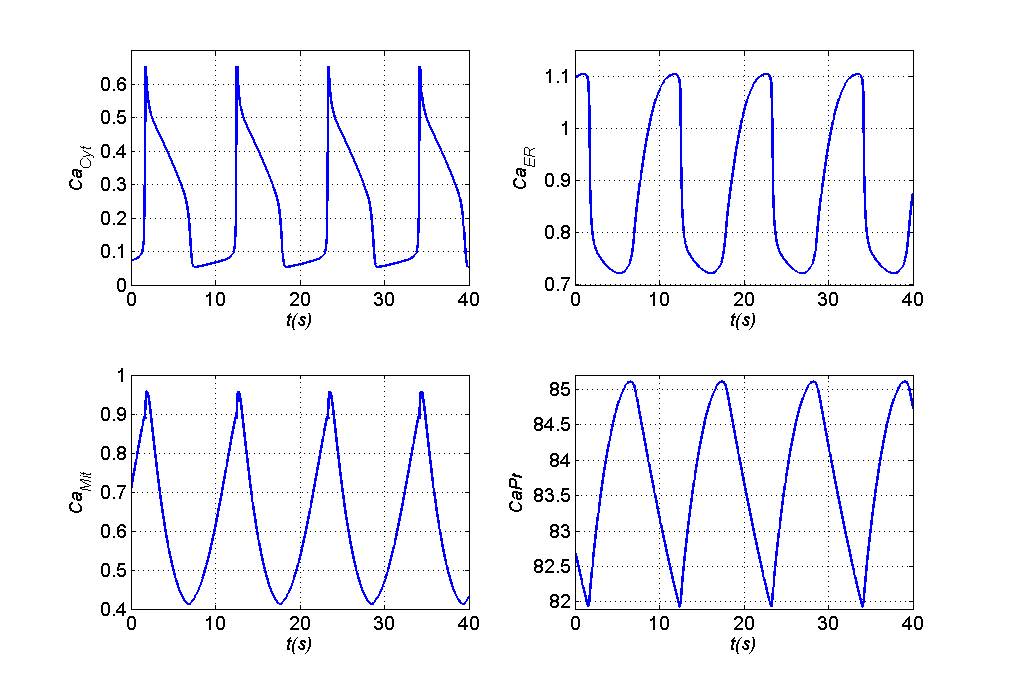
\includegraphics[width=1\textwidth]{rysunki/rozdzial_5/regular_timecourseMo2}
%	\caption[Regularne oscylacje wapniowe w Modelu \#2]{Trajektorie regularnych oscylacji wapniowych, zmiany stężenia wapnia (w~$\mu$M) w~poszczególnych kompartmentach komórki. Parametry przedstawiono w~Tab.~\ref{tab:constantsMo2}.}
%	\label{fig:regularoscillationsMo2}
%\end{figure}
%
%\begin{figure}[ht]
%	\centering
%	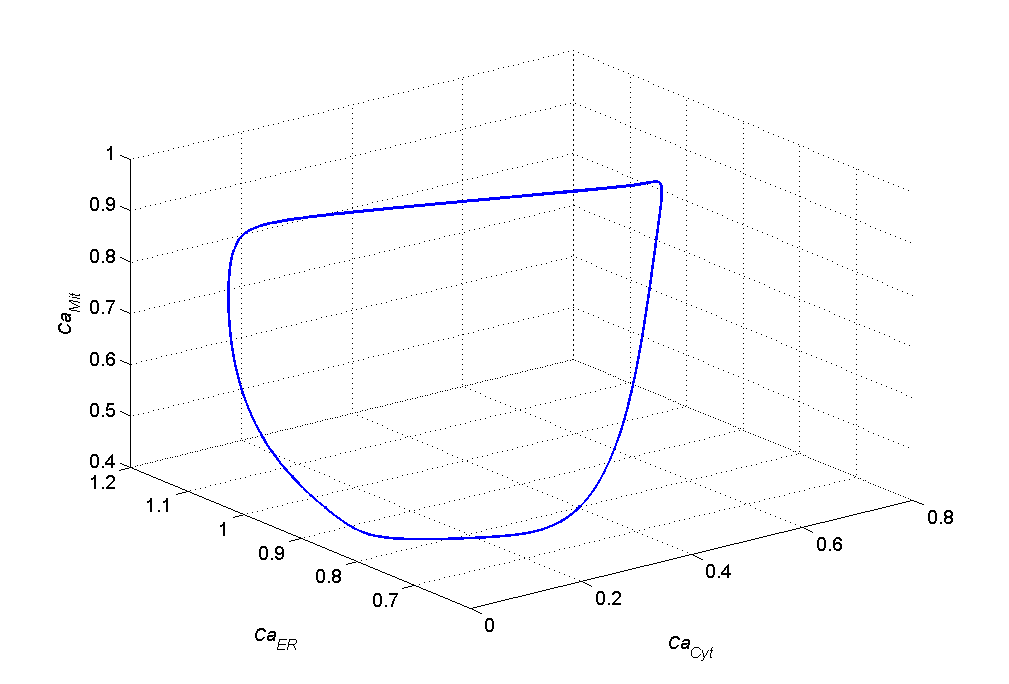
\includegraphics[width=1\textwidth]{rysunki/rozdzial_5/regular_cycleMo2}
%	\caption[Portret fazowy - oscylacje regularne w Modelu \#2]{Trójwymiarowy portret fazowy regularnych oscylacji wapnia dla parametrów jak w~Tab.~\ref{tab:constantsMo2}.}
%	\label{fig:phaseportraitregularMo2}
%\end{figure}

\FloatBarrier
\subsubsection*{Analiza pojedynczego cyklu oscylacji typu ,,bursting''}

Pojedynczy okres oscylacji nieregularnych typu ,,bursting'', dla zestawu parametrów jak w Tab.~\ref{tab:constantsMo2}, przedstawiono na Ryc.~\ref{fig:jedenOkresMo2}. Każdy cykl może być podzielony na trzy fazy. Faza I - zaczyna się, gdy poziom wapnia w cytozolu ($Ca_{Cyt}$) osiąga wartość maksymalną ($t = 4.4$~s) i trwa do czasu aż poziom wapnia w mitochondriach ($Ca_{Mit}$) osiągnie wartość maksymalną ($t = 4.8$ s). W tej fazie wiodącymi procesami są: uwalnianie wolnych jonów wapnia z~retikulum oraz znaczny pobór $Ca^{2+}$ przez mitochondria i buforowanie poprzez białka cytozolu. 

W fazie drugiej aktywowany jest powolny strumień jonów wapnia z~mitochondriów do cytozolu. Większość uwolnionych jonów wapnia związana jest z~cytozolicznymi białkami buforującymi. Ważnym procesem, zachodzącym w tej fazie jest szybka wymiana wapnia pomiędzy cytozolem i ER, co prowadzi do małych, szybkich drgań stężenia wapnia w~tych kompartmentach. Ten etap kończy się, gdy poziom wapnia buforowanego ($CaPr$) osiąga wartość maksymalną (tj. dla $t = 18.1$ s).

W fazie III, wiodącym procesem jest dysocjacja kompleksów białkowo-wapniowych. Mitochondria i ER są "ładowane", podczas gdy poziom wapnia w cytozolu najpierw zmniejsza się, a następnie wzrasta, aby osiągnąć maksymalną wartość, która wyznacza koniec III fazy ($t = 21.05$ s). 

Cały okres trwa 16.65 sekundy, a stężenia wolnych jonów wapnia w poszczególnych kompartmentach wahają się w przedziałach: (0.089, 0.44) dla  $Ca_{Cyt}$, (0.69, 0.86) dla $Ca_{ER}$,  (0.38, 0.55) dla $Ca_{Mit}$ oraz (84.4, 85.4) dla $CaPr$.

\begin{figure}[ht]
    \centering
    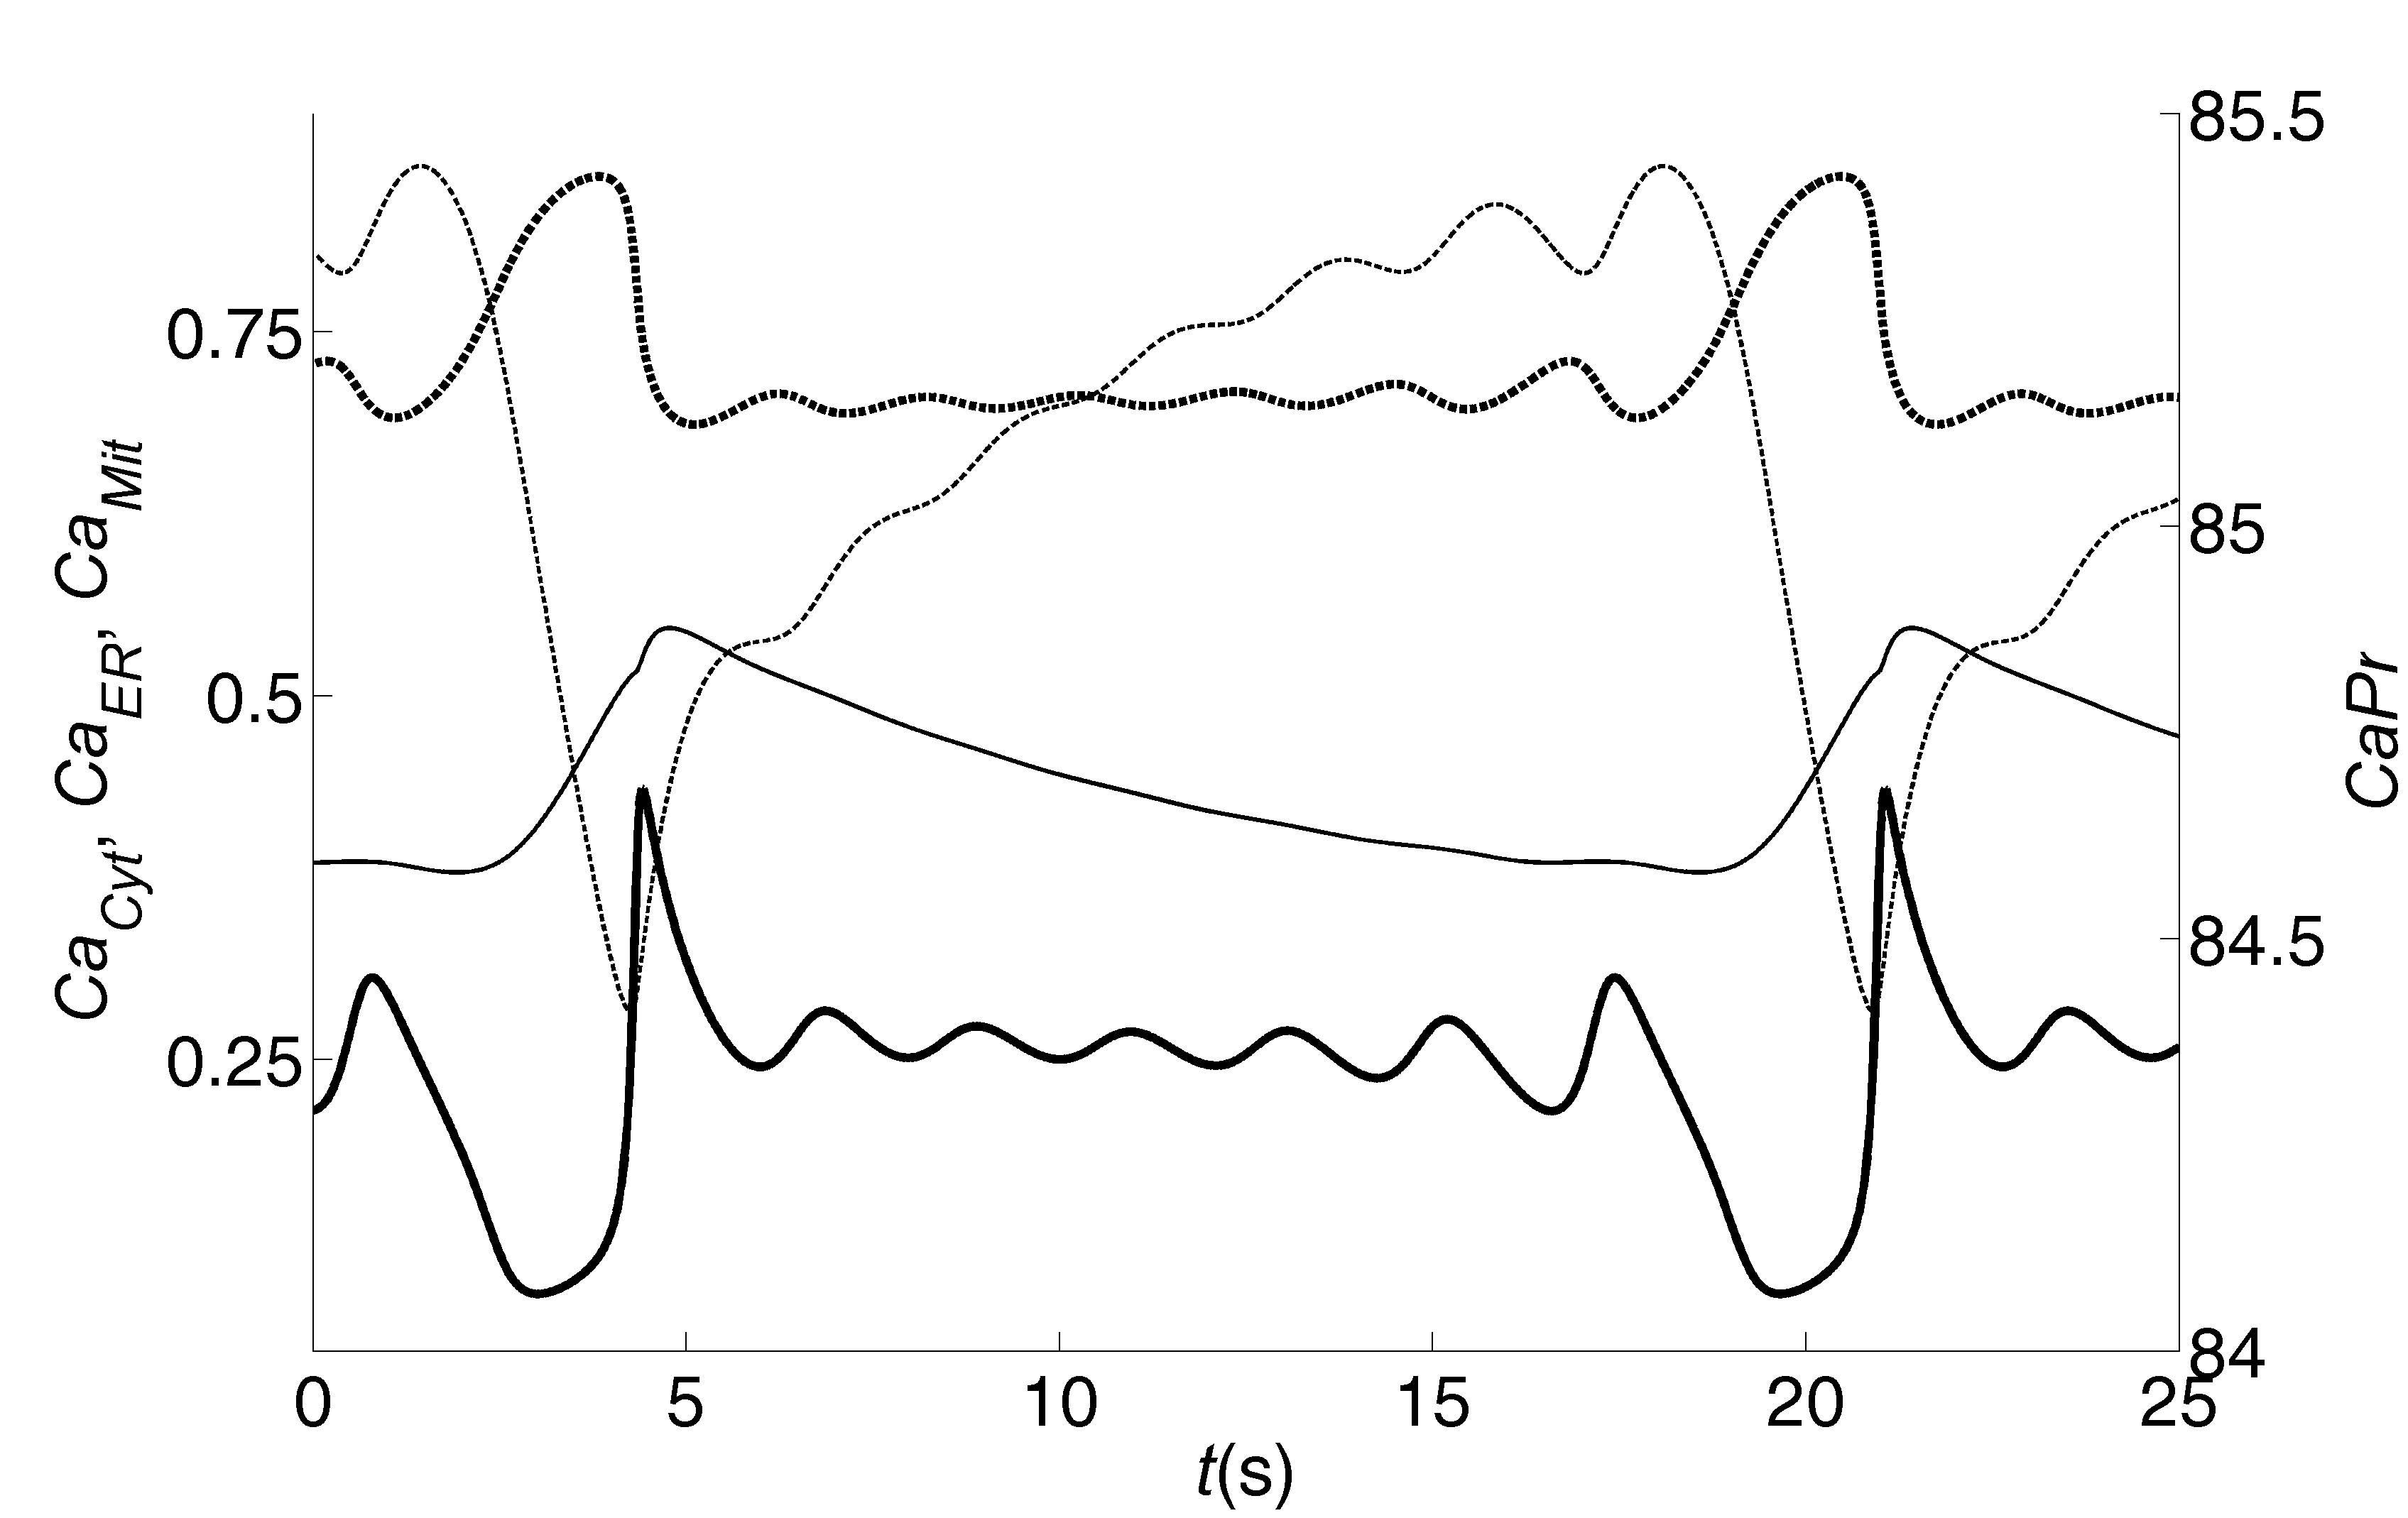
\includegraphics[width=1\textwidth]{rysunki/rozdzial_5/one_periodMo2}
    \caption[Przebiegi czasowe, jeden okres w Modelu \#2]{Przebiegi czasowe  stężeń jonów wapnia w cytozolu, retikulum i mitochondriach dla jednego okresu oscylacji. $Ca_{Cyt}$ - gruba, ciągła linia, $Ca_{Mit}$ - cienka, ciągła linia, $Ca_{ER}$ - gruba, przerywana linia, $CaPr$ - cienka, przerywana linia.}
    \label{fig:jedenOkresMo2}
\end{figure}

Powyższe przebiegi czasowe częściowo przypominają wyniki pomiarów opisanych w~\cite{Ishii2006} po aktywacji histaminą, mimo że w \cite{Ishii2006} autorzy brali pod uwagę oscylacje, które miały tendencje zanikowe, w wyniku czego ustalał się nowy stan równowagi. W eksperymentach przeprowadzonych przez \cite{Ishii2006} pik stężenia wapnia cytozolicznego ($Ca_{Cyt}$) poprzedzał pik stężenia wapnia mitochondrialnego ($Ca_{Mit}$), oraz minimum wapnia retikularnego ($Ca_{Er}$), tak jak w prezentowanym powyżej modelu. Podobne były też minima i maksima przebiegów czasowych stężeń jonów wapnia. Kolejnym podobieństwem pomiędzy pomiarem eksperymentalnym, a~oscylacjami przedstawionymi na Ryc.~\ref{fig:jedenOkresMo2}, jest prosty, liniowy, spadek stężenia jonów wapnia w mitochondriach w odróżnieniu od  oscylacyjnego spadku jonów wapnia w cytozolu (składowa o niskiej amplitudzie i wysokiej częstotliwości widoczna na Ryc.~\ref{fig:jedenOkresMo2} między $t \cong 6$ i $t \cong 18$ sekundą). Dodatkowo profil przebiegów czasowych i poziom stężeń jonów wapnia w~cytozolu na Ryc.~\ref{fig:jedenOkresMo2} podobne są do wykresu danych eksperymentalnych przedstawionego na Ryc.~1 w~pracy \cite{Borghans1997}.

\subsubsection{Przepływy domitochondrialne}
Przepływy przez struktury MAM mogą stanowić istotny czynnik wpływający na dynamikę przedstawionego w tym rozdziale modelu. W celu weryfikacji powyższej hipotezy przeprowadziliśmy porównanie przepływów mitochondrialnych $J_{in}$ i $J_{MAM}$ (Ryc.~\ref{fig:complexoscillationsMo2} - lewy panel).

%Zanalizowano dwa przepływy do mitochondrium, które charakteryzują się różnym pochodzeniem (lewy panel Ryc.~\ref{fig:przeplywy2}): $J_{in}$ (wapń pochodzenia cytozolicznego) oraz $J_{MAM}$ (wapń pochodnia retikularnego).
Pomimo, że przepływ $J_{in}$ charakteryzuje się nieznacznie wyższą wartością maksymalną, to całkowity przepływ jonów wapniowych przez struktury MAM jest większy. Całkowity przepływ przez struktury MAM wynosił \[\int_t^{t+T} J_{MAM}(s) \, ds = 3.55\]
w trakcie jednego okresu równego $T = 16.65$~s i przewyższał przepływ przez uniportery usytuowane poza MAM 
\[\int_t^{t+T} J_{in}(s) \, ds = 0.37\].
Prawy panel pokazuje dwie składowe wpływu wapnia do mitochondrium wewnątrz struktur MAM, które odpowiadają dwóm modułom pracy uniportera: trybowi normalnemu - $J_{MAM2}$ oraz trybowai RaM  - $J_{MAM8}$, które zdefiniowane zostały w równaniu (\ref{eq:jmamMo2}). Maksymalne wartości przepływu $J_{MAM2}$ są mniejsze od maksymalnych wartości przepływu $J_{MAM8}$, a całkowity przepływ  w trybie normalnym 
\[\int_t^{t+T} J_{MAM2}(s) \, ds = 1.08\]
okazał się być znacznie mniejszy od całkowitego przepływu w trybie RaM 
\[\int_t^{t+T} J_{MAM8}(s) \, ds = 2.47\]
Słuszną wydaje się więc konkluzja, że przepływ jonów wapniowych przez struktury MAM w trybie szybkiego poboru jest istotny w kształtowaniu oscylacji stężeń jonów Ca$^{2+}$.


\begin{figure}[ht]
    \centering
    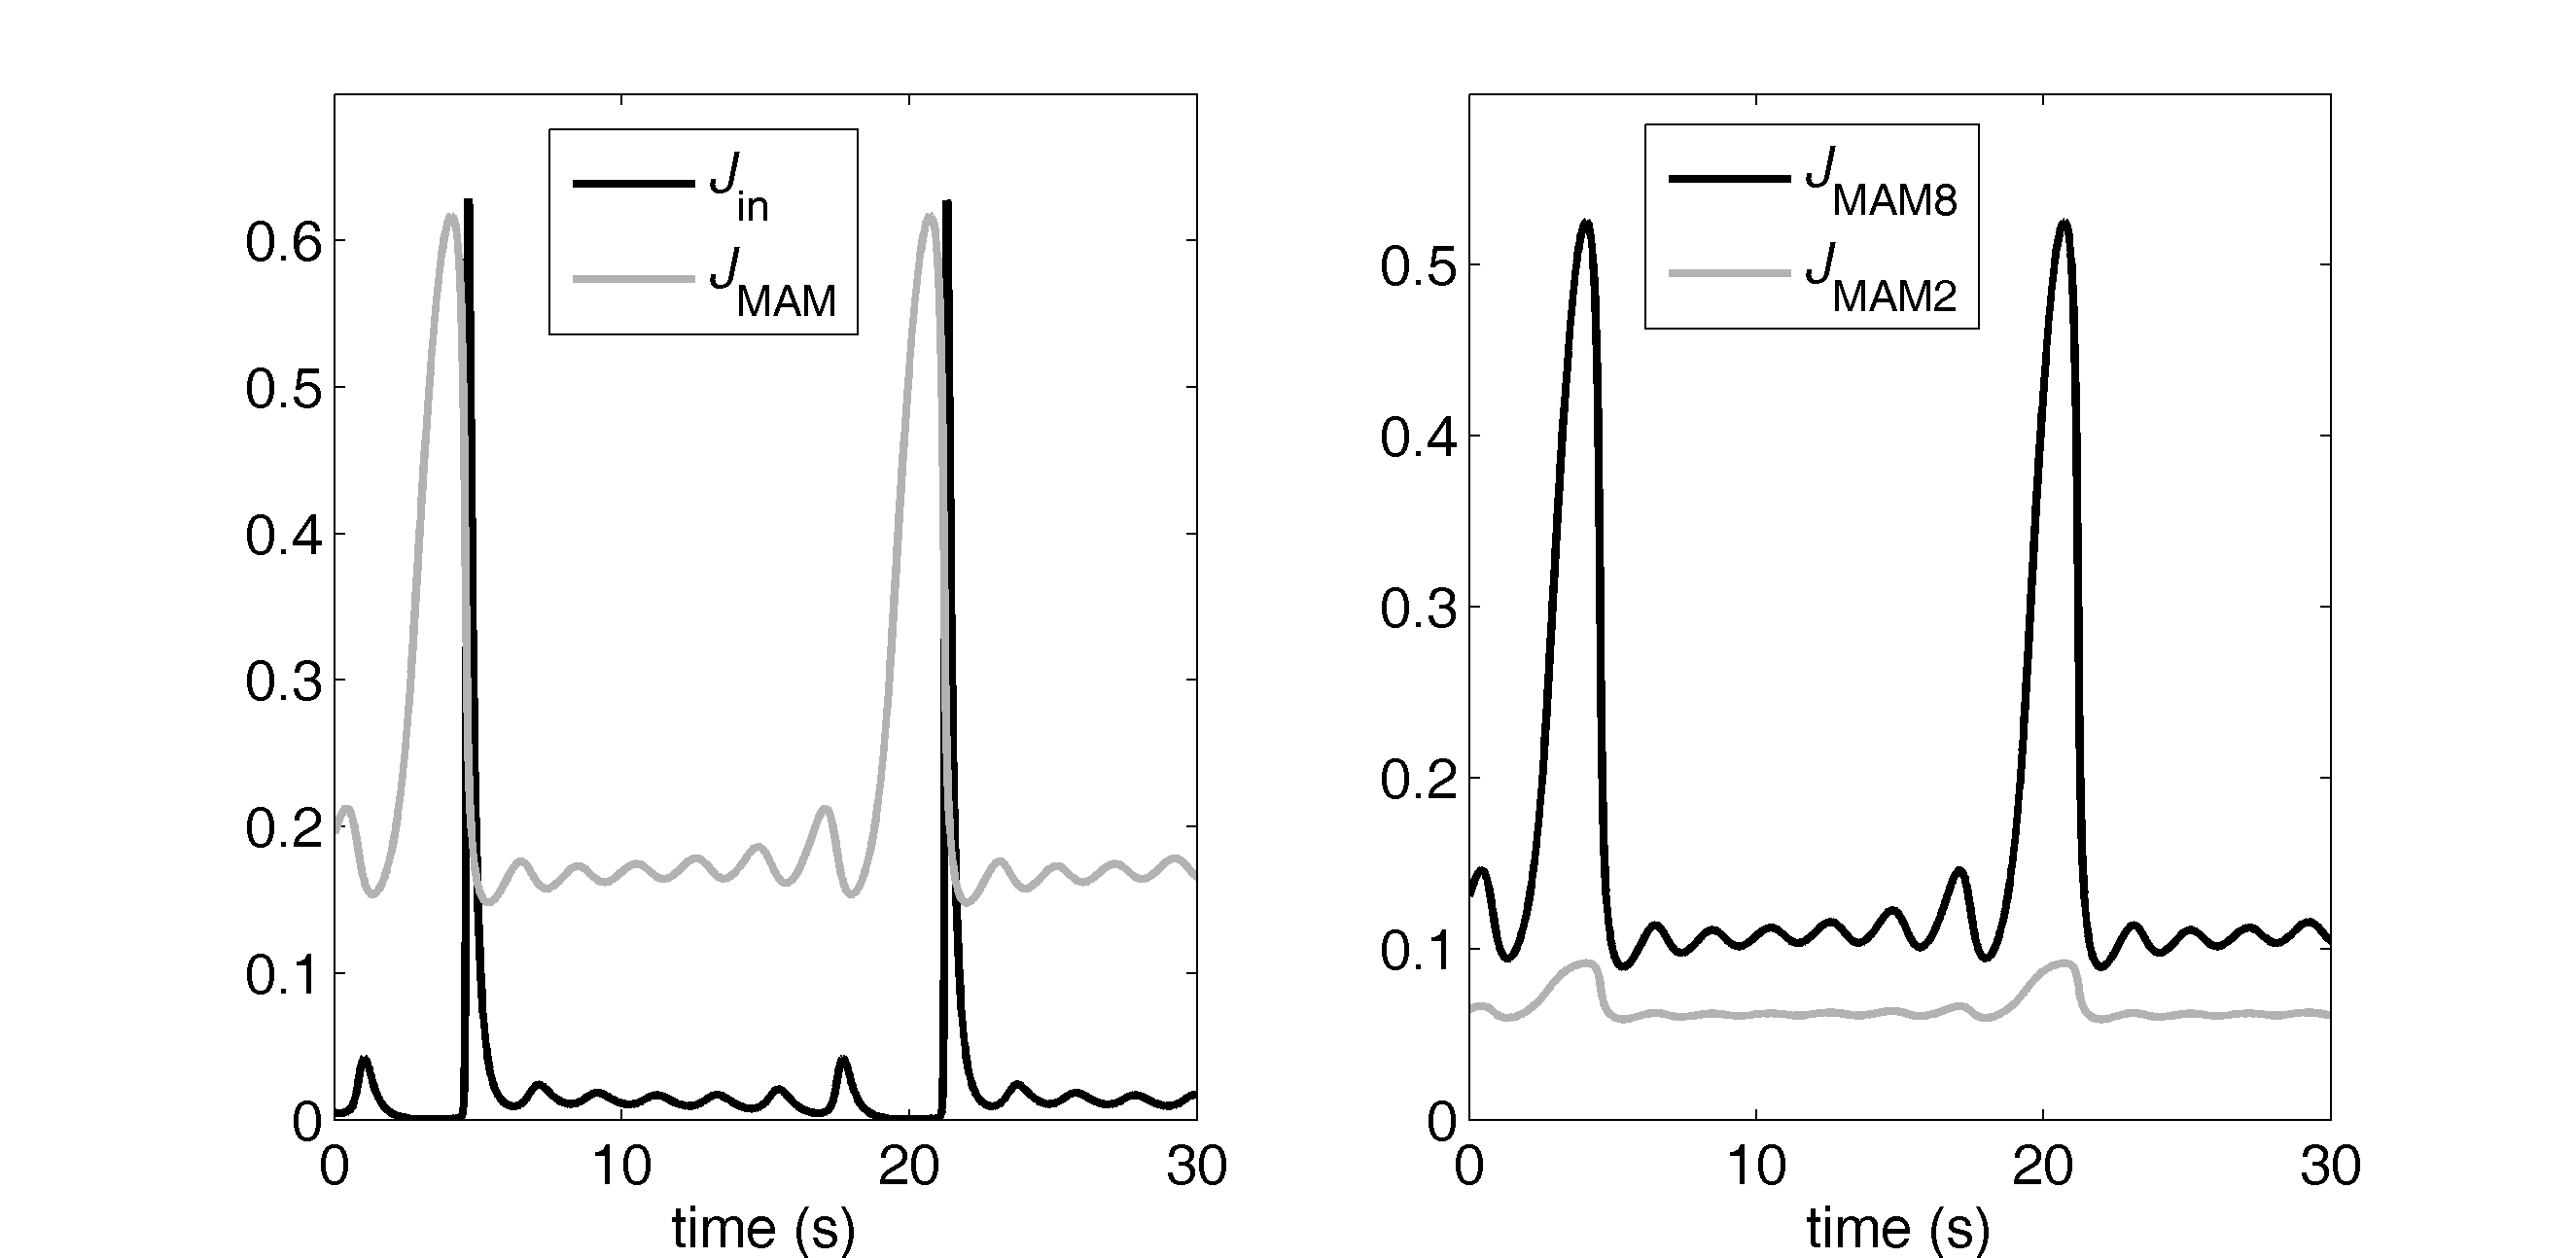
\includegraphics[width=1\textwidth]{rysunki/rozdzial_5/bursting_flowsMo2}
    \caption[Przepływy mitochondrialne w Modelu \#2]{Przebiegi czasowe mitochondrialnych przepływów wapnia dla oscylacji typu ,,bursting'' (parametry jak w Tab.~\ref{tab:constantsMo2}). Lewy panel $J_{in} = J_{in2} + J_{in8}$ i~$J_{MAM} = J_{MAM2} + J_{MAM8}$. Prawy panel $J_{MAM2}$ and $J_{MAM8}$. Wyniki  całkowania  po jednym okresie ($T \approx 16.65$s) wynoszą: $\int_{t}^{t+T} J_{in}(s) \, ds = 0.37$, $\int_{t}^{t+T} J_{MAM}(s) \, ds = 3.35$, $\int_{t}^{t+T} J_{MAM2}(s) \, ds = 1.08$ oraz $\int_{t}^{t+T} J_{MAM8}(s) \, ds = 2.47$.}
    \label{fig:przeplywy2}
\end{figure}

\FloatBarrier
\subsection{Wpływ $k_{MAM}$ na stężenia jonów wapniowych, cykle graniczne  i stany stacjonarne}


Na Ryc.~\ref{fig:minmax} widoczne są diagramy bifurkacyjne dla rozwiązań układu (\ref{eq:1aa})--(\ref{eq:5aa}) reprezentowanych przez $Ca_{Cyt}$ (lewy, górny panel), $Ca_{ER}$ (prawy, górny panel) oraz $Ca_{Mit}$ (dolny panel), z $k_{MAM}$ jako parametrem bifurkacyjnym (i innymi parametrami jak w Tab.~\ref{tab:constantsMo2}). Linia ciągła oznacza rozwiązania stabilne, natomiast linia przerywana rozwiązania niestabilne. Z diagramów tych wynika, że dla $k_{MAM} \in [0,1000]$ istnieje dokładnie jeden punkt stacjonarny $P$, który jest stabilny dla $k_{MAM}>808$, natomiast niestabilny dla $k_{MAM}\in [0, 808]$. Dla $k_{MAM}=808$ zachodzi bifurkacja typu Hopfa i dla $k_{MAM}<808$ istnieje cykl graniczny $LC_1$. $LC_1$ jest stabilny w przedziale $k_{MAM} \in [266, 808]$ i niestabilny dla $k_{MAM} \in [0,266]$. Dla wartości $k_{MAM} = 266$ następuje rozgałęzienia się cykli granicznych $LC_1$ i nowego cyklu $LC_2$. Niestabilne rozwiązanie periodyczne, łączące $LC_1$ z $LC_2$, widoczne na Ryc.~\ref{fig:minmax} jest hipotetycznym dopełnieniem do części rozwiązań znalezionych metodami numerycznymi. Cykl graniczny $LC_2$ zachowuje stabilność dla $k_{MAM} \in [0,360]$. 

\begin{figure}[ht!]
    \centering
    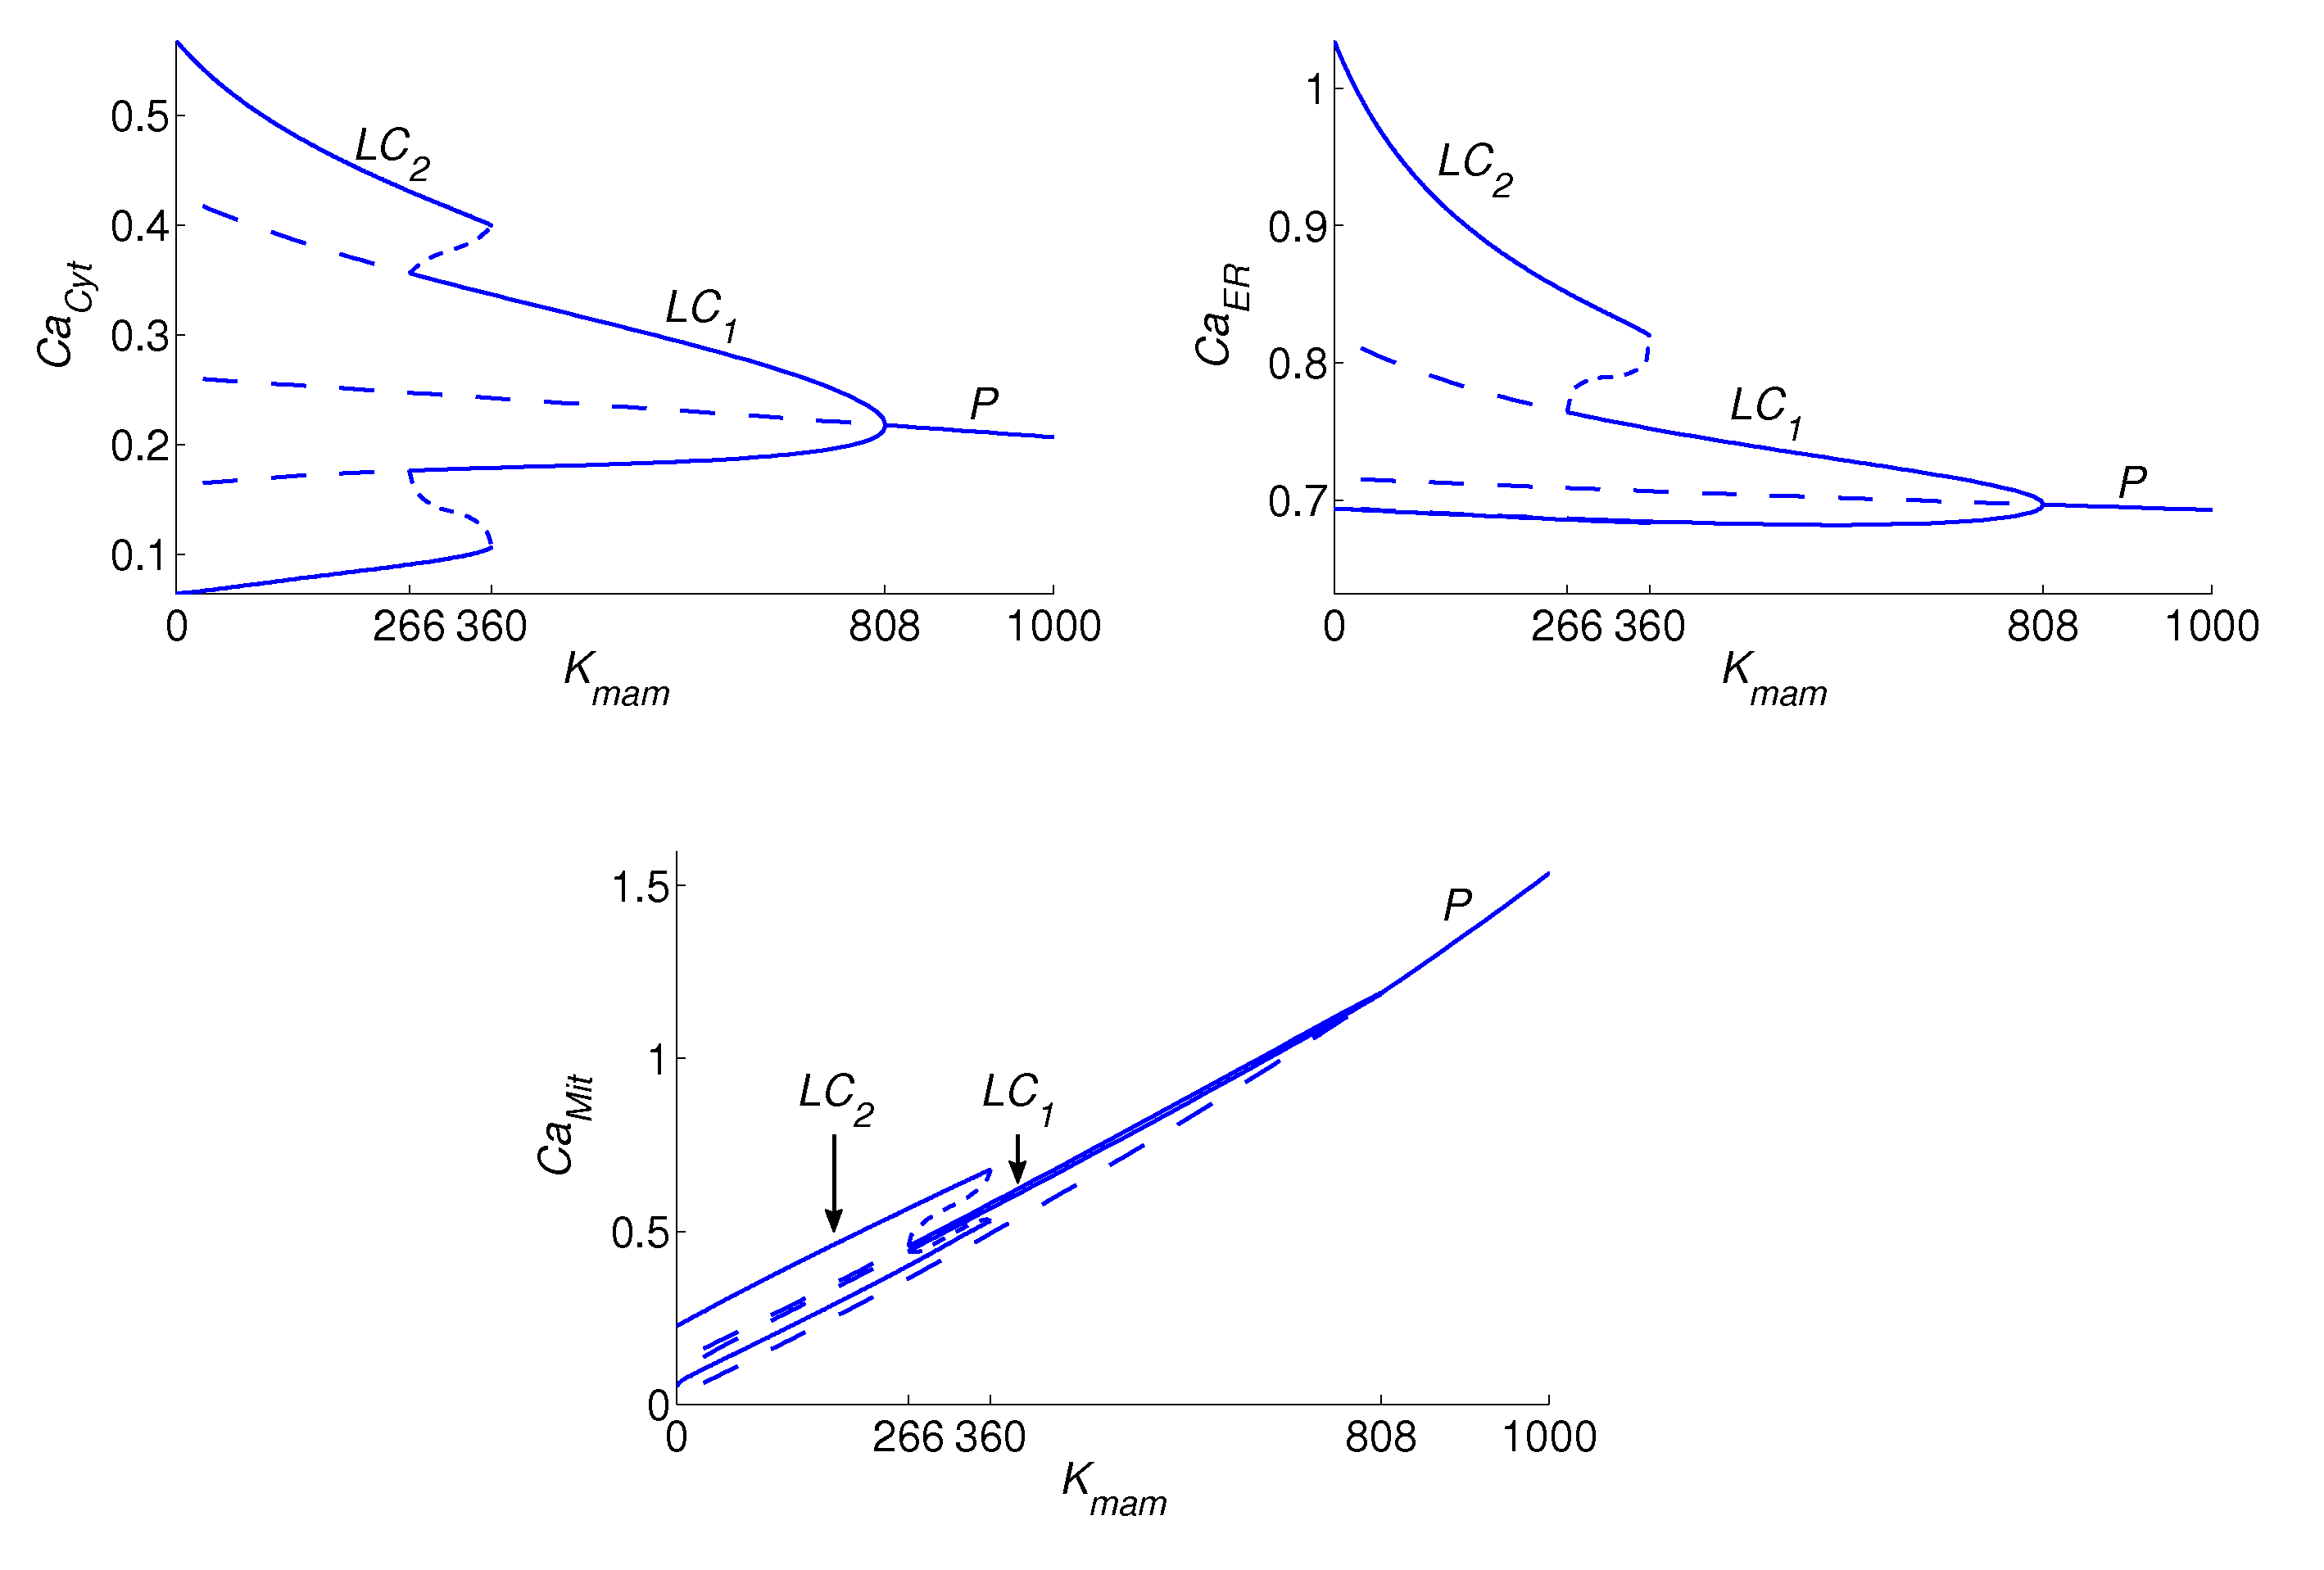
\includegraphics[width=1\textwidth]{rysunki/rozdzial_5/diagram3_1}
    \caption[Diagram bifurkacyjny dla Modelu \#2]{Diagram bifurkacyjny: $Ca_{Cyt}$ (górny, lewy panel), $Ca_{ER}$ (górny, prawy) oraz $Ca_{Mit}$ (dolny panel) z $k_{MAM} \in [0, 1000]$ jako parametrem bifurkacyjnym. Pozostałe parametry jak w Tab.~\ref{tab:constantsMo2}. Punkt stacjonarny $P$ jest stabilny dla $k_{MAM}>808$. Dla $k_{MAM}=808$ zachodzi bifurkacja typu Hopfa i pojawia się cykl graniczny $LC_1$ stabilny dla $k_{MAM} \in[266,808]$. $LC_1$ traci stabilność dla $k_{MAM}<266$. Dla $k_{MAM}<360$ istnieje stabilny cykl graniczny $LC_2$. Linia ciągła oznacza rozwiązania stabilne, natomiast linia przerywana rozwiązania niestabilne.}
    \label{fig:minmax}
\end{figure}

Z Ryc.~\ref{fig:minmax} wnioskujemy, że wzrost wartości parametru $k_{MAM}$ powoduje zmniejszenie amplitudy oscylacji oraz podwyższenie minimalnej wartości $Ca_{Mit}$. Podobne wnioski ,,bifurkacyjne'' są słuszne również dla innych wartości parametru $K_{4,8}$. Wynikają one z  analizy Ryc.~\ref{fig:freq2kmam} z rozdziału \ref{ss:MAMoscMo2}. Np. dla $K_{4,8} = 1.5$ zmianie ulegają wartości parametru $k_{MAM}$, dla których dochodzi do bifurkacji typu Hopfa ($k_{MAM} = 238$) oraz rozgałęzienia cykli granicznych ($k_{MAM} = 80$).

\begin{figure}[ht]
    \centering
    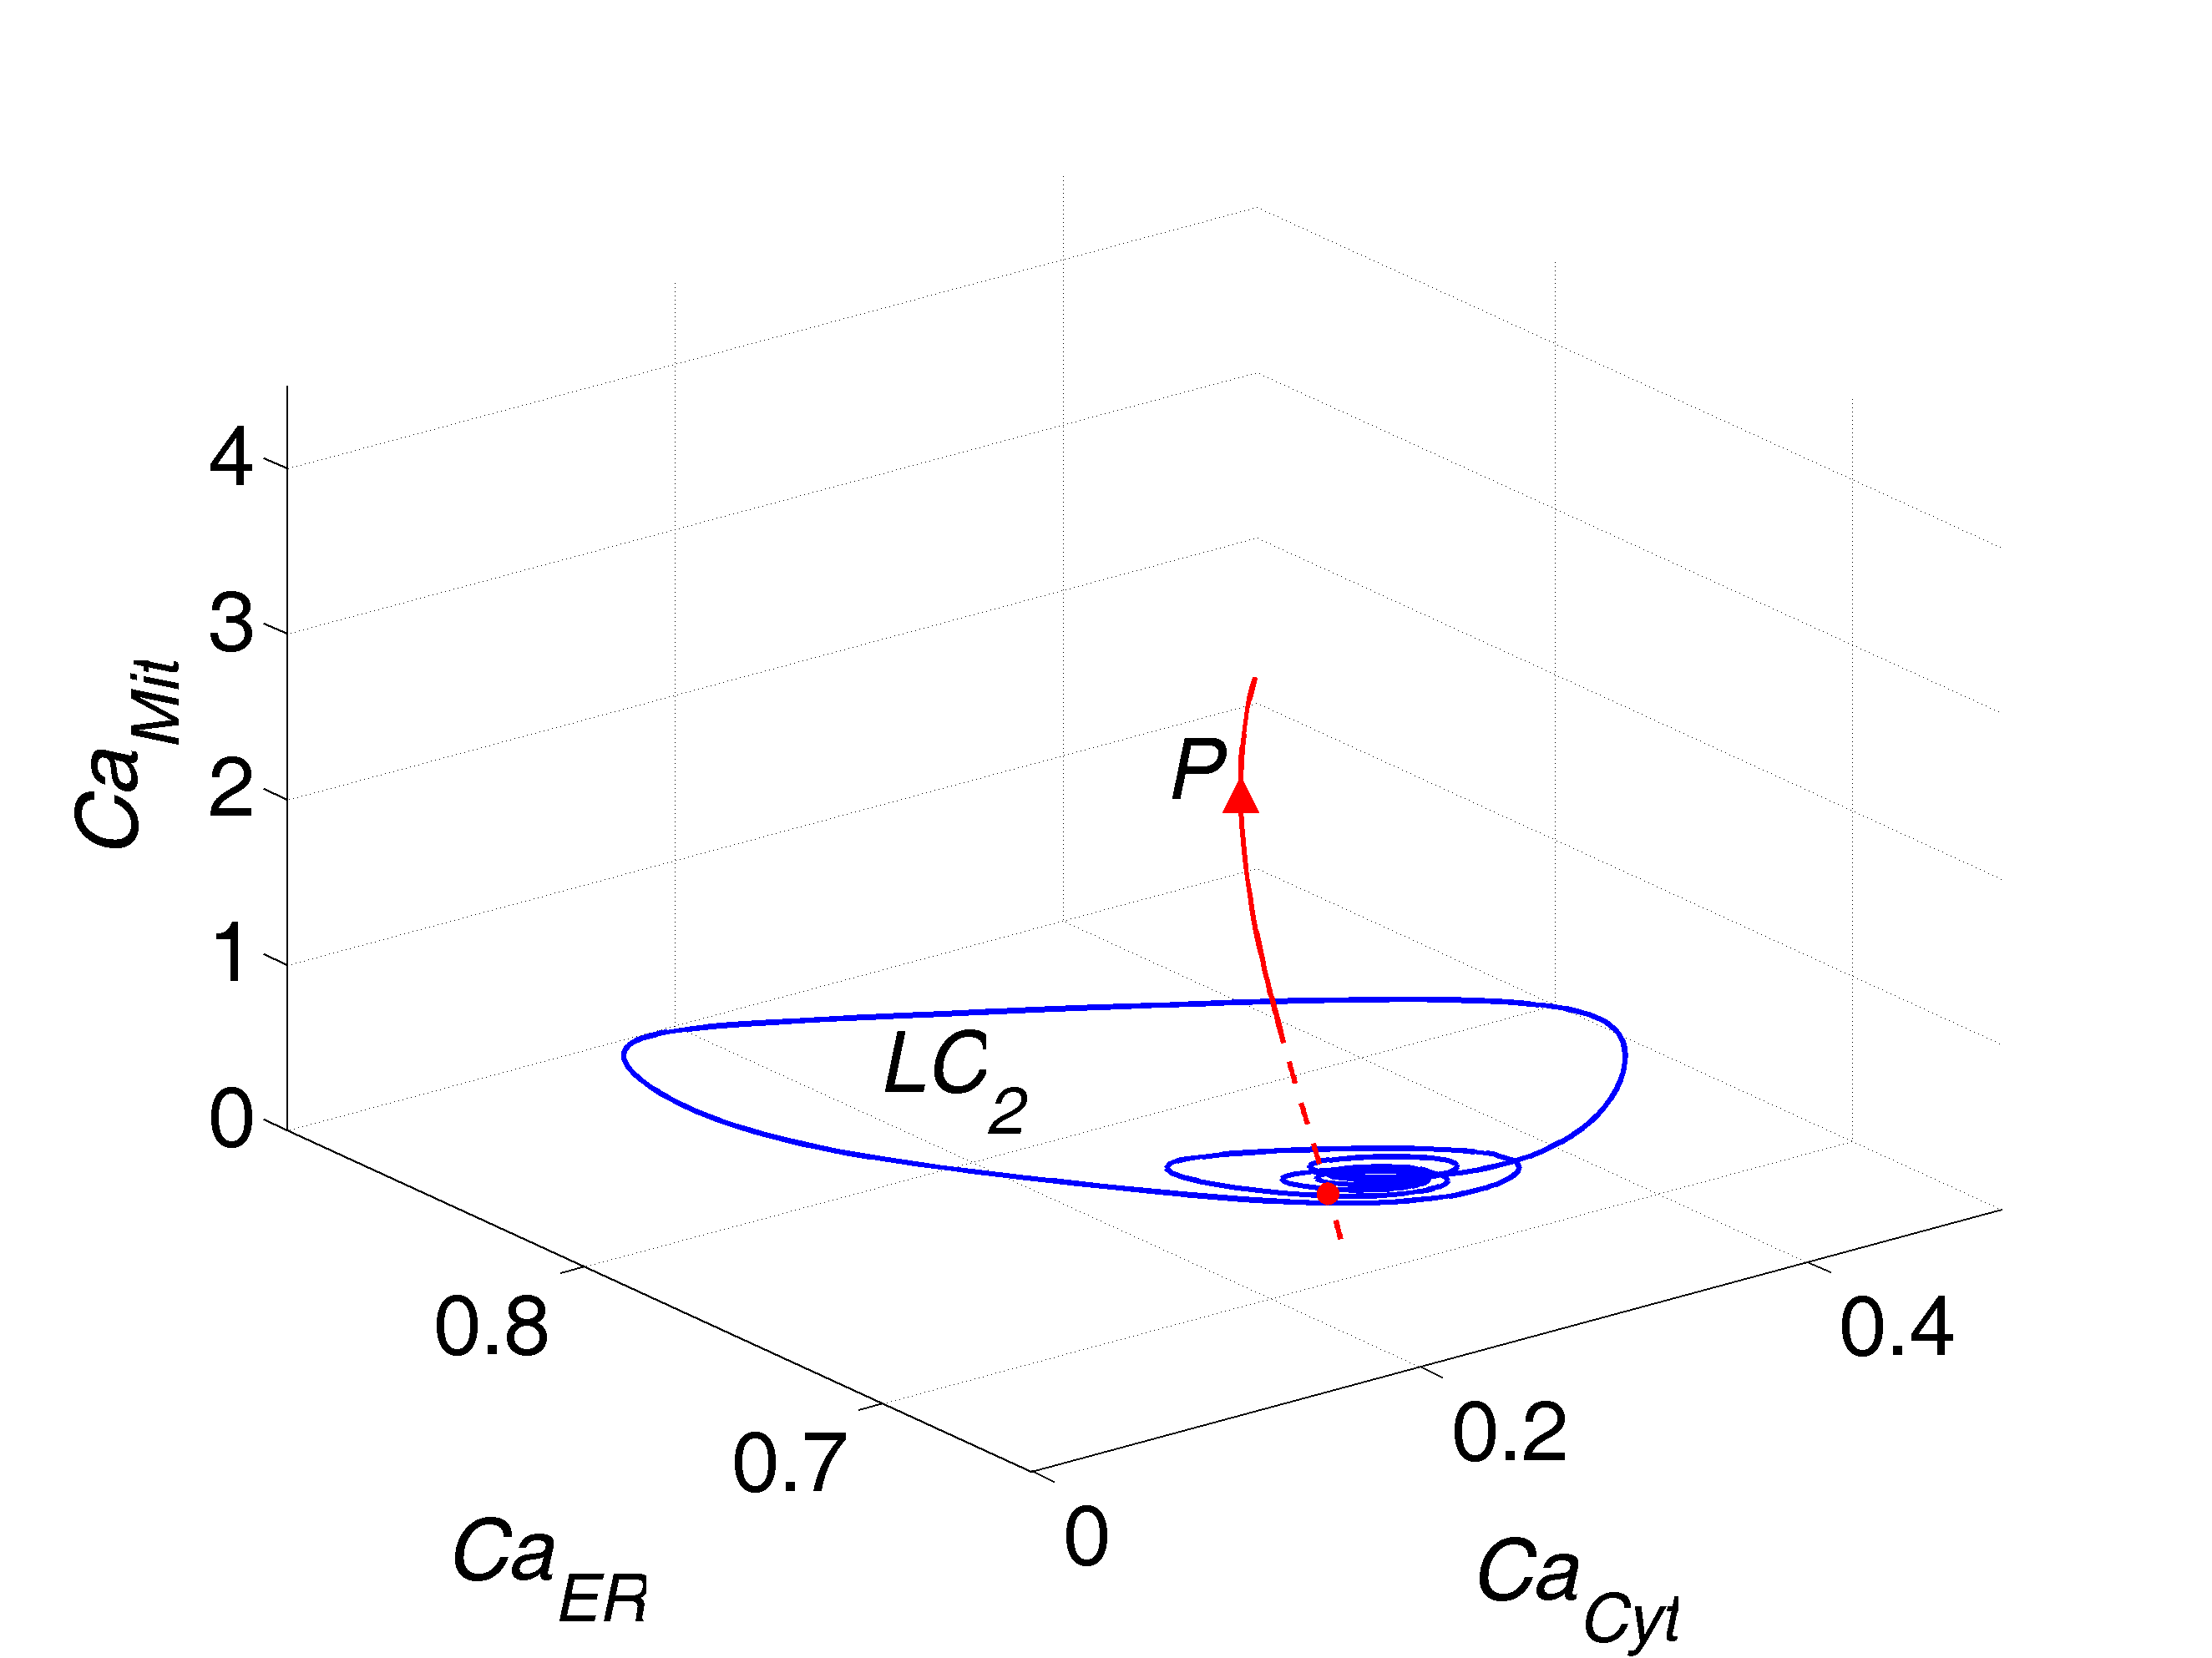
\includegraphics[width=1\textwidth]{rysunki/rozdzial_5/diagram3_5}
    \caption[Portret fazowy 3-D oscylacji typu ,,bursting''w Modelu \#2]{Portret fazowy 3-D oscylacji typu ,,bursting'' dla $K_3=3.5$ i pozostałych parametrach jak w Tab.~\ref{tab:constantsMo2} i ,,ścieżka'' stanu stacjonarnego dla $k_{MAM} \in [0, 2000]$. Kierunek wzrostu wartości parametru $k_{MAM}$ oznaczono strzałką. Linia przerywana oznacza niestabilne stany stacjonarne, linia pełna - stabilne. Bifurkacja Hopfa zachodzi dla $k_{MAM} = 864$ i jest oznaczona jako pogrubiony punkt.}
    \label{fig:diagram3_5}
\end{figure}


Na Ryc. \ref{fig:diagram3_5} widoczny jest stabilny cykl graniczny $LC_2$ dla $k_{MAM} = 250$, $K_3 = 3.5$ oraz pozostałych parametrów jak w Tab.~\ref{tab:constantsMo2} (niebieska krzywa). Krzywa czerwona przedstawia ścieżkę punktu stacjonarnego $P$ dla $K_3 = 3.5$ i $k_{MAM}$ z przedziału [0,2000]. Linia ciągła krzywej czerwonej odpowiada stabilnym stanom stacjonarnym ($k_{MAM} > 864$), natomiast linia przerywana odpowiada stanom niestabilnym. Strzałka wskazuje kierunek wzrostu wartości parametru $k_{MAM}$. Czerwony punkt widoczny na wykresie przedstawia punkt stacjonarny dla wartości  $k_{MAM}=k_{MAM2}+k_{MAM8}=50+200=250$ (tak jak w referencyjnym zestawie parametrów podanym w Tab.~\ref{tab:constantsMo2}). 
Dla $k_{MAM} > 864$ stabilny punkt stacjonarny $P$ jest jedynym atraktorem układu, tak więc wszystkie trajektorie zbiegają do niego asymptotycznie w czasie. Punkt ten charakteryzuje się wysoką, rosnącą wraz z $k_{MAM}$ wartością $Ca_{Mit}$. Np. dla $k_{MAM} = 1000$ $Ca_{Mit} = 1.84$, natomiast dla  $k_{MAM} = 2000$ $Ca_{Mit} = 4.24$. Zatem odpowiednio duży przepływ przez struktury MAM (odpowiadający dużym wartościom parametru $k_{MAM}$) wymusza przejście systemu do stanu, w którym wapń akumulowany jest w kompartmencie mitochondrialnym, co stanowi początkowy etap procesu apoptozy. Zagadnienie to zostanie opisane w Rozdz.~\ref{s:scenariusz}.


\FloatBarrier
\subsection{Wpływ współczynnika $k_{MAM}$ na okres oscylacji}
\label{ss:MAMoscMo2}

W niniejszym rozdziale badamy wpływ parametrów  $K_{4,8}$ i $k_{MAM}$ na okres oscylacji. Ze względu na fakt, iż niestabilne rozwiązania periodyczne nie mają znaczenia z biologicznego punktu widzenia, analizę ograniczamy do stabilnych ,,odcinków'' cykli granicznych $LC_1$ i~$LC_2$. Wybrane wartości parametrów to: $K_{4,8}= 1.5, 1.8 \textrm{ i } 2.1$ oraz $0 \leq k_{MAM} \leq 260$. Ze względu na inne wartości parametru $K_{4,8}$  w stosunku do przypadku analizowanego na Ryc~\ref{fig:minmax} obszary $k_{MAM}$, dla których cykle graniczne $LC_1$ i~$LC_2$ są stabilne różnią się od obszarów widocznych na tej rycinie.


\begin{figure}[ht]
    \centering
    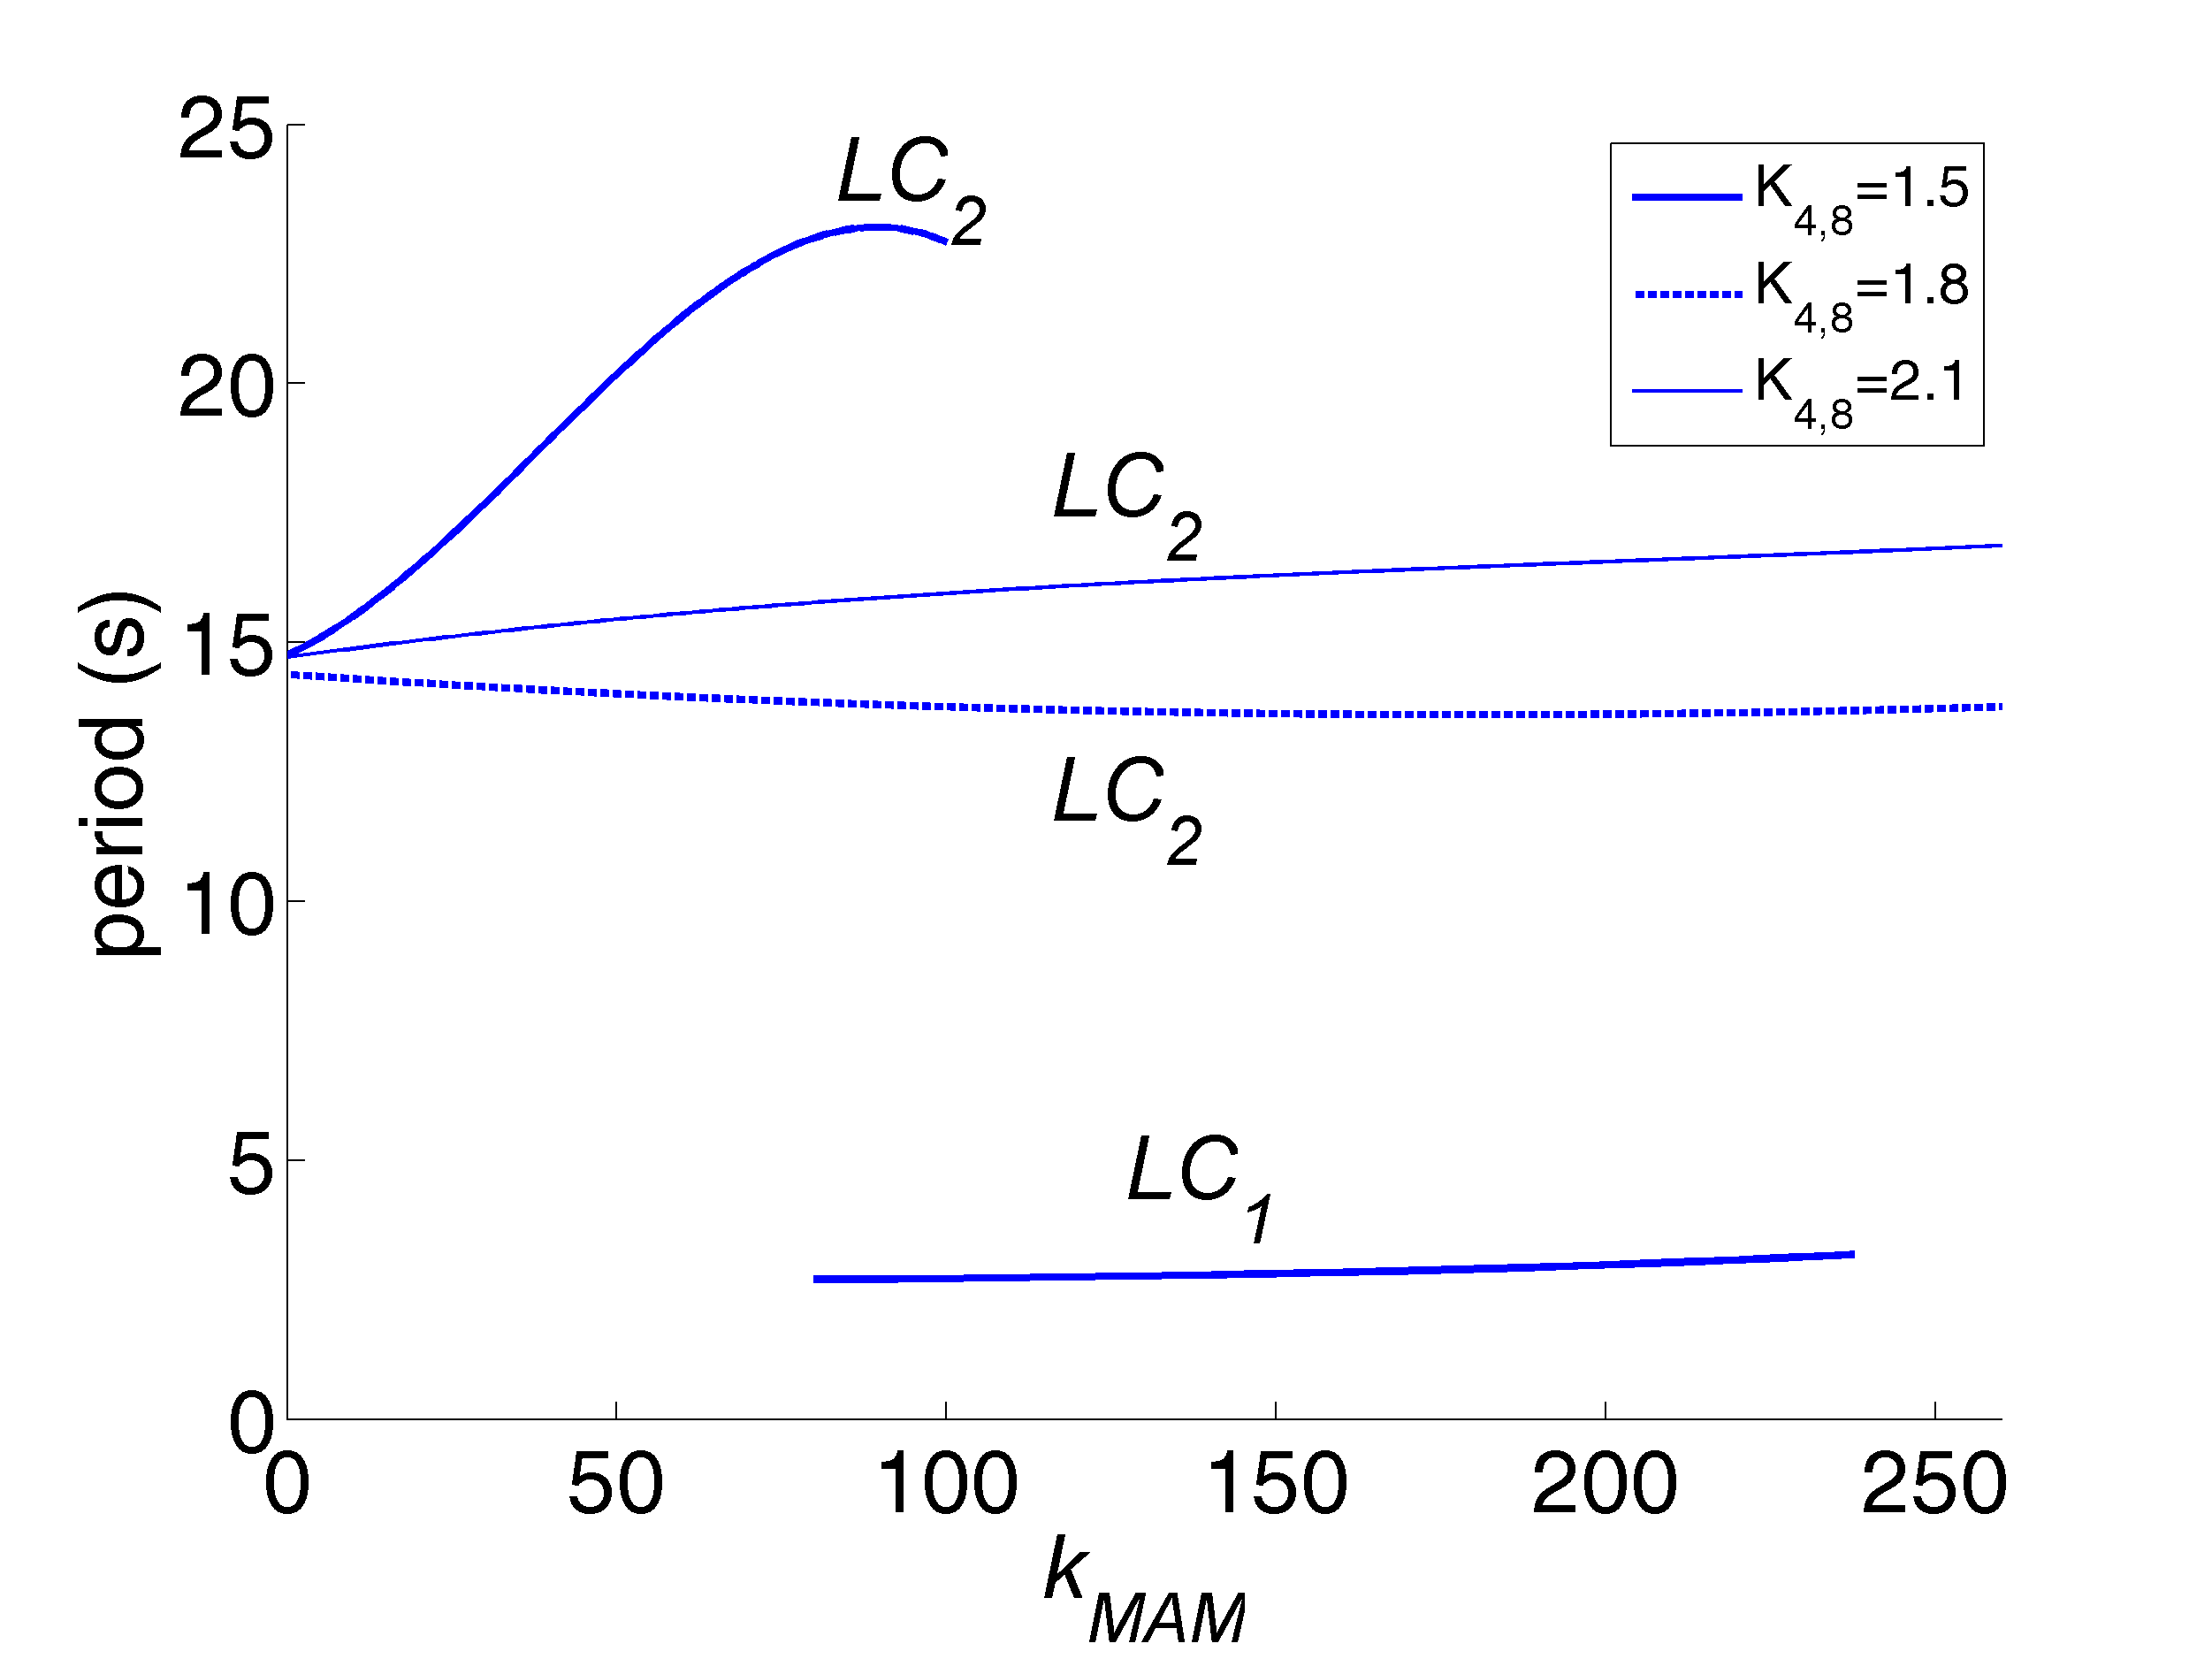
\includegraphics[width=1\textwidth]{rysunki/rozdzial_5/periodlc.png}
    \caption[Stabilne oscylacje jako funkcja parametrów $k_{MAM}$ i $K_{4,8}$]{Wykres stabilnych oscylacji jako funkcja parametrów $k_{MAM}$ i $K_{4,8}$. Pozostałe parametry jak w Tab.~\ref{tab:constantsMo2}.}
    \label{fig:freq2kmam}
\end{figure}


Wyniki analizy przedstawiono na Ryc.~\ref{fig:freq2kmam}. Dla $K_{4,8}=2.1$ okres jest niemal stały i~zmienia się z 14.7 (dla $k_{MAM}=0$) do 16.9 (dla $k_{MAM}=260$). Podobnie dla $K_{4,8}=1.8$ okres jest prawie stały i maleje z 14.4 (dla $k_{MAM}=0$) do 13.8 (dla $k_{MAM}=260$). Dla tych wartości parametru $K_{4,8}$ cykl graniczny $LC_1$ jest niestabilny dla  $k_{MAM} < 260$, dlatego też nie uwzględniliśmy okresów dla tego cyklu granicznego w~podanym wcześniej przedziale $k_{MAM}$ na rycinie.

Dla $K_{4,8}=1.5$ zachowanie modelu zmienia się drastycznie. Okres oscylacji $LC_2$ wzrasta silnie od 14.8 s (dla $k_{MAM}=0$) do 22.7 s (dla $k_{MAM}=100$). Przy wartości $k_{MAM} \approx 100$ okres stabilnych oscylacji maleje do 2.7. Spowodowane jest to tym, iż dla tej wartości $k_{MAM}$ cykl graniczny $LC_2$ traci stabilność. Cykl graniczny $LC_1$ istnieje dla $k_{MAM} \leq 238$ i zachowuje stabilność dla $k_{MAM} \geq 80$.


\subsection{Podsumowanie dotyczące Modelu \#2}
Zaproponowaliśmy nowy model wewnątrzkomórkowych oscylacji stężeń jonów wapnia, który bierze pod uwagę istnienie kompleksów błonowych pomiędzy mitochondriami oraz ER (tzw. MAM). Stanowią one miejsca kontaktu obu organelli. Model ten stanowi modyfikację wcześniejszego  modelu \cite{Marhl2000}. Modyfikacje polegały na wprowadzeniu bezpośredniego przepływu jonów wapnia z retikulum endoplazmatycznego do mitochondriów w postaci przepływu $J_{MAM}$. W stosunku do Modelu \#1 rozpatrzyliśmy dokładniejsze postaci przepływów $J_{MAM}$ i $J_{in}$ (\ref{eq:jmamMo2}), (\ref{eq:jinMo2}). W obu przepływach uwzględniliśmy zatem dwie składowe wpływu wapnia do mitochondrium, które odpowiadają modułom pracy uniportera: trybowi normalnemu oraz trybowi RaM. Zmodyfikowany został również przepływ $J_out$, który w pracy \cite{Marhl2000} oraz w Modelu \#1, zależy od cytozolicznego stężenia jonów wapnia $Ca_{Cyt}$ (\ref{eq:joutMo1}). W Modelu \#2 funkcja opisująca przepływ $J_{out}$ bazuje na \cite{Magnus1997,Mazel2009} i zamieszczonych tam referencjach. W Modelu \#2 wypływ jonów wapnia z mitochondriów opisany równaniem (\ref{eq:joutMo2}) zależy wyłącznie od stężenia tych jonów w przedziale mitochondrialnym ($Ca_{Mit}$). To zasadnicza różnica pomiędzy Modelem \#2, a Modelem \#1, która powoduje, że układ nie jest w stanie generować rozwiązań chaotycznych.

Zbadaliśmy numerycznie wpływ struktur MAM  na okres i profil przebiegów czasowych rozwiązań periodycznych. Symulacje numeryczne wykazały istnienie wyłącznie oscylacji typu ,,bursting''. Zbadaliśmy również  wpływ parametru $k_{MAM}$ na rozwiązania periodyczne i punkty stacjonarne. Wykazaliśmy, że dla pewnych wartości parametru $K_{4,8}$ istnieją przedziały $k_{MAM}$, dla których współistnieją dwa cykle graniczne $LC_1$ i $LC_2$, różniące się amplitudą  i okresem oscylacji. Cykl graniczny $LC_1$ o mniejszym okresie i mniejszej amplitudzie oscylacji staje się stabilny  dla odpowiednio wysokich wartości parametru $k_{MAM}$. Ostatecznie dla odpowiednio wysokich wartości $k_{MAM}$ rozwiązania periodyczne zanikają, a większość trajektorii przyciągana jest przez stabilny punkt stacjonarny $P$, charakteryzujący się wysokim poziomem jonów wapnia w mitochondriach (Ryc.~\ref{fig:diagram3_5}). Wejście układu na jedną z takich trajektorii może być interpretowane jako początek procesu apoptozy.

\FloatBarrier
\section{Scenariusz apoptozy}\label{s:scenariusz}

Mitochondria pełnia kluczową rolę w procesie apoptozy, są też kluczowymi organellami utrzymującymi homeostazę wapniową w komórce. Zgodnie z przyjętym modelem szlaku wewnętrznego apoptozy, jednym z najważniejszych i koniecznych zdarzeń W~trakcie realizacji programowanej śmierci jest uwolnienie cytochromu C z przestrzeni perymitochondrialnej. W tym celu musi dojść do fragmentacji zewnętrznej błony mitochondrialnej \cite{VanderHeiden1997}. Zgodnie z tą teorią jony (w tym jony wapnia), przedostające się do matriks mitochondriów, zwiększają ciśnienie osmotyczne w matrix, powodując przepływ cząsteczek wody w kierunku bardziej stężonego roztworu, powodując wzrost objętości organelli, potocznie nazywany ,,pęcznieniem mitochondriów''. Ponieważ wewnętrzna błona mitochondrialna posiada szereg wpukleń (tzw. grzebieni mitochondrialnych), jej powierzchnia jest kilkakrotnie większa od powierzchni błony zewnętrznej (por.~\ref{app:b}). Rozszerzanie się wewnętrznej błony w wyniku zwiększenia objętości matriks może prowadzić do utraty ciągłości zewnętrznej błony mitochondrialnej.

W niniejszej pracy wykazaliśmy, że dla specyficznego zestawu parametrów oba modele pozwalają na wygenerowanie takiego stanu badanego systemu, który charakteryzuje się wysokim stężeniem jonów wapnia w kompartmencie mitochondrialnym. 

W \textbf{Modelu \#1} dla $k_{ch}=2950$ i $k_{MAM} \leq 101$ oraz  $k_{ch} = 4100$ i $k_{MAM} < 1649$ istnieje stabilny cykl graniczny lub chaotyczne trajektorie, charakteryzujące się dużym basenem przyciągania. Zachowania układu zmieniają się jednak wraz ze wzrostem wartości $k_{MAM}$, która charakteryzuje wielkość przepływu jonów Ca$^{2+}$ przez interfejs MAM. Dla współczynników  $k_{ch}=2950$ i $k_{MAM} \geq 102$ oraz $k_{ch} = 4100$ i $k_{MAM} \geq 1649$ większość trajektorii zbiega do punktu stacjonarnego, który charakteryzuje się bardzo wysokim stężeniem jonów wapnia w mitochondrium ($Ca_{Mit}>18 \mu$M -- punkt $P_1$ na Ryc.~\ref{fig:steadystatesMo1}).

W \textbf{Modelu \#2}  (dla $k_{MAM} > 864$) oraz  $K_3 = 3.5$ istnieje stabilne rozwiązanie - punkt $P$, które charakteryzuje się wysokim stężeniem jonów wapniowych w przedziale mitochondrialnym (Ryc.~\ref{fig:diagram3_5}). Dla $k_{MAM} > 864$ punkt $P$ jest jedynym atraktorem systemu, tak więc wszystkie trajektorie zbiegają do tego stabilnego stanu stacjonarnego. Punkt ten charakteryzuje się wysoką i rosnącą wartością $Ca_{Mit}$, która rośnie wraz ze wzrostem wartości parametru $k_{MAM}$. Np. dla $k_{MAM} = 1000$ $Ca_{Mit} = 1.84$, natomiast dla  $k_{MAM} = 2000$ $Ca_{Mit} = 4.24$. 

W każdym z opisanych modeli wykazaliśmy, że zwiększanie przepływu jonów wapnia przez struktury MAM poprzez manipulację parametrem $k_{MAM}$ doprowadza do zaniku stabilnych rozwiązań oscylacyjnych, w wyniku czego w systemie występuje tylko jedno rozwiązanie stabilne - punkt stacjonarny o wysokim stężeniu jonów wapniowych w~kompartmencie mitochondrialnym.

Jak wiadomo, podwyższenie poziomu wapnia w mitochondriach towarzyszy początkowym etapom procesu apoptozy \ref{s:apoptoza}. Gromadzenie się jonów Ca$^{2+}$ może wynikać ze zwiększonego przepływu jonów wapniowych do mitochondrium z ER poprzez struktury MAM. Dane eksperymentalne wskazują, że wiele czynników stresogennych wpływa na ekspresję białek związanych z powstawaniem połączeń pomiędzy mitochondriami i ER. Park i współpracownicy wykazali, że stres cieplny powoduje wzrost ilości transkryptów kalretikuliny (bufora wapniowego)  \cite{Park2001}. Także szereg innych białek retikularnych, współtworzących struktury MAM, takich jak erp44, hsp90, grp94, grp75 czy receptor \mbox{sigma-1} podlegać może nadekspresji, w wyniku działania różnych czynników stresogennych (m.in. stres oksydacyjny, niedoboru związków odżywczych, stres cieplny lub wywołany specyficznym ligandem) \cite{Anelli2002,Ellgaard2001,Hayashi2007}. Nie tylko czynniki związane ze stresem mają wpływ na ilość struktur MAM. Ilość miejsc kontaktu regulować mogą także białka modulujące kształt mitochondriów np. mitofuzyna-1 lub mitofuzyna-2. Doświadczenia ze zmutowanymi liniami komórkowymi, które charakteryzowały się brakiem mitofuzyny-2 (MFN-2 $^{-/-}$), wykazały że komórki MFN-2 $^{-/-}$ posiadały aż 40\% mniej połączeń pomiędzy ER i mitochondriami, co miało duży wpływ na transport wapnia do mitochondriów. Z kolei nadekspresja mitofuzyny-2 i zwiększenie połączeń ER-Mit jest wystarczające do wywołania apoptozy w komórkach mięśni gładkich naczyń krwionośnych \cite{Guo2007}. Dodatkowo ekspozycja na intensywny stres cieplny wywołuje wzmożoną glikozylację białek chaperonowych (w~tym kalretikuliny) \cite{Jethmalani1998}. Glikozylacja powoduje powstawanie bardziej stabilnych kompleksów białkowych, wliczając w to białka budujące MAM \cite{Mizzen1991}. Ponieważ chaperony ER są niezbędne do prawidłowego przepływu jonów wapnia z ER do mitochondrium, stabilizacja połączeń powoduje, że mitochondria są w stanie przyjąć znaczne ilości jonów wapnia. Krótkotrwały stres i~przepływ wapnia do mitochondriów może mieć działanie anty-apoptotyczne. W przypadku, kiedy podwyższony poziom jonów wapnia w mitochondriach utrzymuje się przez relatywnie długi czas, może to skutkować ,,pęcznieniem mitochondriów'', co z kolei może prowadzić do wejścia komórki na szlak apoptotyczny (uwolnienie cytochromu C, AIF, aktywacja kaspazy-9) \cite{Giorgi2012a,Hajnoczky2006,Rasola2007}.